%%%%%%%%%%%%%%%%%%%%%%%%%%%%%%%%%%%%%%%%%%%%%%%%%%%%%%%%%%
%%%%%%%%%%%%         PREAMBLE         %%%%%%%%%%%%

%% Default settings format a final copy (12pt font, single-sided,
%% double-spaced, normal margins, single-spaced notes).  For a rough
%% copy (10pt font, double-sided, double-spaced, normal margins, with
%% the word "DRAFT" printed at each corner of every page), use the
%% `draft' option.  The default line spacing can be changed with one
%% of the following options: `singlespaced', `oneandahalfspaced', or
%% `doublespaced'.  The notes are always single-spaced by default, but
%% can be made to have the same spacing as the rest of the document by
%% using the option `spacednotes'.  The size of the margins can be
%% changed with one of the following options: `narrowmargins' (1 1/4"
%% left, 3/4" others), `normalmargins' (1 1/4" left, 1" others),
%% `widemargins' (1 1/4" all), `extrawidemargins' (1 1/2" all).  Any
%% other standard option for the `report' document class can be used
%% to override the default or draft settings.

%% ***   Add any desired options.   ***
\documentclass[letterpaper]{ut-thesis} % For Single Sided
%\documentclass[letterpaper,twoside,10pt]{ut-thesis} % For Double Sided
%% ***   Add \usepackage declarations here.   ***
% Setting up graphics
\usepackage{ifpdf}

\ifpdf
\usepackage[pdftex]{graphicx}
\usepackage[protrusion=true,expansion=true]{microtype}
\else
\usepackage{graphicx}
\fi

\usepackage{longtable}
\usepackage{amsmath,amssymb,multirow,dcolumn,fancyhdr,charter,graphicx,color}
\usepackage{xspace}
\usepackage[hyphens]{url}

% Symbol Stuff
\usepackage{latexsym}%
\usepackage{amssymb}%

% Bibliography Stuff 
\usepackage{natbib}
\setcitestyle{aysep={},yysep={;}}

% AAS Tex Stuff
\usepackage{aastex_hack}
\usepackage{deluxetable}
\usepackage[labelsep=colon,small]{caption}

% Fonts
% Using Better Fonts
\usepackage[sc]{mathpazo}
\usepackage[T1]{fontenc}

% Paragraph Spacing Issue:
\setlength{\parskip}{0cm plus1mm minus1mm}

%commenting
\def\memohr#1{\color{blue}$HR[${\bf #1}$]$ \color{black}}
\def\memoas#1{\color{red}$AS[${\bf #1}$]$ \color{black}}

%% The line spacing of the document should be specified using one of
%% the document options given above, but if you need a line spacing
%% that is not provided by the options, you can override the default
%% line spacing for the entire document with the command
%%   `\linespacing{...}'.
%% Note that in order to get the correct appearance, the argument to
%% `\linespacing' must be equal to 1/3 + 2/3 times the desired line
%% spacing (for example, single-spaced = \linespacing{1},
%%                        1 1/2-spaced = \linespacing{1.33}, and
%%                       double-spaced = \linespacing{1.66}).

%% ***   Uncomment and fill in a value, if needed.    ***
%% ***   REMEMBER: You should NOT need to use this.  Use one of   ***
%% ***   the document class options mentionned above instead.     ***
%\linespacing{}

%%%%%%%%%%%%%%%%%%%%%%%%%%%%%%%%%%%%%%%%%%%%%%%%%%%%%%%%%%%%%%%%%%%%%%
%%                                                                  %%
%%                  ***   I M P O R T A N T   ***                   %%
%%                                                                  %%
%%  Fill in the following fields with the required information:     %%
%%   - \degree{...}       name of the degree obtained               %%
%%   - \department{...}   name of the graduate department           %%
%%   - \gradyear{...}     year of graduation                        %%
%%   - \author{...}       name of the author                        %%
%%   - \title{...}        title of the thesis                       %%
%%%%%%%%%%%%%%%%%%%%%%%%%%%%%%%%%%%%%%%%%%%%%%%%%%%%%%%%%%%%%%%%%%%%%%

%% ***   Change this example to appropriate values.   ***
\degree{Doctor of Philosophy} \department{Astronomy \& Astrophysics}
\gradyear{2017} \author{Ari Silburt} \title{Statistics, Formation and Stability of Exoplanetary Systems}

%% ***   NOTE   ***
%% Put here all other formatting commands that belong in the preamble.


%% For example, to list only down to subsections in table of contents
%% (-1=part, 0=chapter, 1=section, 2=subsection, 3=subsubsection,
%%  4=paragraph, 5=subparagraph, 6=subsubparagraph).
%
\setcounter{tocdepth}{2}


%%%%%%%%%%%%      MAIN  DOCUMENT      %%%%%%%%%%%%

\begin{document}


%% ***   NOTE   ***
%% You should put all of your `\newcommand', `\newenvironment', and
%% `\newtheorem's (in other words, all the global definitions that
%% you will need throughout your thesis) in a separate file and use
%% "\input{filename}" to input it here.

%%% Add your own personal commands in here


\newcommand       \micronm      {\,\mu{\rm m} }
\newcommand       \HII          {\ion{H}{2}}
\newcommand       \kpc		{\,{\rm kpc }}
\newcommand       \kms		{\,{\rm km\,s^{-1} }}
\newcommand       \erg		{\,{\rm erg }}
\newcommand       \s		{\,{\rm s }}
\newcommand       \pc		{\,{\rm pc }}
\newcommand       \hii          {\ion{H}{2} }
\newcommand       \eightum      {$\,8\,\mu{\rm m}$ }
\newcommand       \jmag         {\,$J$}
\newcommand       \hmag         {\,$H$} 
\newcommand       \kmag         {\,$K_{S}$} 
\newcommand       \jh           {\,$J-H$} 
\newcommand       \hk           {\,$H-K_{S}$}

%% This sets the page style and numbering for preliminary sections.
\begin{preliminary}

%% This generates the title page from the information given above.
\maketitle

%% There should be NOTHING between the title page and abstract.

%% This generates the abstract page, with the line spacing adjusted
%% according to SGS guidelines.
\begin{abstract}
  
Over the past two decades scientists have detected thousands of exoplanets through a variety of methods, and collective properties of exoplanetary systems are now emerging. 
This thesis contributes to the exoplanet field by analyzing the statistics, formation and stability of exoplanetary systems.

The first part of this thesis conducts a statistical reconstruction of the radius and period distributions of \kep planets. 
Accounting for observation and detection biases, as well as measurement errors, we calculate the occurrence of planetary systems, including the prevalence of Earth-like planets.
This calculation is compared to related works, finding both similarities and differences. 
 
Second, the formation of \kep planets near mean motion resonance (MMR) is investigated.
In particular, 27 \kep systems near 2:1 MMR are analyzed to determine whether tides are a viable mechanism for transporting \kep planets from MMR.
We find that tides alone cannot transport near-resonant planets from exact 2:1 MMR to their observed locations, and other mechanisms must be invoked to explain their formation.

Third, a new hybrid integrator \hermes is presented, which is capable of simulating N-bodies undergoing close encounters.
\hermes is specifically designed for planets embedded in planetesimal disks, and includes an adaptive routine for optimizing the close encounter boundary to help maintain accuracy.
We find the performance of \hermes comparable to other popular hybrid integrators.
 
Fourth, the longterm stability of planetary systems is investigated using machine learning techniques.
Typical studies of longterm stability require thousands of realizations to acquire statistically rigorous results, which can take weeks or months to perform. 
Here we find that a trained machine is capable of quickly and accurately classifying longterm planet stability. 
 
Finally, the planetary system HD155358, consisting of two Jovian-sized planets near 2:1 MMR, is investigated using previously collected radial velocity data. 
New orbital parameters are derived using a Bayesian framework, and we find a high likelihood that the planets are in MMR.
In addition, formation and stability constraints are placed on the HD155358 system.
 
\end{abstract}
\cleardoublepage
%% Anything placed between the abstract and table of contents will
%% appear on a separate page since the abstract ends with \newpage
%% and the table of contents starts with \clearpage.

%% This generates a "dedication" section, if needed.
%% (uncomment to have it appear in the document)
%%\begin{dedication}
%%My Dedication
%%\end{dedication}

% A better opening Quote Environment

\vspace*{\fill}
\begin{center}
\begin{minipage}[c]{4.75in}
 "At the end of the day people won't remember what you said or did, they will remember how you made them feel." \vspace{1em}
 
\hfill \emph{-Maya Angelou}


\end{minipage}
\end{center}
\vspace*{\fill}

\cleardoublepage
%\newpage
%% The `dedication' and `acknowledgements' sections do not create new
%% pages so if you want the two sections to appear on separate pages,
%% you should put an explicit \newpage between them.

%% This generates an "acknowledgements" section, if needed.
%% (uncomment to have it appear in the document)
\begin{acknowledgements}
%Hanno + Hanno's razor
This thesis would not be possible without my supervisor, Hanno Rein. 
Looking back to the beginning of my doctorate program, I realize now that, at the time I did not really know how to conduct quality research or even how to ask the right questions.
Through your hard work in answering my endless stream of questions, guiding me in fruitful research directions, and teaching me the skills required to succeed, I now feel more confident in my research abilities than I ever thought possible. 
You are the greatest academic mentor that I've had in my life, and I am both lucky and grateful to have met you. 

%Dan
Next, I would like to thank Dan Tamayo, who is one of the greatest humans I know. 
Compassionate, intelligent, patient and humble, you have done so much for me as well as the exoplanet community. 
From hosting machine learning workshops and dynamics discussion groups, to late-night collaborations for impending postdoc deadlines, to answering my endless stream of questions, you are a role model for the kind of person I would like to be. 

%Eric, Yanqin
Eric Gaidos and Yanqin Wu, you have been invaluable throughout my doctorate, and I owe you a world of thanks. 
Our publication together was my first real introduction to research, and it is only through your patience, intelligence and kindness that I was able to see the job through to the end. 
I'm grateful that you trusted in my abilities, wrote endless reference letters for me, and continually supported me throughout my doctorate.

%Mike Reid
Michael Reid you have been an incredible role model and mentor to me, having shared your amazing teaching practices through the numerous astronomy courses that I was a teaching assistant for. 
In addition, thank you for the reference letters, career advice, and my first introduction to the planetarium (which is now my favourite mode of science communication).

%CPS
I would like to thank the Centre for Planetary Science (CPS) in Scarborough, Canada, as well as all its members, who have been an integral part of my development as a researcher. 
Through machine learning workshops, CPS planet days, lunchtime discussions and more, I have become a much more competent researcher than I otherwise would have ever been had CPS not been in my life. 

%Money sources - U of T, NSERC CGS M, PGS D.
I would like to thank the institutions and people that have funded me throughout this doctoral degree. 
In particular, the Natural Sciences and Engineering Research Council of Canada (NSERC) for CGS M and PGS D grants, the University of Toronto Reinhardt fund for travel reimbursement, the Walter C Sumner Memorial Fellowship Foundation, the University of Toronto Department of Astronomy \& Astrophysics, and my supervisor Hanno Rein for providing me the necessary funds and resources to complete my research. 

%Max, Charles & Yev, Lisa, 
Many colleagues at the department have made my time in Toronto very special. 
In particular, Max Millar-Blanchaer who has been an incredible friend and advisor, Yevgeni Kissin and Chenchong Zhu who have been my machine learning buddies over the last few years, and Lisa Esteves who I've had awesome chills, exoplanet discussions and philosophical conversations with during my time at U of T.
I'd also like to thank my cohort year -- APLEJIBS -- who I've spent five years with in the trenches, and I'm really glad that we made the extra effort to hang out in our final year together. 

%Siblings
My siblings have always been endlessly supportive of who I am, and especially so during my doctorate.
Sam, Aviva, Hyla, Jane, you have shown me what true drive, persistence and optimism really is, and I've tried to internalize these qualities and be thankful for my life each and every day. 
To my brother Joey, thank you for the countless discussions about science, machine learning, life, etc., and the fun times we've had together outside the academic realm (Oma's, Age of Empires, etc.). 
I've cherished the years we've lived together in Toronto, and will miss you when I leave. 

%Bruce, Barbara.
To my parents, now that I am older, I see just how much time, sacrifice and effort it truly was to raise six kids, including hockey and baseball practice, Hebrew school, music lessons, endless driving/cooking/cleaning/etc., working hard to provide for us and send us all to university -- the list goes on. 
I am eternally grateful for what you have done for me, and love you very much. 
To my father, Bruce, I remember as a young child looking up at the stars with you in our backyard in Guelph, contemplating the biggest questions of the universe, and igniting my passion for science and the unknown.
To my mother, Barbara, from circle time and homeschooling to your constant diligence over my scholastic career, you are responsible for my work ethic, drive, and academic success.
Bruce and Barbara, this doctorate thesis is a realization of your synthesized combination of dream and determination; a flame that never burned out through all these years. 

\end{acknowledgements}

%% This generates the Table of Contents (on a separate page).
\tableofcontents

%% This generates the List of Tables (on a separate page), if needed.
%% (uncomment to have it appear in the document)
\listoftables

%% This generates the List of Figures (on a separate page), if needed.
%% (uncomment to have it appear in the document)
\listoffigures

%% End of the preliminary sections: reset page style and numbering.
\end{preliminary}

%%%%%%%%%%%%%%%%%%%%%%%%%%%%%%%%%%%%%%%%%%%%%%%%%%%%%%%%%%%%%%%%%%%%%%
%%  Put your Chapters here; the easiest way to do this is to keep   %%
%%  each chapter in a separate file and `\include' all the files    %%
%%  right here.  Note that each chapter file should start with the  %%
%%  line "\chapter{ChapterName}".  Note that using `\include'       %%
%%  instead of `\input' makes each chapter start on a new page.     %%
%%%%%%%%%%%%%%%%%%%%%%%%%%%%%%%%%%%%%%%%%%%%%%%%%%%%%%%%%%%%%%%%%%%%%%

%% ***   Include chapter files here.   ***

\chapter{Introduction}
\label{chap:intro}

%%%%%%%%%%%%%%%%%%%%%%%%%%%%%%%%%%%%%%%%%%%%%%%%%
%%%%%%%%%%%%%%%%%%%%%%%%%%%%%%%%%%%%%%%%%%%%%%%%%
%%%%%%%%%%%%%%%%%%%%%%%%%%%%%%%%%%%%%%%%%%%%%%%%%
\section{Exoplanet Observations}
\subsection{Detection Methods}
\subsubsection{Radial Velocity}
\label{sec:RV}
A periodic wobble will be observed in the lightcurve of a star with an orbiting planet due to their coupled motion around the common centre of mass. 
From the conservation of energy and angular momentum, a star's wobble (or radial velocity) due to a planetary companion can be calculated according to \citep{Beauge2007}:
\begin{equation}
V_r = K \cdot [\cos(\nu + \omega) + e\cdot \cos(\omega) + \gamma]
\label{eq:RV}
\end{equation}
where $K$ is the semi-amplitude:
\begin{equation}
K = \frac{m_p \sin(i)}{m_* + m_p} \frac{2\pi a}{P\sqrt{1-e^2}}
\label{eq:K}
\end{equation}
$a$ is the semi-major axis of the planet, $P$ is the orbital period, $m_p$ is the planet mass, $m_*$ is the stellar mass, $i$ is the inclination, $e$ is the eccentricity, $\nu$ is the true anomaly, $\omega$ is the argument of periastron, and $\gamma$ is the stellar drift in velocity.
Since the probability of detecting a planet is related to $K$, radial velocity preferentially detects massive planets on short orbits. 

From Equations~\ref{eq:RV} and \ref{eq:K}, one can extract many orbital parameters of the planet including $e$, $a$, $m_p\sin(i)$, etc.
However, successful extraction of these orbital parameters requires accurate and precise knowledge of the stellar mass, which is often difficult to obtain \citep[e.g.][]{Brown2011}.
Furthermore, only a lower limit $m_p\sin(i)$ estimate on planet mass can be calculated unless the inclination relative to Earth's line of sight is known. 
In addition, the radius of the planet cannot be calculated from the radial velocity method, precluding any information about size and density.

When multiple planets orbit a star, the radial velocity signal becomes more complicated.
Assuming that the planets are well-separated such that their mutual gravitational interactions are weak, the radial velocity of the star can be approximated as the sum of planetary Keplerian orbits:
\begin{equation}
V_r = \gamma + \sum_{i=1}^{n_p} K_i \cdot [\cos(\nu_i + \omega_i) + e_i\cdot \cos(\omega_i)]
\label{eq:RVsum}
\end{equation}
where $n_p$ is the number of planets in the system. 
If however the planet-planet gravitational interactions are strong, Equation~\ref{eq:RVsum} is invalid and must be replaced with a more careful numerical treatment. 
Chapter~\ref{chap:HD155358} presents such a detailed numerical treatment, building off the original analysis by \citet{Robertson2012} that used a version of Equation~\ref{eq:RVsum} to extract the orbital parameters of the HD155358 system, which hosts two Jovian-sized planets near mean motion resonance. 

\subsubsection{Transit Method}
\label{sec:transit}
When a planet passes (or transits) in front of its host star, a portion of the star's emitted flux $F$ will be blocked. 
The fraction of blocked flux is proportional to the relative areas of the star and planet:
\begin{equation}
\frac{\Delta F}{F} \propto \left(\frac{r_p}{r_*}\right)^2
\label{eq:F}
\end{equation}
where $r_p$ and $r_*$ are the planet and stellar radii, respectively. 
In addition, the probability of a transiting planet $P_t$ is inversely proportional to its semi-major axis:
\begin{equation}
P_t = \frac{r_*}{a}
\label{eq:tp}
\end{equation}
Thus, from Equations~\ref{eq:F} and \ref{eq:tp} we see that large, short-period planets are preferentially detected by the transit method.

The first transiting planet was detected by \citet{Henry1999} and independently by \citet{Charbonneau2000}.
Since then the transit method has become the most successful detection technique, with over 2,700 confirmed planets to date \citep{NASAEA}. 
Most of these discoveries have come from the \textit{Kepler Space Telescope} (hereafter \kep).
For reference, the next most successful detection technique is the radial velocity method (Section~\ref{sec:RV}) with over 600 confirmed planets to date \citep{NASAEA}.

From the transit method one can determine the period and radius of the planet. 
In addition, the atmospheric properties of exoplanets can also be probed \citep{Kreidberg2014, Tsiaras2016, Stevenson2016}.
In total, the transit method is able to provide essential information about the composition, formation and habitability of a planet. 
However, the transit method has several weaknesses. 
For example, most orbital parameters needed for dynamical studies, like eccentricity and mass, cannot be determined for individual systems via the transit method alone\footnote{When Transit Timing Variations occur for planets near resonance, information can be collected about eccentricity and mass \citep{Holman2005}.}.
In addition, false positives from eclipsing binaries and background targets are a significant source of contamination \citep{Fressin2013}, and confirmation via a different method is often required. 
Smaller planets and/or planets belonging to multi-planet systems are much less likely to be false positives than large, single planets \citep{Fressin2013}.

\subsection{Statistics of Kepler Planets}
\label{sec:stats}
%I'm assuming that since this section is meant to motivate my work, I should focus on the research leading up to mine, not the research that has happened since.
The \kep mission is the most successful planet-finding mission to date, providing scientists for the first time a population of planets orbiting other stars. 
Due to the selection bias of the transit method (see Section~\ref{sec:transit}), most of these planets have periods of less than 50 days and are larger than Earth. 
However, sufficient detection across the full range of Earth-to-Jupiter sized planets has enabled scientists to calculate the occurrence of planets around other stars in our galaxy. 

Two seminal works analyzing the \kep population are \citet{Fressin2013} and \citet{Petigura2013}.
\citet{Fressin2013} found that the global false positive rate of the \kep data is roughly $10\%$, the radius distribution peaks at mini-Neptune sized planets ($2<r_p/r_{\oplus}<2.8$, $r_{\oplus}$ is the radius of Earth), and the occurrence of Neptune and Jupiter sized planets is significantly lower than the occurrence of $r_p/r_{\oplus}<2.8$ sized planets.
Using a carefully vetted data sample, \citet{Petigura2013} found a similar result as \citet{Fressin2013}, i.e. that the radius distribution peaks at mini-Neptune and the occurrence of Neptune and Jupiter sized planets is much lower.

A calculation of planet occurrence is usually performed by binning the planets in $r$--$P$ space (where $r$ is planet radius and $P$ is planet period), and calculating planet occurrence for each bin. 
The occurrence $f(P_i, r_j)$ of planets in bin $(i,j)$ for a population of planets is:
\begin{equation}
f(P_i, r_j) = \frac{1}{N_*} \sum_k^{n_p(i,j)} \left(\frac{a_k}{r_{*,k}} \frac{1}{\epsilon(i,j)} \right)
\label{eq:occurence}
\end{equation}
where $N_*$ is the total number of stars surveyed in the sample, $n_p(i, j)$ are the number of planets falling into bin $(i, j)$, $\frac{a_k}{r_{*,k}}$ is the geometric correction factor to account for missed non-transiting planets (inverse of Equation~\ref{eq:tp}) and $\epsilon(i,j)$ is the detection completeness of bin $(i, j)$ to account for missed transiting planets due to low signal-to-noise.

Of the ingredients that go into Equation~\ref{eq:occurence} the most difficult to accurately measure is the detection completeness. 
Unlike \citet{Fressin2013} who used Combined Differential Photometric Precision (CDPP) values to calculate the detection completeness of known planets, \citet{Petigura2013} instead performed an injection and recovery of simulated light curves. 
Although the injection and recovery technique is certainly a more accurate method for calculating detection completeness, \citet{Fressin2013} found that CDPP estimates were robust and could lead to accurate predictions. 

One critical aspect of planet occurrence that \citet{Fressin2013} and \citet{Petigura2013} failed to incorporate into their calculations was the large error bars present in the \kep data.
The mean planetary radius error in the \citep{Ramirez2014} \kep dataset is $30\%$, meaning that, within 3 standard deviations a super-Earth sized planet could actually be Neptune or Earth-sized. 
These errors primarily stem from the fact that the radii of \kep stars are not well known \citep{Brown2011}, also with a mean radius error of $30\%$.
With such large error bars present in the \kep data, ignoring them can affect the resulting radius and planet occurrence distributions.
Chapter~\ref{chap:Stats} performs a planet occurrence calculation similar to \citet{Fressin2013} and \citet{Petigura2013} whilst incorporating these large errors into the analysis. 

%%%%%%%%%%%%%%%%%%%%%%%%%%%%%%%%%%%%%%%%%%%%%%%%%
%%%%%%%%%%%%%%%%%%%%%%%%%%%%%%%%%%%%%%%%%%%%%%%%%
%%%%%%%%%%%%%%%%%%%%%%%%%%%%%%%%%%%%%%%%%%%%%%%%%
\section{Planet Formation}
\label{sec:PF}
\subsection{Minimum Mass Solar Nebula and Snowline}
The initial conditions of the Solar System are still largely unknown.
\citet{Hayashi1981} and \citet{Weidenschilling1977} provided the first benchmarks for the initial mass of the Solar System by assuming a rocky core for all planets and calculating the initial surface density distribution $\Sigma$ as a function of distance $d$ required to produce the masses of the planets:
\begin{equation}
\Sigma(d) = \Sigma_0\left(\frac{d}{1 \textrm{AU}} \right)^{-3/2}
\end{equation}
where $\Sigma_0 = 1700 \textrm{g/cm}^{2}$. 
This initial surface density distribution is known as the Minimum Mass Solar Nebula (MMSN), and is a benchmark against which most planet formation studies are compared to.

%berta, charbonneau 2012

A second critical property of circumstellar disks is the location of the snowline. 
In standard formation theory the snowline marks the boundary where water ice begins to form, providing the additional solid material required to make large cores and form Jovian planets.
\citet{Hayashi1981} provided a benchmark temperature profile $T(d)$ for the Solar System:
\begin{equation}
T(d) = T_0 \left(\frac{d}{1 \textrm{AU}} \right)^{-1/2}
\end{equation}
where $T_0 = 280$K. 
In this model, the distance at which the temperature drops to below freezing is $\sim 2.7$ AU. 
More recent models of the snowline \citep{Sasselov2000} include detailed radiative transfer physics and heating via accretion, and show that the primordial snow line in our Solar System could have been as close as 1 AU.

Until recently, scientists have lacked the tools to observationally test theories of early solar system formation.  
Telescopes like the Atacama Large Millimeter/submillimeter Array (ALMA) have begun providing observations of circumstellar disks around young stellar objects like HL Tau \citep{ALMA2015}.
In total, about 80 circumstellar and debris disks have been observed to date \citep[e.g.][]{Schneider2014,Choquet2016}, revealing unexpected features like strong debris disk asymmetries \citep{Hines2007}, concentric rings sculpted by possible Jovian-sized planets \citep{Tamayo2015} and highly eccentric/unbound trajectories in debris disks that are difficult to reconcile with standard formation theories \citep{Boccaletti2015}.

\subsection{Planetesimal Formation}
Before planets can form there must be an abundance of kilometre-sized planetesimals.
There are currently two leading models for forming such kilometre-sized planetesimals -- coagulation (a.k.a. core-accretion) and gravitational instability. 
In the coagulation model, pairwise collisions between sticky dust particles lead to steady growth up to meter-sized and beyond \citep{Weidenschilling1977b, Armitage2010}.
However, mean collision velocities are strongly coupled to size and destructive collisions between meter-sized objects hinder further planetesimal growth \citep{Weidenschilling1977b, Blum2008}. 
In addition, meter-sized objects embedded in a protoplanetary disk will strongly couple to the gas and typically drift into the central star on a timescale of $10^3$ years \citep{Weidenschilling1977b}.
Thus, a mechanism is required to quickly grow particles beyond a meter in size to avoid destruction. 
Solutions to this "meter-barrier problem" have been proposed, however no clear consensus has yet emerged.  
For example, \citet[e.g.][]{Boley2014} suggested that as meter-sized bodies drift closer to the central their they will become partially molten, increasing their stickiness and promoting further collisional growth. 

In the gravitational instability model, as the solar nebula cools dust particles settle in the mid plane, becoming vulnerable to collapse \citep{Goldreich1973}.
These dust particles clump and eventually become gravitationally unstable, forming $\sim$100m sized particles \citep{Goldreich1973}. 
This process then repeats, each time forming larger and larger planetesimals via gravitational instability.
This model is attractive since it bypasses the scales most vulnerable to destructive collisions (i.e. the meter-barrier problem), and can form large planetesimals in $\sim 10^3$ years \citep{Goldreich1973, Armitage2007}.
However, in practice it is very difficult to collect dust particles in densities high enough for gravitational instability, and especially so in turbulent disks \citep{Armitage2007}.
 
The formation mechanism of planetesimals is still unclear, however, \textit{some} mechanism must exist since planetesimals are ubiquitous. 

\subsection{Formation of Protoplanets}
The formation of protoplanets occurs shortly after the formation of large, kilometre-sized planetesimals.
In a pioneering study, \citet{Greenberg1978} found that in the early stages of planet formation larger planetesimals grow more rapidly than smaller ones, resulting in the runaway growth of the largest planetesimal. 
As a result, $1$--$10$ km sized planetesimals at $1$AU can grow into $10^{22}$ -- $10^{24}$ kg protoplanets in $10^5$--$10^6$ years \citep{Wetherill1989}.
This runaway process stems from the fact that $1$--$10$ km sized planetesimals are large enough to gravitationally focus each other yet are still dynamically cool via damping from surrounding gas, resulting in a maximum collision cross section \citep{Armitage2010}.
Since proplanetary growth rates are related to orbital frequency, more distant regions will have slower growth timescales.

Eventually this runaway growth transitions into a slower, oligarchic growth. 
As protoplanets grow surrounding planetesimals are dynamically excited via gravitational stirring, decreasing the collision cross section and slowing the rate of protoplanetary growth \citep{Kokubo1998}.
By the end of oligarchic growth protoplanets have consumed most of the surrounding material and have reached their isolation masses \citep{Schlichting2014}.
Beyond the snowline the isolation mass is roughly the mass of Neptune, however inside the snowline it is a fraction of an Earth mass \citep{Schlichting2014}.
Since numerous \kep planets larger than Earth reside inside the snowline of their host star, this suggests that either i) giant impacts between protoplanets, ii) inward drift of additional material, or iii) migration must have taken place \citep{Schlichting2014}.  

%%%%%%%%%%%%%%%%%%%%%%%%%%%%%%%%%%%%%%%%%%%%%%%%%
%%%%%%%%%%%%%%%%%%%%%%%%%%%%%%%%%%%%%%%%%%%%%%%%%
%%%%%%%%%%%%%%%%%%%%%%%%%%%%%%%%%%%%%%%%%%%%%%%%%
\section{Planetary Dynamics}
\subsection{Mean Motion Resonance}
\label{sec:MMR}
Mean motion resonance (MMR) occurs when the orbital period of one planet is an integer ratio of another. 
Like other types of resonances occuring in nature, MMR results in the amplitude growth of various quantities characterizing the system like eccentricity, semi-major axis and the longitude of pericentre \citep{SSD1999}. 
As a result, the presence of MMR can strongly affect the formation, evolution and longterm stability of planetary systems in a diversity of ways.
For example, Kirkwood gaps are unstable regions in the asteroid belt carved by MMRs with Jupiter, while Pluto and Neptune are protected from going unstable due to a 3:2 MMR. 

For every $p:q$ MMR (where $p$ and $q$ are integers) there are two important resonant angles:
\begin{align}
\begin{split}
\phi_1 &= p\lambda_1 - q\lambda_2 + \varpi_1 \\
\phi_2 &= p\lambda_1 - q\lambda_2 + \varpi_2 
\label{eq:MMR}
\end{split}
\end{align}
where $\lambda$ is the mean longitude and $\varpi$ is the longitude of periapse. 
For planets in MMR the time variation of one or both resonant arguments must be zero.
As a result, MMRs can be modelled in terms of a pendulum oscillating about a stable, fixed point. 
After some algebra it can be shown that a MMR can be modelled as \citep{SSD1999}:
\begin{equation}
\ddot{\phi} = -\omega_0^2 \sin\phi
\label{eq:pendulum}
\end{equation}
where $\omega_0$ is the amplitude of libration and is dependent upon the orbital parameters of the system (mass, eccentricity, semi-major axis).

The pendulum model facilitates an understanding about certain properties of MMR. 
For energies larger than a critical energy, $E_{crit}$, the pendulum will circulate over all possible values of $\phi$, while for energies smaller than $E_{crit}$ the pendulum will be in MMR and librate about $\phi = 0$.
The critical energy, $E_{crit}$, defines motion on the separatrix, which separates the circulation and libration regimes. 
In context of a pendulum, this would correspond to the pendulum suspended vertically in the air with an infinite period of libration. 

The strength of a given MMR is related to its width, which in turn is related to the order of the resonance ($= p - q$) and the magnitude of $p$ and $q$ \citep{SSD1999}. 
More fundamentally, the strength of a MMR is related to the mass, eccentricity and mean motions of the planets involved \citep{SSD1999}.
Stronger MMRs are associated with lower values of $p$, $q$ and $p-q$, making the 2:1 and 3:2 MMRs the most probable resonant locations in nature. 
Figure~\ref{fig:KepMMR} shows the distribution of period ratios for planets discovered by \kep, along with the locations of first and second order MMRs. 
As can be seen, statistical excesses of planets exist near the 3:2 MMR and 2:1 MMR \citep{Lissauer2011,Fabrycky2014,Steffen2015}, supporting the idea that these resonances are most capable of trapping planets.

\begin{figure}
\centering
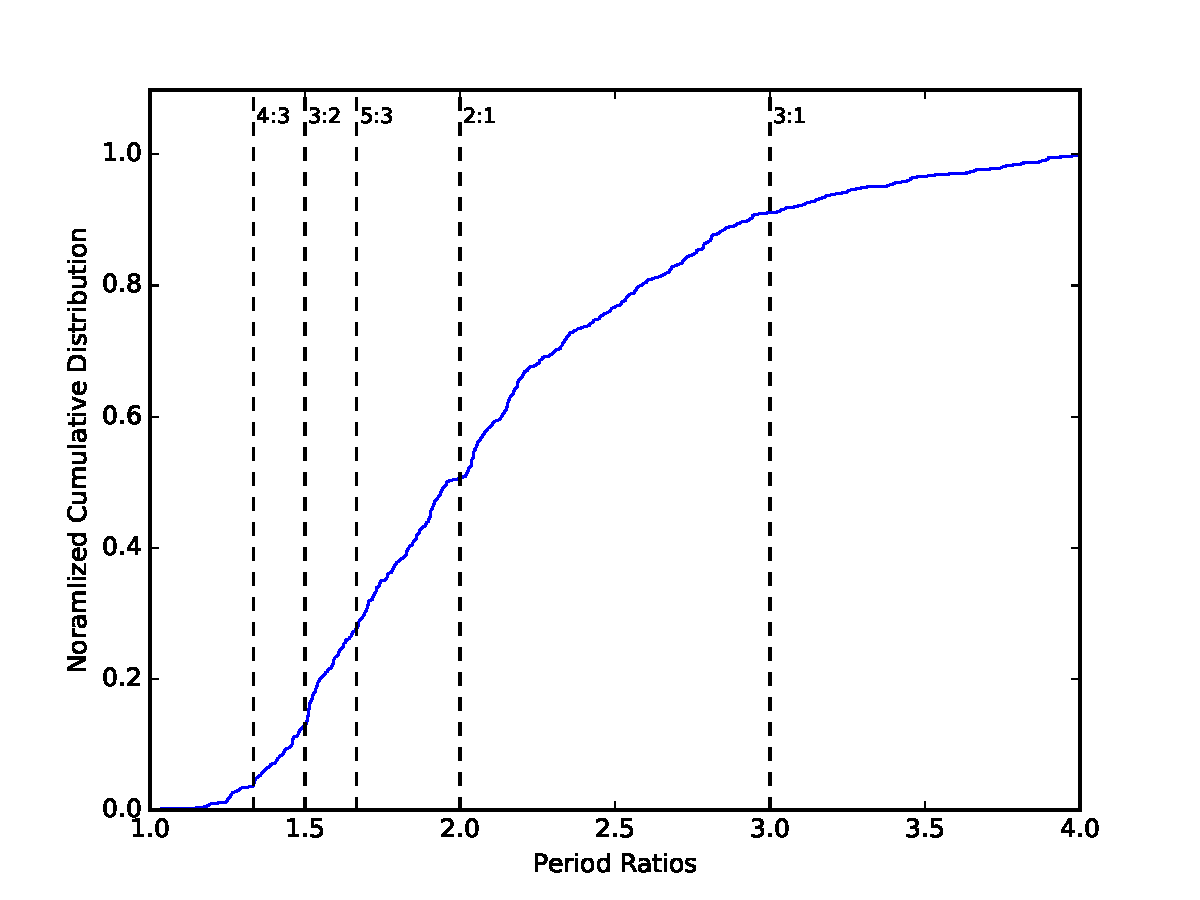
\includegraphics[width=1.00\textwidth]{intro/PeriodRatios}
\caption{
Cumulative distribution of period ratios of neighbouring planets in all known multi-planet systems.
 First and second-order mean motion resonances are displayed as dotted lines, and labelled at the top of the figure. 
 Data from \citet{NASAEA}.}
\label{fig:KepMMR}
\end{figure}

Planets from these statistical pileups are typically a few percent away from exact MMR commensurability, and dissipative mechanisms have been proposed to transport these planets from exact MMR. 
The most popular of these mechanisms are tidal \citep{LithwickWu2012, Batygin2013, Delisle2014}, protoplanetary \citep{Rein2012b, Baruteau2013, Goldreich2014}, and planetesimal \citep{Moore2013, Chatterjee2015}.
The formation implications for each mechanism are different, and no clear consensus has yet emerged.
Chapter~\ref{chap:Tides} critically examines the role of tidal forces in transporting \kep planets from exact MMR to their observed locations, using analytical and numerical means. 

\subsection{Migration}
\label{sec:migration}
Planetary migration is believed to be the most effective way of trapping planets in MMR \citep[e.g.][]{Lee2002}, making it a very important process for planet formation.  
Throughout this thesis (Chapters~\ref{chap:Tides}, \ref{chap:Hermes} and \ref{chap:HD155358}) migration physics is utilized, and presented here are the two primary ways that planets can migrate -- via planetesimals and gas.

\subsubsection{Planetesimal-Driven Migration}
Planetesimals passing through the Hill sphere of a planet will exchange angular momentum via gravity \citep{Ida2000, Kirsh2009}.
If there is an asymmetry to the mass of planetesimals interacting with the planet on its near and far sides, a net force will migrate the planet. 
However, to guarantee a net migration planetesimal orbits must decouple from the planet. 
A massive enough planet (e.g. Jupiter) will directly eject and decouple planetesimals from the system, however if the planet is smaller (e.g. Neptune) planetesimals must decouple by interacting with a neighbouring planet. 
In addition, for sustained migration the planet must constantly encounter fresh, dynamically cold planetesimals \citep{Gomes2004}.  

Since protoplanetary growth is proportional to orbital frequency \citep[e.g.][]{Rafikov2003}, planetesimal disks are most likely to exist in the outer reaches of planetary systems where fewer orbital cycles have occurred. 
In the Solar System, the primordial Kuiper belt is believed to have once been such a planetesimal disk, causing Neptune to migrate outwards into the Kuiper belt and shepherd planetesimals inwards to Jupiter, which subsequently ejected them from the Solar System \citep{Fernandez1984}.
This idea is well supported by observations of the outer Solar System, which show that Pluto, along with a host of smaller bodies, orbit in stable 3:2 MMRs with Neptune \citep{Malhotra1993, Malhotra1995}.

\subsubsection{Gas-Driven migration}
Since the discovery of the first hot Jupiter \citep{Mayor1995}, gas-driven migration is believed to play an important role in shaping exoplanetary systems \citep{Lin1996}.
Whenever a fully-formed planet is embedded in a protoplanetary disk, angular momentum can be exchanged via disk-planet torques \citep{Goldreich1980}.
The result of this exchange is planetary migration, and this scenario is believed to be common to all young planetary systems. 
Gas-driven migration comes in two main flavours -- Type I and Type II. 

Type I migration occurs when low-mass planets are fully embedded in a protoplanetary disk and do not significantly perturb the disk structure \citep{Armitage2010}. 
At particular resonant locations, known as Linblad resonances, density waves are excited due to gravitational interactions between the planet and disk \citep{Goldreich1979}. 
These density waves exchange angular momentum with the planet, and migration occurs when the inner and outer disk interact asymmetrically with the planet \citep{Goldreich1979}.
In general, the direction of Type-I migration tends to be inwards towards the central star \citep{Ward1997}.

Type II migration occurs when high-mass Jovian planets significantly modify the structure of the surrounding protoplanetary disk, opening up a gap. 
This gap locks the planet in place, coupling the migration of the planet to the evolution of the disk \citep{Lin1986}.
The viscous evolution of the disk causes the planet to slowly migrate inwards, at speeds typically one or two orders of magnitude slower than Type-I migration \citep{Ward1997}.

In comparison to planetesimal migration, gas-driven migration is still not well understood. 
In particular, standard calculations of gas-driven migration are too quick by 1-2 orders of magnitude \citep{Lin1986, Tanaka2002}, causing planets to spiral into their central stars before the protoplanetary disk has dispersed.
In contrast to this standard view, recent work \citep{Fung2017} has suggested that planets actually do not migrate that much and tend to be better behaved than originally believed. 
A consensus on migration has yet to be established, but it is clear that some form of migration must occur in the universe due to the large number of planets in or near MMR \citep{Lissauer2011,Fabrycky2014,Steffen2015}.

\subsection{Stability}
\label{sec:stability}
The longterm stability of planetary orbits has been studied for hundreds of years by many famous scientists including Issac Newton, Joseph-Louis Lagrange and Carl Friederich Gauss. 
However, due to the chaotic and non-integrable nature of planetary systems it has been historically difficult to make progress on N-body problems.  
The chaos in planetary systems is caused by overlapping resonances \citep{Chirikov1979, Lecar2001}, resulting in the divergence of near-identical systems on long timescales. 
However, with the aid of computers the equations of motion governing planetary systems can be brute-force integrated into the future or past, allowing scientists to answer fundamental questions that have plagued humans for hundreds of years. 
For example, it is now known that the Solar System is marginally stable \citep{Sussman1988, Laskar1994, Lecar2001}, with Mercury having a 1\% chance of colliding with Venus or the Sun within a couple billion years \citep{Laskar2009}.
It is also now well established that most known multi-planet systems are packed to capacity, and adding additional planets into these systems would result in dynamical instabilities \citep{Fang2013,Pu2015}.

Although most planetary systems cannot be analytically solved, constraints on these systems can still be derived from analytical means.
For example, \citet{Wisdom1980} and \citet{Duncan1989} showed that for small eccentricities in the Restricted 3-Body Problem (R3BP), chaotic orbits (leading to close encounters, collisions and ejections) will occur when the perturber and particle are separated by $\Delta a \le 1.3\mu_p^{2/7}a_p$ (where subscript $p$ indicates the perturber). 
Also associated with the R3BP is the Jacobi constant, which can be used to constrain the chaotic motion of a particle in parameter space. 
For two massive planets, \citet{Gladman1993} showed that orbits are Hill stable if $\Delta a \ge 3.46 R_H$ (where $R_H$ is the mutual Hill radius), forbidding close encounters for all time.

Since the discovery of numerous exoplanetary systems via \kep, longterm stability has become a popular way to constrain orbital parameters \citep{Lissauer2011, Steffen2013, Jontof-Hutter2014, Tamayo2015}. 
If one assumes that an observed system is stable over billions of years, grids of N-body integrations can be used to find stable regions of parameter space, further narrowing the range of valid solutions originally constrained by observations. 
Although this brute-force method is certainly useful, it is not without its costs. 
A 10 billion year integration or the Solar System takes weeks to complete, and due to the chaotic nature of planetary systems hundreds to thousands of realizations must be simulated to acquire statistically rigorous results. 
Chapter~\ref{chap:Stability} shows that using machine learning techniques, accurate predictions of longterm stability can be made. 
These predictions are orders of magnitude faster than direct N-body integrations. 

%%%%%%%%%%%%%%%%%%%%%%%%%%%%%%%%%%%%%%%%%%%%%%%%%
%%%%%%%%%%%%%%%%%%%%%%%%%%%%%%%%%%%%%%%%%%%%%%%%%
%%%%%%%%%%%%%%%%%%%%%%%%%%%%%%%%%%%%%%%%%%%%%%%%%
\section{Numerical Integration}
\subsection{Hamiltonian Dynamics}
The Hamiltonian $\Ham$ encodes the kinetic and potential energy for a system of $N$ bodies. 
In its most basic form, the Hamiltonian is:
\begin{equation}
\Ham  = \sum_{i=0}^{N-1} \frac{\textbf{p}_i^2}{2m_i} - \sum_{i=0}^{N-1} \sum_{j=i+1}^{N-1} \frac{Gm_im_j}{|\textbf{r}_i - \textbf{r}_j|}
\label{eq:H}
\end{equation}
where $\textbf{r}_i$, $\textbf{p}_i$ and $m_i$ are the position, momentum and mass of body $i$, respectively. 
The first term in Equation~\ref{eq:H} sums the kinetic energies of the system, while the second term sums the potential energies of the system.

The coordinates ($\textbf{r}$,$\textbf{p}$) used in Hamiltonian mechanics are canonical, obeying the fundamental Poisson bracket relations:
\begin{equation}
\{\textbf{r}_i, \textbf{r}_j\} = 0, \qquad
\{\textbf{p}_i, \textbf{p}_j\} = 0, \qquad
\{\textbf{r}_i, \textbf{p}_j\} = \delta_{ij}
\end{equation}
where $\delta_{ij}$ is the Kronecker delta. 
A primary benefit of using this Hamiltonian framework is the ease of evolving a system of N-bodies into the future or past via Hamilton's equations:
\begin{align}
\begin{split}
\frac{d\textbf{p}}{dt} &= -\frac{\partial H}{\partial \textbf{r}} \\
\frac{d\textbf{r}}{dt} &= \frac{\partial H}{\partial \textbf{p}} 
\label{eq:Heq}
\end{split}
\end{align}
Numerically this is straightward, with the accuracy of the result being inversely proportional to the size of the timestep, $dt$.
A second benefit is the inherent area preserving or symplectic nature of Hamiltonian systems, with the energy error bound to a finite value (excluding e.g. numerical roundoff errors which grow with time).

Within the context of planetary systems, Equation~\ref{eq:H} can be modified to make integration more efficient.
For example, a single planet will orbit in a Keplerian fashion around a star, determined exactly by the planet's orbital parameters and stellar mass. 
In addition, for multi-planet systems gravitational interactions between planets will occur, perturbing planets off their original Keplerian trajectories.
Thus, a new Hamiltonian can be constructed consisting of a Keplerian term, $\Ham_K$, and Interaction term, $\Ham_I$, according to \citep{Wisdom1991}:
\begin{equation*}
\Ham = \Ham_K + \Ham_I
\end{equation*}
If the planets are well-separated the planet-planet gravitational interactions are relatively small, the system can be numerically integrated by applying Keplerian and Interaction operators in a leapfrog manner:
\begin{equation}
E_{\Ham}(dt) = E_{\Ham_K}(dt/4) \cdot E_{\Ham_I}(dt/2) \cdot E_{\Ham_K}(dt/4)
\label{eq:DKD}
\end{equation}
where $E_{X}(Y)$ represents the evolution of the system under $X$ for time $Y$.
Equation~\ref{eq:DKD} is a second order integration scheme, and is the most popular choice for simulating planetary systems \citep{Wisdom1991}.

\subsection{Coordinate Systems}
As mentioned above, the most efficient way to solve the N-body  problem is to split the Hamiltonian into Keplerian and Interaction components.
In general, the Keplerian and Interaction Hamiltonians take the following form:
\begin{equation}
\Ham_K = \sum_{i=1}^N \frac{\textbf{p}_i^2}{2m_i} - \frac{Gm_0m_i}{\textbf{r}_i}, \qquad
\Ham_I = \sum_{i=1}^{N}\sum_{j=1,j \ne i}^N \frac{Gm_im_j}{|\textbf{r}_i - \textbf{r}_j|}
\label{eq:Hgeneral}
\end{equation}
However, there are numerous ways to perform these splits, with each coordinate system having relative strengths and weaknesses. 
The most popular splittings are are discussed below. 
In all cases $\textbf{r}$ and $\textbf{p}$ represent cartesian position and momenta, respectively, $N$ is the total number of particles, and $M$ is the total mass of the system. 

\subsubsection{Jacobi}
\label{sec:Jacobi}
Carl Jacobi worked out a coordinate system in which the planet positions are measured relative to the centre of mass of all bodies interior to it. 
Since a planet's semi-major axis (and hence position) is dependent upon the mass interior to it by Kepler's 3rd law, in this coordinate system the position of a particle is directly affected by all bodies interior to it. 

The Jacobi position $\textbf{r}^{\prime}$ and momentum $\textbf{p}^{\prime}$ form a canonical set and are related to the cartesian position and momentum according to \citep{SSD1999}:
\begin{equation}
\textbf{r}^{\prime}_i = \textbf{r}_i - \textbf{R}_{i-1}, \qquad
\textbf{p}^{\prime}_i = \frac{\eta_{i-1}}{\eta_i}\textbf{p}_i - \frac{m_i}{\eta_i}\sum_{j=0}^{i-1} \textbf{p}_j
\end{equation}
where $\textbf{R}_i = \frac{1}{\eta_i} \sum_{j=0}^i m_j\textbf{r}_j$ is the centre of mass of all particles interior to body $i$ and $\eta_i = \sum_{j=0}^i m_i$ is the sum of masses interior to body $i$.
For the special case of $i=0$:
\begin{equation}
\textbf{r}^{\prime}_0 = \textbf{R}_{N}, \qquad
\textbf{p}^{\prime}_0 = \sum_{j=0}^{N} \textbf{p}_j
\end{equation}
The inverse transformations from Jacobi coordinates to cartesian coordinates can be found in Chapter 9.5 of \citet{SSD1999}.

The benefit of Jacobi coordinates is that the kinetic terms remain a sum of squares \citep{Plummer1918}, making numerical integration a straightforward process according to Equation~\ref{eq:DKD}. 
In addition, these coordinates solve the Two Body and Restricted Three Body Problems exactly. 
However, the primary disadvantage is that a clear ordering of bodies is required for efficient integration in Jacobi coordinates. 
For example, orbits within a planetesimal disk frequently cross, and there is no straightforward and (computationally) cheap way to order these bodies. 

\subsubsection{Democratic Heliocentric}
\label{sec:DH}
In this coordinate system positions $\textbf{Q}$ and momenta $\textbf{P}$ form a canonical set with $\textbf{Q}$ measured relative to the central body and $\textbf{P}$ measuring barycentric momenta.
These coordinates are related to the cartesian position and momenta according to \citep{Duncan1998}:
\begin{equation}
\textbf{Q}_i = \textbf{r}_i - \textbf{r}_0, \qquad
\textbf{P}_i = \textbf{p}_i - \frac{m_i}{M}\sum_{j=0}^N \textbf{p}_j
\end{equation}
For the special case of $i=0$:
\begin{equation}
\textbf{Q}_0 = \frac{1}{M} \sum_{j=0}^N m_j \textbf{r}_j, \qquad
\textbf{P}_0 = \sum_{j=0}^{N} \textbf{p}_j
\end{equation}

The benefit of Democratic Heliocentric coordinates is that positions are not dependent upon other bodies (unlike Jacobi coordinates) and are thus conceptually easier to understand. 
However, these coordinates do not solve the Two Body Problem or Restricted Three Body Problems exactly. 
In addition, $\Ham_K$ cannot be cleanly written as shown in Equation~\ref{eq:Hgeneral} due to several cross terms that arise when substituting $\textbf{Q}$ and \textbf{P}.
However, this problem can be rectified by transferring these cross terms into an additional Jump Hamiltonian:
\begin{equation}
\Ham_J = \frac{1}{2m_0} \left|\sum_{i=1}^N \textbf{P}_i\right|^2
\end{equation}
Therefore, the evolution of $\Ham$ in Equation~\ref{eq:DKD} must be modified to include an additional evolution operator under the Jump Hamiltonian, $E_{\Ham_J}$.
Note that since $\{\Ham_J, \Ham_I\} = 0$, the ordering of $E_{\Ham_I}$ and $E_{\Ham_J}$ does not matter. 

\subsubsection{WHDS}
The WHDS is a modification of the Democratic Heliocentric mapping and splits the kinetic energy slightly differently. 
The canonical coordinates $\textbf{Q}$ and $\textbf{P}$ have the same form, but the Keplerian, Interaction and Jump steps are now \citep{Laskar1995, Wisdom2006, Hernandez2016}:
\begin{align}
\begin{split}
\Ham_K &= \sum_{i=1}^N \frac{\textbf{P}_i^2}{2\mu_i} - \frac{G(m_0 + m_i)\mu_i}{\textbf{Q}_i} \\
\Ham_I &= \sum_{i=1}^{N}\sum_{j=1,j \ne i}^N \frac{Gm_im_j}{|\textbf{Q}_i - \textbf{Q}_j|} \\
\Ham_J &= \sum_{i=1}^{N}\sum_{j=1,j \ne i}^N \frac{\textbf{P}_i \cdot \textbf{P}_j}{m_0}
\end{split}
\end{align}
where $\mu \equiv m_im_0/(m_0 + m_i)$.

The benefit of these coordinates is that, unlike Democratic Heliocentric coordinates, the Two Body and Restricted Three Body Problems are now solved exactly. 
In addition, (like Democratic Heliocentric coordinates) a particle's position are not dependent upon any other bodies. 
One price to pay for these benefits is that $\{\Ham_J, \Ham_I\} \ne 0$, and in Equation~\ref{eq:DKD} $E_{\Ham_J}$ must be exactly nestled in between the $E_{\Ham_K}$ and $E_{\Ham_I}$ operators.
In addition, the standard symplectic correctors of \citet{Wisdom2006} cannot be used in this coordinate system, however other correctors may be possible to construct. 

\subsection{Integrator Types}
\label{sec:inttypes}
The three main classes of N-body integrators are symplectic, non-symplectic and hybrid. 
Symplectic integrators employ a fixed timestep, bounded energy error (excepting bias and roundoff errors which grow with time) and fast integration time.
These integrators are best suited for well-separated bodies where $\Ham_I \ll \Ham_k$, otherwise the energy error increases dramatically or the timestep must be changed, both of which break symplecticity. 
The most popular symplectic integrator is the Wisdom-Holman mapping \citep{Wisdom1991}.

Non-symplectic integrators do not require a fixed timestep and do not have a bounded energy error over time. 
However, these integrators can employ very accurate and precise numerical convergence schemes, for example the Burlish-Stoer or predictor-corrector algorithms \citep{Press2002}.
As a result, non-symplectic integrators are typically more accurate but slower than their symplectic counterparts, and can solve most classes of planetary physics problems. 
A popular non-symplectic integrator is \ias \citep{Rein2015a}.

Hybrid integrators typically mix the symplectic and non-symplectic schemes, applying the symplectic component on bodies that are distant and non-symplectic component on bodies that are close. 
However, there are hybrid schemes that purely rely on symplectic principles \citep[e.g.][]{Duncan1998}.
As a result, hybrid integrators are often an optimal balance between speed and accuracy, especially for problems involving numerous close encounters. 
The most popular hybrid integrator is \mercury \citep{Chambers1999}.
Chapter~\ref{chap:Hermes} presents \hermes, a new hybrid integrator designed for the migration of planets embedded in planetesimal disks. 

%%%%%%%%%%%%%%%%%%%%%%%%%%%%%%%%%%%%%%%%%%%%%%%%%
%%%%%%%%%%%%%%%%%%%%%%%%%%%%%%%%%%%%%%%%%%%%%%%%%
%%%%%%%%%%%%%%%%%%%%%%%%%%%%%%%%%%%%%%%%%%%%%%%%%
\section{This Work}
The work presented in this thesis focusses on the statistics, formation and stability of planetary systems. 
Chapter~\ref{chap:Stats} deals with a statistical analysis of \kep planets while incorporating the large radius errors present in the \kep data. 
As mentioned in Section~\ref{sec:stats}, the analyses by \citet{Fressin2013} and \citet{Petigura2013} ignored these large errors in planetary radius, affecting their calculations of planet occurrence.

Chapter~\ref{chap:Tides} investigates the role of tides in transporting planets from exact MMR commensurability to a few percent wide. 
From Figure~\ref{fig:KepMMR}, an excess of planets is seen wide of the 3:2 MMR and 2:1 MMR. 
As mentioned in Section~\ref{sec:MMR}, it is believed that these planets were originally trapped in MMR and some mechanism transported them a few percent wide. 
Other studies have investigated the role of tides in transporting planets from MMR using analytical \citep{Lee2013, Delisle2014} means, but no one has yet investigated this question numerically.
Although computationally expensive, N-body simulations are very accurate and avoid approximations. 

Chapter~\ref{chap:Hermes} presents \hermes, a hybrid integrator for simulating planetesimal migration, built from \ias \citep{Rein2015a} and \whfast \citep{Rein2015b}. 
An adaptive switching radius is also available for \hermes, optimizing the close-encounter boundary and ensuring accurate integration.
In addition, \hermes is compared to other popular hybrid integrators. 
As outlined in Section~\ref{sec:inttypes}, hybrid integrators are best for simulating planets embedded in planetesimal disks, which I plan to investigate in future works (Chapter~\ref{sec:Future}). 

Chapter~\ref{chap:Stability} investigates the role of machine learning in predicting longterm planet stability. 
As stated in Section~\ref{sec:stability}, due to the non-integrable and chaotic nature of multi-planet systems, classification of planetary stability is difficult without performing numerous costly N-body simulations. 
However, using information from the initial conditions and early evolution, we show that a trained machine learning algorithm can accurately predict whether a planetary system will be longterm stable.  
This tool is useful to the scientific community due to its speed in classifying systems over direct N-body integrations.  

Finally, in Chapter~\ref{chap:HD155358} the HD155358 system is analyzed, which consists of two Jovian-sized planets orbiting a few percent from the 2:1 MMR around a $0.92M_{\odot}$ star. 
Radial velocity data for HD155358 was previously collected and analyzed by \citet{Robertson2012}, but they did not account for gravitational planet-planet interactions when deriving the orbital parameters.
As mentioned in Section~\ref{sec:RV}, neglecting planet-planet interactions in the orbital fit is only valid when the interactions are weak. 
We derive new orbital parameters and find a high likelihood that the planets are in MMR.
In addition, as mentioned in Section~\ref{sec:migration} planets near MMR are likely to have formed via migration, and we analyze both the formation and longterm stability of the system. 

\chapter[Statistical Reconstruction of Kepler Planets]{A Statistical Reconstruction of the Planet Population around Kepler Solar-Type Stars}
\label{chap:Stats}

\section{Chapter Overview}
	\begin{center}
	\begin{minipage}[c]{4.75in}
	The work, tables, and figures from this Chapter are based off the following publication:\\
	
	Ari Silburt, Eric Gaidos, Yanqin Wu\\
	The Astrophysical Journal, Volume 799, Issue 2 - article id. 180, 12 pp., 2015 \citep{Silburt2015}.
	\vspace{2em}
	\end{minipage}
	\end{center}

Using the \citet{Ramirez2014} catalog of (candidate) planets detected by the
NASA {\it Kepler} mission, we reconstruct the intrinsic occurrence of Earth- to
Neptune-size planets and their distributions with radius and orbital
period.  We analyze 76,711 solar-type ($0.8<R_*/R_{\odot}<1.2 $) stars with 430 planets 
on 20-200~d orbits, excluding close-in planets that may have been affected by
the proximity to the host star.  Our analysis considers errors in
planet radii and includes an ``iterative simulation'' technique that
does not bin the data.  We find a radius distribution that peaks at
2-2.8 Earth radii, with lower numbers of smaller and larger planets.
These planets are uniformly distributed with logarithmic period, and
the mean number of such planets per star is $0.46 \pm 0.03$.  The
occurrence is $\sim 0.66$ if planets interior to 20~d are included.  We
estimate the occurrence of Earth-size planets in the ``habitable zone"
as $6.4^{+3.4}_{-1.1} \%$.  Our results largely agree with those of \cite{Petigura2013}, 
although we find a higher occurrence of 2.8--4
Earth-radii planets. The reasons for this excess are the inclusion of errors in 
planet radius, updated \cite{Huber2014} stellar parameters, and likely also the 
exclusion of planets which may have been affected by proximity to the host star.

\section{Introduction}
\label{sec:introduction}

Anaximander of Miletus proposed that there were many Earth-like worlds
\footnote{{\it Dissertation on the Philosophy of Aristotle, in which
    his Principal Physical and Metaphysical Dogmas are Unfolded},
  transl. by T. Taylor, London, 1812}.  In the twenty five centuries
since the Ionian philosopher's speculation, we have seen an
accelerating convergence towards an answer: many if not most stars
have planets, Earth-sized (and presumably rocky) bodies are more 
common than Jupiter-sized gaseous bodies, and
some Earth-sized planets are on orbits in the so-called
``habitable zones'' of their stars \citep{Schneider2011}. The most recent advances in this
field have come from data collected by the \kep{} transiting-planet
mission \citep{Borucki2010}.  Four years of observations of a $\sim
100$ sq. deg. field have led to the identification thus far
of 4234 confirmed or candidate transiting planets, about 84\% of the
candidates appear to be smaller than Neptune (3.88\rearth{}) \citep{NASAEA}.

Beyond simple human curiosity about the prevalence of Earth-like
planets and possibility of life elsewhere, planet statistics provide
an important test of planet formation models \citep[e.g.][]{Benz2014}.
For example, the distribution of planets with respect to orbital
period and mean motion resonances test models of planet formation and
early migration \citep[e.g.,][]{HansenMurray,Baruteau2013}.  Planet
radius and period distributions can be combined to reconstruct the
distribution of solid mass in disks
\citep[e.g.,][]{Chiang2013,Raymond2014}.

There have been many previous studies that use the \kep{} data to
infer the intrinsic population of planets around \kep{} target stars,
or subsets of those stars
\citep[e.g.][]{Catanzarite,Youdin,Traub2012,Howard2012,Fressin2013,
  Dressing2013,Gaidos2013,Dong2013,Kopparapu2013b,Petigura2013}.
These works differ in their samples and methods, but are broadly
consistent in estimating that the occurrence of planets per star on orbits of days to months
to be of order unity.  Some of these works have estimated \ee{}, the
occurence of Earth-size planets in a circumstellar ``habitable zone''
(where stellar irradiation is similar to the solar constant), and find
that \ee{} is of order tens of percent.  Of particular interest to us
is the work of \citet[][hereafter PHM13]{Petigura2013} who performed
an independent analysis of the \kep{} photometric lightcurves, both
identifying candidate planet transits and determining the detection
efficiency by injecting synthetic transit signals into \kep{}
lightcurves and recovering them.  Among the salient conclusions from
PHM13 are that the distribution of planets peaks at a radius of
2--2.8\rearth{} and that, \ee{} is about 22\% (using a liberal
definition of the habitable zone).

We identify two reasons to revisit the derivation of the \kep{} planet
population. Firstly, we want to more fully account for the
uncertainties and biases in the \kep{} data and related observations
of the target stars.  Secondly, we wish to consider a ``primordial''
planet population, and restrict our analysis to planets far enough
from their host stars such that their properties have not been altered by
proximity since their formation.

Precise statements on the occurrence of planets requires rigorous
statistical methods, full accounting of errors, and adequate
assessment of potential biases.  First, while the overall rate of
``false positives'' among \kep{} candidate planets appears to be low
\citep{Morton2011,Fressin2013}, it is not uniform across all
  periods and all sizes \citep{Santerne2013}.  Second, determination
of planet occurrence from transit surveys requires accurate estimates
of detection efficiency (also known as ``completeness''), which depends on the
parameters (i.e. density and/or radius) of not only the planet host
stars but of the entire target catalog. The parameters of \kep{} stars
were first determined by combining multi-wavelength photometry,
stellar models, and Bayesian inferrence \citep{Brown2011}.  Colors of
solar-type stars depend only weakly on gravity and metallicity, and
parameter values based on photometry have large random and systematic
errors in both effective temperature \citep{Pinsonneault2012}, gravity
and luminosity class \citep{Mann2012}.  Spectroscopy, asteroseismology,
and improved stellar models have yielded more reliable parameters 
\citep{Huber2014}, especially for \kep{} planet-hosting stars 
(\kep{} Objects of Interest or KOIs).  Nevertheless, 70\% of all stars in the
\citet{Huber2014} catalog have assigned parameters based on KIC
photometry; the median upper and lower fractional errors in stellar
radius among these solar-type stars is 40\% and 10\%, respectively. Because
the estimated radius of a planet detected by transit depends on the
stellar radius, and the probability of transit depends on stellar
density, these errors need to be taken into account when computing
occurrence rates.  Errors in luminosity also affect the certainty with
which a planet can be assigned to a habitable zone described by a
range of stellar irradiance \citep{Gaidos2013,Mann2013}.

Third, biases, if uncorrected or unaccounted for, will distort our 
perspective on planet populations.  
%Perhaps the most insidious is detection bias, where the properties of stars with detected planets are statistically different from that of the overall target population.  The assumption that there is no such difference can lead to erroneous conclusions about the properties of stars with planets and occurrence rates.  
\citet{Mann2012} found that up to $96\%$ of
the reddest \kep{} target stars are giants, even though virtually all
red KOI hosts are dwarfs for the simple reason that it is extremely
difficult to detect a transiting planet around a giant star.  They
showed that dilution of the target catalog by giants had led to an
underestimate of the occurrence rate and an incorrect claim that M
dwarf hosts of detected planets are redder and thus more metal-rich
than those without detected planets.

\citet{GaidosMann2013} showed that because the \kep{} target catalog
is essentially magnitude-limited, Malmquist bias combined with
uncertainties in stellar parameters means that stellar distances are
underestimated and many stars are likely to be more luminous, evolved,
and larger than their nominal values.  Follow-up observations and
analysis thus far seem to confirm this
\citep[e.g.][]{Bastien2014,Everett2013,Verner2011}.  Because
transiting planet radius scales with increasing stellar radius, this means that
planet radii are underestimated.  Moreover, the rate of planet
detection decreases with increasing stellar radius or density, thus
for a given planet radius, the detection rate is overestimated and
thus the occurrence is underestimated.  Detection bias again means
that any estimate of this effect based on the host stars of transiting
planets is an {\it underestimate}: the effect will be greater among
stars in the overall target catalog.  Another bias is Eddington bias:
scatter by error from more populated regions of parameter space into
less populated regions will produces the opposite effect,
i.e. occurrence will be overestimated \citep{GaidosMann2013}.

Previous analyses of the \kep{} planet population have sometimes not taken
these errors or biases into account, and instead have considered only
Poisson (counting) statistics \citep[e.g.][]{Petigura2013,Howard2012}.
Finally, many analyses
were performed by binning the data into discrete bins of planet radius $R_p$
and orbital period $P$.  While simple and readily explicable, the binning
method runs the risk of masking details of a distribution, especially
that of radius, which may be important for testing theoretical
models.

In this Chapter we consider a ``primordial'' population of
planets, as opposed to one that has evolved under the influence of the
host star. Effects of the latter, including tidal heating
\citep{Jackson2008}, atmospheric escape \citep{Tian2005}, ohmic heating
\citep{Batygin2011}, and impact erosion \citep{Marcus2009}, act with
an efficiency that is inversely proportional to the distance to the
host star. In particular, \citet{Owen2013} proposed that
photoevaporation by stellar X-ray and ultraviolet irradiation have effectively removed
the hydrogen envelopes of close-in planets ($P \leq 10$~d), leading
to the observed paucity of super-Earth sized planets in that
neighbourhood.  This process was also investigated for a few \kep{}
systems by \citet{Lopez2012}. Regardless of the mechanism, the
distinctiveness of the $P< 20$~d and $P>20$~d populations \citep[see,
e.g.][]{Youdin} suggests that any analysis treat these separately.  In
this study, we focus exclusively on the latter population as we
believe it is more likely to represent the ``primordial'' state.  On
the other hand, because of \kep{}'s low efficiency at detecting
long-period planets (see \S \ref{sec:completeness}), we are forced to
limit our consideration to planets with $P<200$d.

Practical reasons also limit the range of planet radius $R_p$
considered.  Although \kep{} can readily detect a transiting giant
planet, the occurrence of these objects is indubitably much lower than
that of smaller planets.  The distribution with planet radius falls to
a very low level beyond Neptune-size objects: only 8\% of \kep{}
candidate planets have nominal radii $>8$\rearth{}, and the
false-positive rate increases as well \citep{Santerne2012,Colon2012}.
Conversely, \kep{} can detect planets smaller than 1\rearth{} for only
a tiny fraction of stars, mostly M dwarfs.  For these reasons we
restrict our analysis to a radius range of 1--4\rearth{} over which
statistically rigorous analyses can be performed. 

In this Chapter, we infer the intrinsic distribution of planets
with $20<P<200$~d (equivalent to 0.16--0.67~AU) and
$1 R_\oplus < R_p < 4R_\oplus$ around solar-type stars as
observed by \kep{} over
its entire mission (Quarters 1--16).  This analysis includes the
effects of errors in stellar and planet radius, and takes into account
some of the biases that may affect previous works.  We introduce a
method of iterative simulation to determine the radius distribution of
planets without resorting to binning.  We compare our results with
those of PHM13 and also carry out a detailed comparison of the two
methods to understand the source of any discrepancies.  Finally, we use our
simulations to assess the effect of systematic bias, namely an overall 
underestimate of stellar radius, on
inferences of a planet population from the \kep{} catalog.

%%%%%%%%%%%%%%%%%%%%%%%%%%%%%%%%%%%%%%%%%%%%%%%%%%%%%%%%%%%%%%
\section{Methods}
\label{sec:methods}
\subsection{Catalogs of Stars and Planets}
\label{sec:catalogs}
We construct a stellar sample from the \cite{Huber2014} catalog of
196,468 stars observed during the \kep{} mission (Quarters 1--16),
selecting ``Sun-like'' stars with radii $0.8R_{\odot}<R_*<1.2R_{\odot}$. We
restrict the sample to stars with a \kep{} magnitude $K_{p}<15.5$ to
avoid faint stars with uncertain properties and noisy lightcurves.
This leaves a sample of 76,711 solar-type stars, hereafter known as
the ``Solar76k'' sample.  Our planet sample is constructed from the 26
February 2014 version of the KOI catalog \citep{Ramirez2014}.  Planet
and stellar parameters are updated with values from \cite{Huber2014}
where available.  In addition to the cuts made on our stellar sample
we also require $20<P<200$ d, $0.5R_{\oplus}<R_p<6R_{\oplus}$ and
SNR$>$12. Although we are only interested in the occurrence of planets 
$1R_{\oplus}<R_p<4R_{\oplus}$, we use a larger radius range for our analysis 
since these planets have a non-zero probability of being in our region of 
interest after accounting for radius errors (\S\ref{sec:plerr}).
This leaves us with 430 candidate planets, hereafter known
as the ``430KOI'' sample. We also construct a second planet sample
(used only in \S\ref{sec:intperiod}) using the same cuts above
except relaxing the period restriction to $5<P<200$.  This leaves us with
1052 KOIs, hereafter known as the ``1052KOI'' sample.

To ease comparison with PHM13, we retrieve their vetted sample of
603 planet candidates that fall within $5<P<100$~d. We update the stellar
parameters where possible, using \citet{Huber2014}.  We hereafter
refer to this planet sample as the ``603PHM'' sample.

\subsection{Simulated Planet Detections}
\label{sec:geneq}

Our simulator synthesizes single planet-star pairs\footnote{ We
  ignore the occurrence of multiple systems and assume that each
  planet has an independent occurrence.},  drawing stars from one of
the catalogs described above, and planet parameters from a large
``master'' population as we describe in \S \ref{sec:plerr}.  We calculate whether each
planet transits its host star in a probabilistic manner, and then determine
whether \kep{} could have detected it.  We compare the
properties of these simulated detections with the observed candidate \kep{}
planets, and modify the master population using two different
techniques: iterative Monte Carlo Markov Chain (MCMC) and Iterative Simulation
(IS).  In implementing our simulations we make two critical
assumptions. First, that the orbital periods and radii of \kep{}
planets (as well as orbital eccentricities), are independently
distributed, i.e. the occurrence is a separable function of period and
radius:
\begin{equation}
{{d^2 N}\over{{d\log P \, d\log R}}} = p(P) r(R)\, ,
\label{eq:assumption}
\end{equation}
where $p$ and $r$ are some yet-to-be-determined functions, and  
$N$ is the total number of planets. 
Second, we assume that these distributions do not vary over the range
of stellar parameters considered.  We discuss these assumptions in \S
\ref{sec:sensitivity}.  In this study, we further specify that the
  period distribution is a power-law:
\begin{equation}
\frac{dN}{d log P} = C P^{\alpha}\, ,
\label{eq:P}
\end{equation}
where $C$ is a normalization constant.

The geometric probability that a planet transits its host star is
\citep{Winn},
\begin{equation}
\label{eqn.probtransit}
p = \frac{R_*}{a}\frac{1+e \sin \omega}{1-e^2},
\end{equation}
where $a$ is the semimajor axis, $e$ the orbital eccentricity, and
$\omega$ the argument of periastron.  While $a$ can be calculated from
$P$ and the estimated mass of the host star, the orbital eccentricity
of \kep{} planets are unknown and must be estimated statistically.
Assuming a Rayleigh distribution with
  dispersion $\sigma_e$, \citet{Moorhead2011} estimated $\sigma_e =
0.2$ by studying the distribution of transit durations. This
  is likely affected by uncertain stellar radii and may be an
  overestimate. TTV studies have led to much smaller eccentricity
  dispersion ($\sigma_e \sim$ a few percent), at least in multiple
  planet systems \citep{WuLithwick,HaddenLithwick}. Here, we choose
$\sigma_e = 0.18$ and show that our results are not sensitive to the
exact value of $\sigma_e$ (\S \ref{sec:sensitivity}). 
The underlying distribution of $\omega$ can be safely assumed to be
uniform over [0,$2\pi$].  
Integrating $p$ over the distributions of $e$ and $\omega$,
Eq.~\ref{eqn.probtransit} becomes $p = p_0 R_*/a$, with
$p_0=1.073$.  As in previous works, we require that at least three
transits have been observed. 
We scale every transit probability by $(1/p_0)(a/R_*)_{max}$, 
the inverse of the max transit probability. Since transiting planets
occur only for $<5$ degrees of inclination, this scaling is used to speed up
the rate of transiting planets. Otherwise, we would have to wait long 
periods of time in order acquire the large numbers of transiting planets we require
to conduct this analysis. 

We now proceed to assign a transit duration, $T$, to a given
transiting planet. We follow the procedure of \citet{Gaidos2013} 
by setting
\begin{equation}
\label{eq:T_IS}
T = \tau^{2/3}P^{1/3}\Delta\, ,
\end{equation}
where $\tau = 2\sqrt{R_*^3/(\pi G M_*)}$ is the stellar free-fall
time, $G$ the gravitational constant, $M_*$ the stellar mass, and
\begin{equation}
\label{eqn.delta}
\Delta = \frac{\sqrt{(1-e^2)(1-b^2)}}{1 + e \cos \omega}\, , 
\end{equation}
with $b$ being the impact parameter. For $a \gg R_*$, the impact
parameter $b$ is uniformly distributed in the range [0,1].
We then calculate $dN/d\Delta$, the likelihood of drawing a
given $\Delta$, or rather, its cumulative distribution,
$\overline{N(\Delta)} \equiv \overline{\int_0^\Delta
{dN}\over{d\Delta'}}d\Delta'$, with the overbar indicating 
marginalization over $e$ and $\omega$. 
Using the chain rule, we find
\begin{equation}
\label{eq:delta1}
%\overline
{\frac{dN}{d\Delta}} d\Delta = 
%\overline
{\frac{dN}{db}}
%\overline
{\frac{db}{d\Delta}} d\Delta = 
%\overline
{\frac{db}{d\Delta}} d\Delta,
\end{equation}
where we have used the fact that $dN/db = 1$ (i.e. $b$ is uniformly distributed) 
for transiting systems.
As a result, $\overline{N(\Delta)} = \overline{b} = \overline{\int_0^\Delta
  {{db}\over{d\Delta'}} d\Delta'}$.  Inverting
Eqn.~\ref{eqn.delta} then yields:
\begin{equation}
\overline{N(\Delta)} = \int_0^1 \eta(e) de \int_0^{2\pi} \sqrt{1 -
  \frac{\Delta^2\left(1 + e \cos \omega\right)^2}{\left(1-e^2\right)}}d\omega, 
\end{equation}
where $\eta(e)$ is the assumed eccentricity distribution.  

We also need to assign a radius to each trial planet: this
process differs between our MCMC and IS methods and is described in
their respective sections. Moreover, in comparing the radius
distribution of trial planets to the observations, we must take into
account significant uncertanties in the radius of KOIs.
% (This is not
%the case for the orbital periods, which are precisely established).
We describe how we do this in the next section.

Our detection criterion is based on a comparison
between the transit signal, $(R_p/R_*)^2$, and the
effective noise over the transit duration.  \citet{Fressin2013}
established that at signal-to-noise SNR $>12$ the false-positive rate
among \kep{} KOIs is very low.  PHM13 used this criterion for their
analysis and we follow suit.  Noise in \kep{}
lightcurves is derived from photon (shot) noise, measurement error 
 (e.g. pointing error and instrument noise)
and stellar variability \citep{Koch2010}.  The \kep{} team encapsulates
the total noise of each star into quarterly transit durations of 
3-hr, 6-hr and 12-hr, known as ``CDPP''
\citep[Combined Differential Photometric Precision,][]{Christiansen2012} 
values. For a given star in a given quarter, we generate the appropriate
noise for transit duration $T$, by interpolating among the various
CDPP values using a power-law relation.  Because sources of noise
(e.g., stellar variability) are not neccesarily ``white'', 
the power-law index can and often does depart from -0.5, the
white noise value.

 We then calculate the total SNR of a model star-planet pair as
\begin{equation}
SNR = \left(\frac{R_p}{R_*}\right)^2 \left[\sum\limits_{j=1}^{16}
\frac{n_j}{\left({\rm CDPP}_j\right)^2} \right]^{1/2},
\label{eq:SNR}
\end{equation}
where $n_j$ is the number of transits in quarter $j$, and CDPP$_j$ is
the interpolated CDPP value for that quarter.  $n_j$ is found by
first assigning a randomly drawn phase for each planet, and then counting 
the number of transits in each quarter.  The system is 
proclaimed detectable if SNR $> 12$. The SNR threshold does
not account for noise that is non-Gaussian or non-stationary on a
timescale shorter than one observing quarter (90~d).  However, the
conservative requirement that SNR $> 12$ for detection
partially addresses this limitation and we consider the possible impact 
of this simplification in \S\ref{sec:petcomp} when we compare our analysis 
to PHM13. Other non-stationary effects unaccounted for in Eq.~\ref{eq:SNR}
include thermal settling events, sudden pixel sensitivity drop offs, and cosmic rays.  
Eq.~\ref{eq:SNR} also does not account for gaps in the data.

\subsection{Uncertainties in Planet Radii}
\label{sec:plerr}

As described in \S\ref{sec:introduction}, there are significant
uncertainties in the radii of most KOIs (median uncertainty = 33\%),
primarily due to our limited knowledge of the host star.  For example,
this means that there is a non-negligible chance that a planet
with a cataloged radius value of $R_p = 2.5$\rearth{}
is actually Earth-sized or Neptune-sized.  To clarify, we are not 
addressing the issue that some dwarf stars are actually giants 
(which is addressed in Section~\ref{sec:radiusdist}
when we consider that all stars are 25$\%$ larger). Instead,   
we are assuming that all claimed dwarf stars are truly dwarfs, and are 
accounting for the fact that the exact radii 
of these stars are still uncertain (on average) to $\sim 30 \%$. 

It is important that
uncertainties of such magnitude be considered, and we do this by
replacing each nominal radius by a distribution of radii governed by
Bayesian statistics.  The probability that a planet with a reported 
radius $R$ actually has a true radius
$R'$ is given by $p(R'|R) = q(R|R')r(R')$, where $r(R')$ is a
normalized prior and is the probability that a planet of radius 
$R'$ (with same period $P$) would be detected by \kep{} around a given 
star. Put another way, $r(R')$ is essentially the survey completeness 
(\S\ref{sec:completeness}) of planet $R'$ (having period $P$) with 
respect to the entire Solar76k catalog. 

In our treatment, we assume that errors in $R_*$ and hence $R_p$ are
normally distributed.  This means that
$q(R|R') = q(R'|R)$ because the Gaussian only depends on the square of
the difference $R-R'$.  We also assume that errors in stellar radius are 
uncorrelated.  This latter assumption means that a planet
with a radius that has been over/underestimated would, on average,
produce a weaker/stronger transit signal among the ensemble of target
stars and that such a planet would become less/more detectable.
If errors in $R_*$ were exactly correlated, then errors in $R_p$ would be
unaffected by considerations of detection; if all stars are smaller
then their planets will also be smaller but by the same proportion,
and thus produce transit signals of the same depth.

Provided these assumptions hold, a planet cannot be arbitrarily small,
even if the errors in radius are large, because it would never have
been detected in the first place. The $r(R')$ factor accounts for this 
fact. Our prescription for handling radius errors also accounts for 
the fact that the cataloged radius is more 
likely to be an underestimate, rather than an overestimate, of the 
true radius. This effect becomes most pronounced among KOIs with 
small cataloged radii and large uncertainty. For these cases the result is an error
distribution that is no longer a Gaussian but is strongly asymmetric,
with a cutoff just below the cataloged radius and an extended tail to
larger radii. An example probability distribution in radius
for KOI-1338.01 (solid) and KOI-1925.01 (dotted) are shown in 
Figure~\ref{fig:prob}. The vertical red lines represents the
catalogued radius values. As seen in Figure~\ref{fig:prob}, the 
most likely radius differs from the catalog value.

\begin{figure}[h]
\centerline{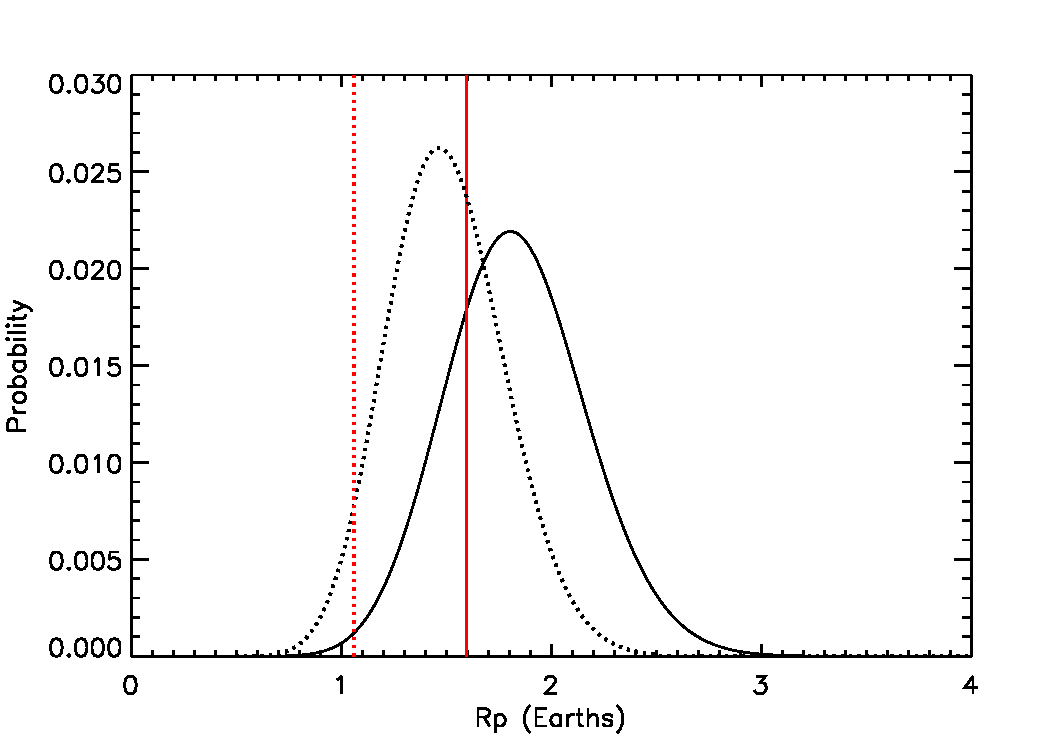
\includegraphics[scale=0.55]{chap2/prob_dist.pdf}}
\caption{Example probability distributions in radius for KOI-1338.01 (solid) and 
	KOI-1925.01 (dotted). The probability distributions are shown in black, 
	while the vertical red lines represents the quoted radius 
	values. As seen in the figure, the most likely radius value can 
	differ from the catalogue value, and sometimes significantly so.}
\label{fig:prob}
\end{figure}

We implement radius errors into our analysis by replacing each KOI with a probability
distribution function (PDF) that is the product of a Gaussian times a
prior detection function which is the fraction of stars around which
the planet would be detected (i.e. completeness). We represent the 
PDF by a large number of Monte Carlo planets drawn from a Gaussian 
distribution with mean equal to the nominal value of $R_P$ and 
standard deviation equal to the cataloged error. We calculate the 
fraction of stars $F$ around which each
Monte Carlo planet could be detected.  

We then compute a normalized
CDF of $F$ with $R_p$ for each Monte Carlo set.  We can then draw a
radius value from each corrected error distribution by comparing the
CDF to a unit random deviate.  We create a ``master'' radius
distribution by randomly drawing 2 million values from all of these
distributions according to their CDFs.  We use this distribution to
represent the inferred radius distribution of observed candidate
planets after errors have been accounted for.

\subsection{Monte Carlo Markov Chain}
\label{sec:mcmc}
We implement the Monte Carlo Markov Chain according to the 
algorithm by \citet{Gelman92}.
We discretize the radius-period plane into 16 bins, 4 period bins
equally spaced in $\log P$ ($P$ = [20--40, 40--80, 80--160, 160--200]
~d) and 4 radius bins equally spaced in $\log R$ (1--1.4\rearth{},
1.4--2\rearth{}, 2-2-.8\rearth{}, 2.8--4\rearth{}). We parametrize the
planet population by a set of 4 parameters: $\alpha$ (from
Eq.\ref{eq:P}), and $\kappa_1, \kappa_2, \kappa_3$, where the
latter 3 parameters are the relative numbers of planets in the first
3 radius bins to the last bin. For each set of
parameters, we generate a mock catalog by simulating $10^5$
transiting pairs around a given stellar sample (\S \ref{sec:geneq})
while properly taking into account errors in planet radius (\S
\ref{sec:plerr}).  We then compare our mock population against
the 430KOI sample by first binning the KOIs in the same manner and then removing 
a portion from each bin to account for false positives 
\citep[Table 1 from][]{Fressin2013}. We then scale our mock catalog 
down from $10^5$ to match the total number of remaining KOIs. 
The goodness of fit is measured by comparing the simulated number of
planets in each of the 16 bins, $S_i$, versus that of the
observed, $D_i$,
\begin{equation}
\chi^2=\sum\limits_{i=1}^{16} \frac{({\rm D}_i - {\rm S}_i)^2}{{\rm S}_i}, 
\end{equation}
Here, we have assumed that the error in each bin is dominated by 
Poisson error. Our Markov chain is run for 4000 iterations, with a
``burn in'' of 200 steps that are excluded from subsequent statistical 
analysis. A new set of parameters are accepted if $\chi^2_{n} <
\chi^2_{n-1}$ (also known as Gibbs sampling), where the index refers to the Markov step.  If
$\chi^2_{n} > \chi^2_{n-1}$, the algorithm accepts the new parameter
set with probability $e^{-(\chi^2_{n} - \chi^2_{n-1})/2}$.  We 
adopt the medians of the accepted steps as the best-fit set, and we
calculate both upper and lower standard errors using the
16th and 84th percentile values. The error of the $2.8<R_p<4$ bin 
is calculated from the standard deviation of $1/\kappa_3$, i.e. 
the relative occurrence of the 2.8-4\rearth{} bin with respect to 
the 2-2.8\rearth{} bin.

\subsection{Iterative Simulation (IS)}
\label{sec:IS}  
We use the method of sequential Monte Carlo with bootstrap filter described
in \citet{Olivier2007}, which we hereafter refer to as Iterative Simulation (IS),
to infer the intrinsic planet radius distribution without resorting to binning.  
In this technique we first generate a trial population of planets by 
simulating detections (\S \ref{sec:geneq}).  The radii of
these simulated detections are then replaced by actual KOIs, and the process
repeats until the simulated detections converge on the observations. 
Convergence is established when the radius distribution of 
our simulated detected planets (see dotted line in Figure~\ref{fig:IS}) matches the
observed 430KOI distribution. The radius distribution of the trial population then reflects that of
the intrinsic population of planets.  With a sufficiently large trial
population, the resolution of the radius distribution is limited only
by the amount of information in the observations (i.e. KOIs). 
In principle the periods can also be replaced by actual KOI values, but 
we instead choose to fix the distribution of period values 
using Eq.~\ref{eq:P} and $\alpha$, determined from our MCMC analysis. Since 
we find an excellent $\alpha$ fit to the period distribution (\S \ref{sec:intperiod}) over 
$20<P<200$, applying this distribution instead reduces additional noise in our
measurement.

Our IS simulates $10^6$ transiting planet-star pairs, drawing stars
from the selected catalog with replacement (\S\ref{sec:geneq}).
Eccentricities and arguments of periastron of trial planets are drawn
from Rayleigh and uniform distributions, respectively, and periods are drawn from a
power-law with the index of the best-fit MCMC model (\S
\ref{sec:mcmc}), $\alpha=-0.04$.  Planet radii are initially drawn
from a uniform distirbution over 0.5--6\rearth{}.  Detections are
simulated as described in \S \ref{sec:geneq}.  We randomly
replace the radii of all simulated detected planets with values drawn
from the ``master'' radius distribution (\S\ref{sec:plerr}), 
after correcting for false positives using
the rates in Table 1 of \cite{Fressin2013}.  
For a discussion of our false positive treatment, see
\S\ref{sec:sensitivity}. We then redraw new values
for all the other planet parameters besides radius and period, and
reshuffle the planets among the stars.  We repeat this process until
acceptable convergence is achieved, usually within 100 iterations.  At
this point, the trial population is used to calculate the intrinsic
radius distribution. 

Errors are calculated by constructing 50 bootstrapped samples of the
detected planet catalog.  The size of each sample is a random Poisson
deviate with expectation equal to the size of the actual sample.  The
bootstrapped samples are drawn with replacement from the actual
KOI sample.  Planets are randomly removed according to the false
positive probabilities of \citet{Fressin2013} and then intrinsic
radius distributions are calculated as in \S \ref{sec:plerr}.
For our bootstrapped samples we make the false positive correction 
before constructing the much larger intrinsic distribution to 
capture the contribution of false positives to the ``noisiness'' 
of each bootstrapped sample. We analyze each sample using the IS technique 
and compute standard deviations of the ensemble of bootstrapped
planet populations to represent 1$\sigma$ uncertainties.

Figure~\ref{fig:IS} shows the results of an artificial test case of
the reconstruction of a planet radius distribution using the IS technique.  
The intrinsic distribution (dashed line) is the sum of a Gaussian plus a
rising slope.  The dotted line is the distribution of 364 simulated 
observations, which is similar in scale to our
430KOI sample.  We apply the IS technique on these simulated
observations to recover the actual distribution: the result is plotted
as the solid line, with error bars determined from 25 bootstrapped
runs.  The ability of IS to reconstruct an intrinsic distribution is
limited by the information available in any region of a distribution,
i.e. it will fail where the number of planets or rate of detection is
too low.  In Fig. \ref{fig:IS}, errors or large uncertainties appear
in the reconstructed at $R_p \sim 1$\rearth{} where the detection
efficiency is low.  Also, in this simple demonstration we ignore the
effect of planet radius errors.  Adding planet errors tends to broaden
and smooth features.

\begin{figure}[h]
\centerline{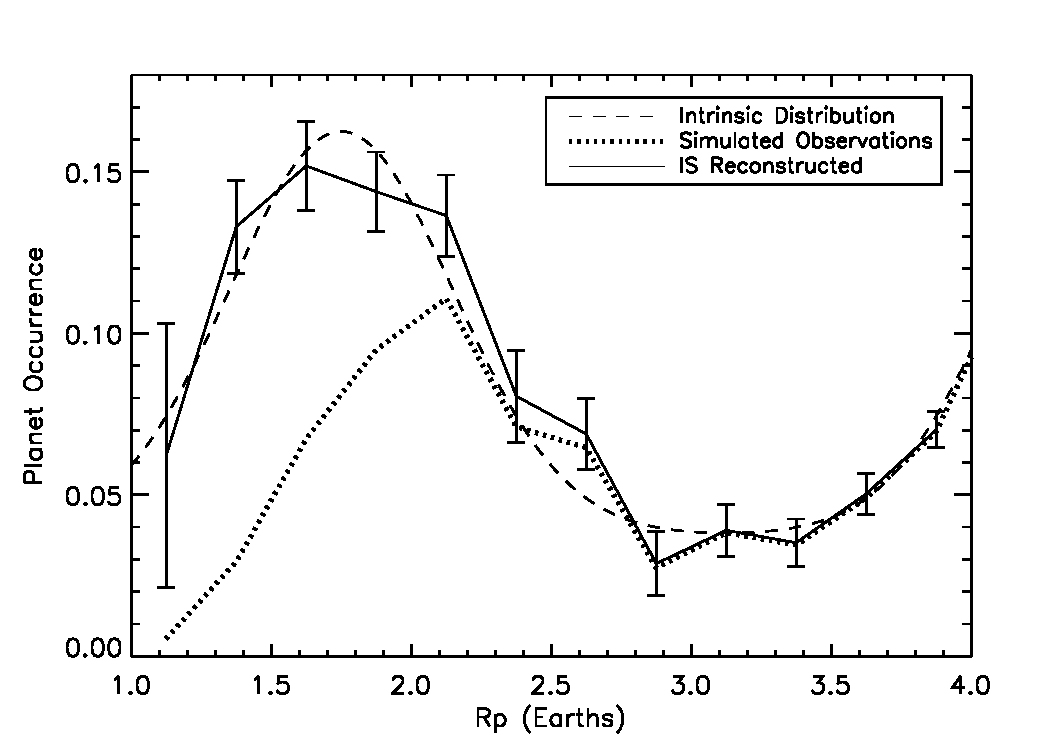
\includegraphics[scale=0.55]{chap2/IStest.pdf}}
\caption{A test case demonstating the recovery of a known, artificial
  radius distribution (dashed line) using the method of iterative
  simulation.  The dotted line represents the simulated observations,
  which consist of 364 detections, and the solid line is the
  reconstructed distribution (here binned for display).  Error
  bars are determined from 25 bootstrapped simulations.}
\label{fig:IS}
\end{figure}

\subsection{Calculation of Occurrence}
\label{sec:calocc}

After obtaining best-fit distributions from our MCMC and IS
analyses, we calculate the rate of planet occurrence as a function
of $P$ and $R_p$. We generate $10^6$ mock star-planet pairs and the corresponding
simulated detections (\S \ref{sec:geneq}). These planets are binned in
a logarithmic grid of $P$ (index $i$) and $R_p$ (index $j$). The
occurrence $f(i,j)$ in the bin $(i,j)$ is then
\begin{equation}
f(i,j) = \frac{K_{ij}}{N_*}\frac{N_{*,S}}{S},
\label{eq:ISocc}
\end{equation}
where $K_{ij}$ is the false positive-corrected \citep[Table
1,][]{Fressin2013} number of KOIs falling into the bin $(i,j)$,
$N_{*}$ (=76,711) is the total number of \kep{} target stars in
the Solar76k sample, $N_{*,S} (=10^6)$ is the total number of
mock pairs, and $S$ is the number of simulated detections.  
The ratio $S/N_{*,S}$, the fraction of mock pairs that should be detected, 
and is the product of the geometric factor $R_*/a$ as well as the detection 
completeness in bin $(i,j)$, hereafter known as $C(i,j)$ (see \S
\ref{sec:completeness}).  We then sum over all bins to obtain the total 
occurrence, $f$.

To demonstrate the importance of accounting for radius errors 
(\S\ref{sec:plerr}) when calculating occurrence, we also conduct 
a separate analysis which excludes radius errors. Observed planets are 
binned as above and we calculate the occurrence of each bin, $f$ according to:
\begin{equation}
f(P_i,R_i) = \frac{1}{N_*}\sum\limits_{k}^{n_p(i,j)}\left(\frac{a_k}{R_{*,k}}\frac{1}{C(i,j)}\right)
\label{eq:occtw}
\end{equation}
Where $C(i,j)$ is the average completeness of the bin (see \S
\ref{sec:completeness}), $n_p(i,j)$ is the number of planets in bin $(i,j)$, 
$N_*$ (=76,711) is the total number of stars in the sample and $a_k/R_{*,k}$ is 
the geometric correction factor for planet $k$. 

%%%%%%%%%%%%%%%%%%%%%%%%%%%%%%%%%%%%%%%%%%%%%%%%%%%%%%%%%%%%%%
\section{The Primordial Population of \kep{} Planets}

\subsection{Completeness}
\label{sec:completeness}

For a transit survey, completeness is the fraction of transiting
planets of a given $P$ and $R_p$ that are actually
detected, i.e. not including the geometric transit probability. 
Accurately capturing the dependence of completeness
on $R_p$ and $P$ is crucial to a robust determination of planet
occurrence.

We emphasize that survey completeness depends not only on
the properties of the planet host stars, but also on the stellar
and noise properties of the entire catalog.  We calculate
the completeness $C(i,j)$ of bin $(i,j)$ by inserting $2\times
10^4$ planets randomly distributed around the Solar76k
sample of stars. The fraction of ``detected'' planets, modulo the
transit probability factor, yields the completeness in this bin.
The results are displayed in Figure~\ref{fig:sil_compl}.

\begin{figure}
\centerline{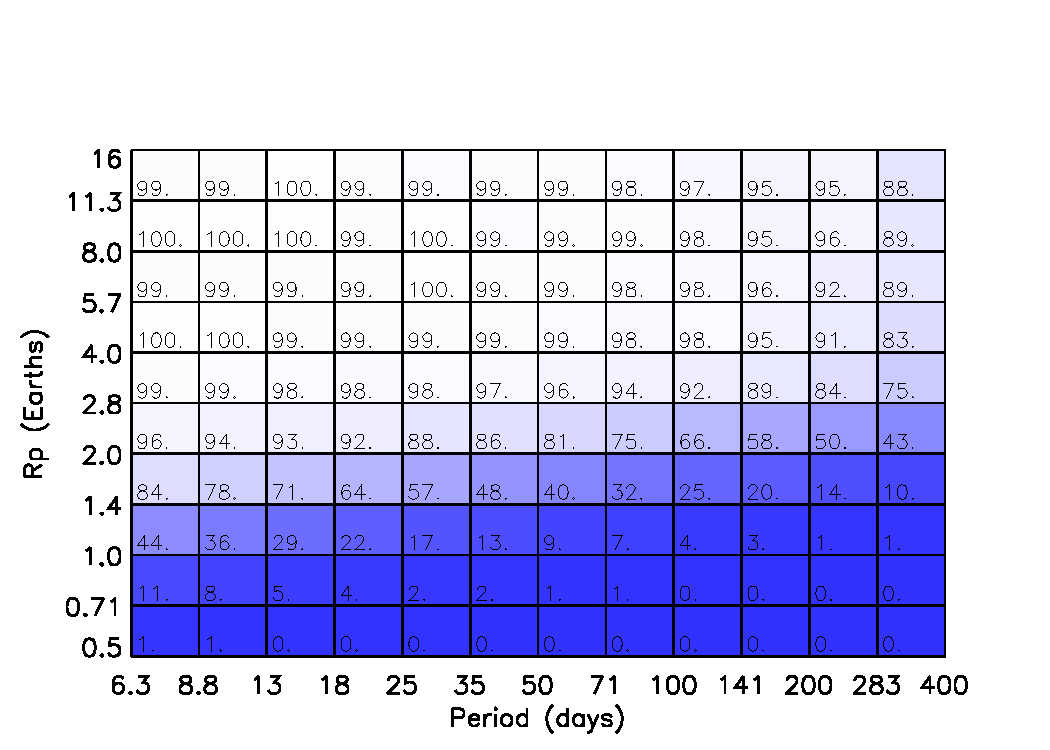
\includegraphics[scale=0.55]{chap2/Silburt_completeness.pdf}}
\caption{Completeness values for \kep{} planet detection around stars 
  in the Solar76k catalog. The numbers within each grid cell indicate 
  the completeness percentage, and each grid has been colour coded from low
  (blue) to high (white) completeness.}
\label{fig:sil_compl}
\end{figure}

Figure~\ref{fig:sil_compl} shows that \kep{} completeness is nearly 100\% 
for planets larger than
Neptune (3.8\rearth{}) and for nearly the full range of periods shown
here. This falls rapidly beyond $P \sim $ 500~d (not shown)
since some systems no longer have the required three
transits during the four-year \kep{} mission. The completeness
drops rapidly with decreasing radius where $R<2$\rearth{}:
Earth-sized planets are readily detected by \kep{} only if they have
orbital periods of a few days, and beyond $P=200$~d, even the
completeness of $2 R_\oplus$ planets falls below 50\%. For these
reasons we restrict our analysis to $P < 200$d.   As true of 
any completeness study, we also note that 
our completeness calculations are based on the SNR criterion as 
stated. For example, if the \kep{} pipeline 
was uniformly missing 25$\%$ of all transiting planets (regardless 
of the SNR), our completeness calculations would not account for these
missing planets.


%Moreover,
%  we find that our completeness estimates diverge from those of PHM13
%  beyond this point (see \S\ref{sec:petcomp}). 

\subsection{Period Distribution}
\label{sec:intperiod}

Our MCMC study yields a best-fit distribution for the 430KOI sample of
$\alpha=-0.04 \pm 0.09$ (see Eq.~\ref{eq:P}), with a reduced 
chi-squared $\chi^2_{\nu}$ of
1.07. Our value of $\alpha$ is consistent with zero (a flat
logarithmic distribution) within errors, confirming previous
determinations \citep[e.g.,][]{Youdin,Howard2012,Petigura2013,Fressin2013}.

Figure~\ref{fig:period} compares this best-fit period distribution
with the observed sample, using the 4 period bins from Section~\ref{sec:mcmc}
as well as an additional 2 bins to include to include planets inward of
$20$~d, i.e., the 1052KOI sample (\S\ref{sec:catalogs}).
Inside of $P = 20$~d, \kep{}
planets deviate from a simple power-law distribution \citep[also
see][]{Youdin,Howard2012}.

\begin{figure}[h]
\centerline{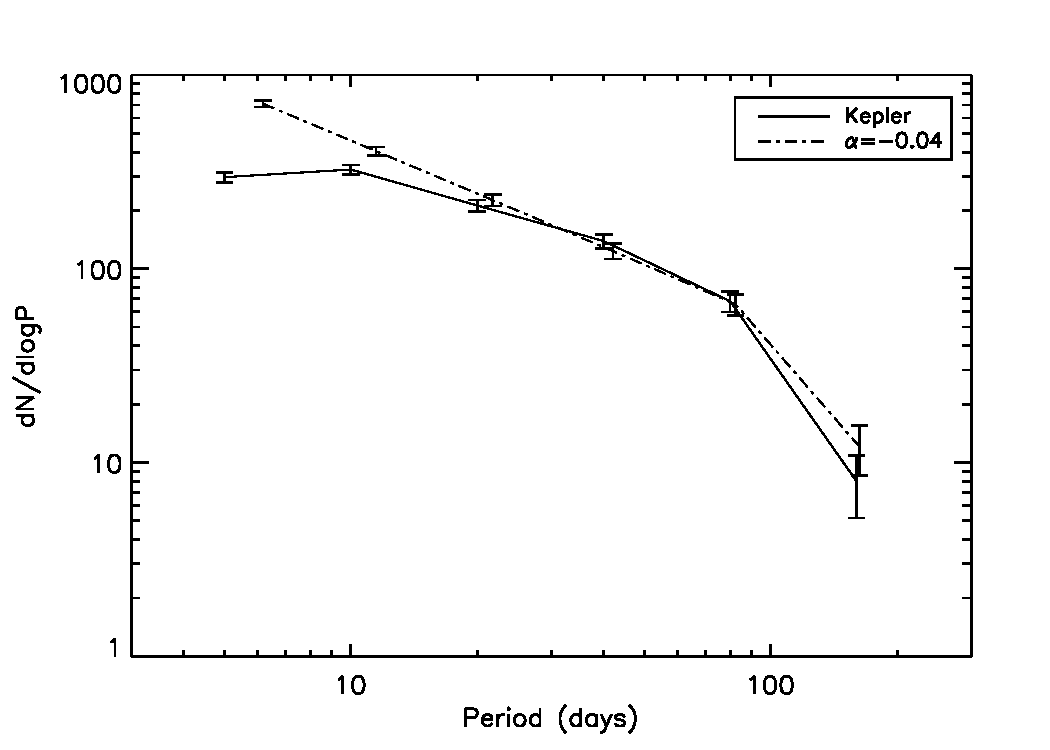
\includegraphics[scale=0.55]{chap2/Silburt_period.pdf}}
\caption{Period distribution of \kep{} small planets. The observed
  distribution (solid line) includes planets inward of $20$~d (i.e. the
  1052KOI sample), while the simulated distribution from the MCMC best
  fit ($\alpha = -0.04$, see Eq.~\ref{eq:P}) is plotted as a
  dashed-dotted curve. This best fit is obtained for planets in the $20 <
  P < 200$~d range, but is extended here to shorter periods to
  demonstrate that the observed population deviates significantly from
  a single power-law shortward of $20$~d. The location of each data point
  corresponds to the lowest period value in the bin, e.g. the first data point is 
  $5<P<10~d$. Slight horizontal offsets have been applied to each curve for clarity.}
\label{fig:period}
\end{figure}

%%%%%%%
\subsection{Radius Distribution}
\label{sec:radiusdist}

Figure~\ref{fig:raddist} displays our best-fit radius distributions
for both the MCMC (solid, black) and IS (dotted, red) techniques,
where we have binned the IS result for ease of comparison.  Both the IS and MCMC
distributions peak at 2--2.8\rearth{} and decrease towards smaller
radii.  We have also plotted two additional distributions in
Figure~\ref{fig:raddist}, a ``No Error'' case (dashed, green)
constructed from Eq.~\ref{eq:occtw} and a ``25$\%$ Larger'' IS case
(dashed-dotted, blue) where it is assumed that both planet and stellar
radii are 25$\%$ larger than their catalog values.

% (note that in Figure~\ref{fig:raddist} the IS is binned only for
% comparison purposes).

%
\begin{figure}
\centerline{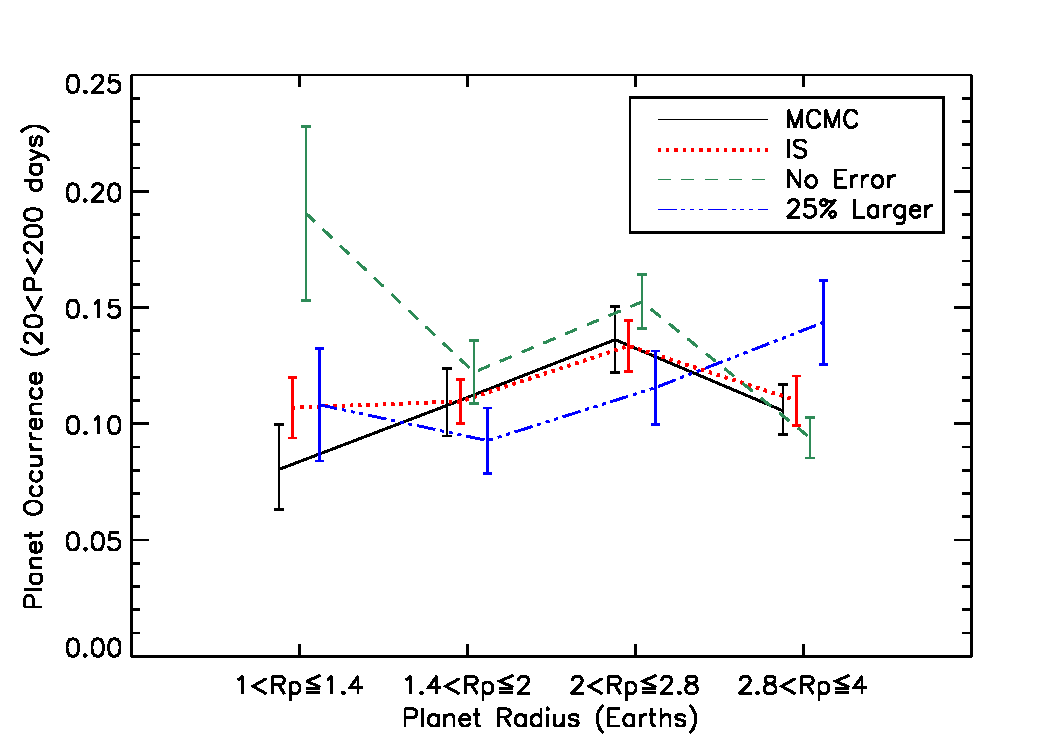
\includegraphics[scale=0.55]{chap2/Silburt_Rdist_all.pdf}}
\caption{Size distribution of planets between 1 and 4\rearth{},
  obtained using the MCMC (solid black line) and the IS (dotted red
  line) techniques. Both show that planet occurrence peaks in the bin
  2--2.8\rearth{}. Earth-sized planets are less common, 
  though the statistical significance of this result is
  still low. If we assume that the currently determined planet radii
  carry no uncertainty, or that all stars (and hence planets) have
  $25\%$ larger radii than their cataloged values,
  we obtain rather different radius distributions. The error bars for
  the ``No Error'' case account for poisson error only, while for the
  IS and 25$\%$ Larger cases, error bars are calculated from 50 bootstrapped
  simulations of the data (see \S \ref{sec:plerr}). The MCMC error bars are 
  calculated in the standard manner. Planet occurrence at
  each logarithmic radius bin is obtained by summing over all period
  bins.  Slight horizontal offsets have been applied to each curve for clarity.}
\label{fig:raddist}
\end{figure}
 
As we discuss in \S \ref{sec:plerr}, errors in the radius of candidate
\kep{} planets, primarily due to uncertainties in stellar radius, are
large and detection bias against small planets means that a planet's
cataloged radius is likely an underestimate. Comparing our IS and MCMC 
results (which include radius errors) with our ``No Error'' case (which 
doesn't include radius errors) we see that the latter exhibits a significant excess of
1--1.4\rearth{} planets. This is as expected. Correcting for radius error in a
Bayesian way (\S \ref{sec:plerr}) tends to promote small planets to
larger size bins, and de-populates the smallest radius bin. However, planet occurrence of
the two largest bins does not increase significantly since the survey 
completeness is substantially higher in these bins compared to the 
1--1.4\rearth{} bin. We conclude that not accounting for this detection bias 
on radius leads to an erroneously high (by a factor of $\sim 2$)
value of occurrence for the 1--1.4\rearth{} bin.

If we assume the extreme scenario that the true radii of all
stars (and therefore their planets) are 25\% larger than the KOI
values (``25\% Larger'' case in Fig. \ref{fig:raddist}), as is shown
to be the case for at least a subset of the \kep{} stars (\S
\ref{sec:sensitivity}), we observe that the 2--2.8\rearth{} peak is now shifted to
2.8--4\rearth{}. However, we do not see a significant change in
the bin 1--1.4\rearth{} because the depopulation of this region 
(due to increased planet radii) is roughly balanced by a decrease
in completeness as the stars have also become larger. See \S
\ref{sec:sensitivity} for a more detailed discussion.

Our treatment for the radius error is far from
perfect. Some genuinely small planets may, under our procedure, be
wrongly inferred to have larger radii. A better treatment will require
improved errors in stellar/planet radius (see, e.g. \S \ref{sec:improvements}).

There is a small and statistically insignificant discrepancy
between the MCMC and IS results at the smallest bin ($1<R_p<1.4$\rearth{}).  
Since the two methods use
identical input catalogs (\S \ref{sec:catalogs}) and detection
algorithms (\S \ref{sec:geneq}), the difference could be due to the
intrinsic binning in the MCMC method. 

We test the effect of 
different bin sizes on our MCMC results 
by varying the bin sizes in both radius and period space. Using the
logarithmic binning scheme to describe the width, $w$, of each bin:
\begin{equation}
w(n) = 10^{Kn}
\label{eq:KMCMC}
\end{equation}
where $n$ is the bin number and $K$ is a constant, we 
investigate the effect of varying $K$ (and thus bin size) on occurrence.  
When varying period bin size, $K_p$, and keeping the radius bin size, $K_r$, 
constant we find no effect on occurrence, even when $K_p$ is varied by a factor 
of 2. However, when $K_p$ is kept constant and $K_r$ is varied, we do find an affect on  
occurrence rates shown in Figure~\ref{fig:bintest} (where our IS result from 
Figure~\ref{fig:raddist} is plotted as a dotted black line). 
As $K$ is increased (larger bins), we see that the occurrence of $2<R_p<2.8$\rearth{} planets 
increases while the occurrence of $2.8<R_p<4$\rearth{} planets decreases, becoming 
significantly different from our IS result for extreme cases. In contrast, there is no statistically 
significant difference in the smallest bin. We find that 
the error bars increase with more extreme bin sizes, indicating that the MCMC algorithm
has a harder time converging. The default bin sizes for the MCMC result in
Fig.~\ref{fig:raddist} are $K_p$=0.301 and $K_r$=0.150515.

\begin{figure}
\centerline{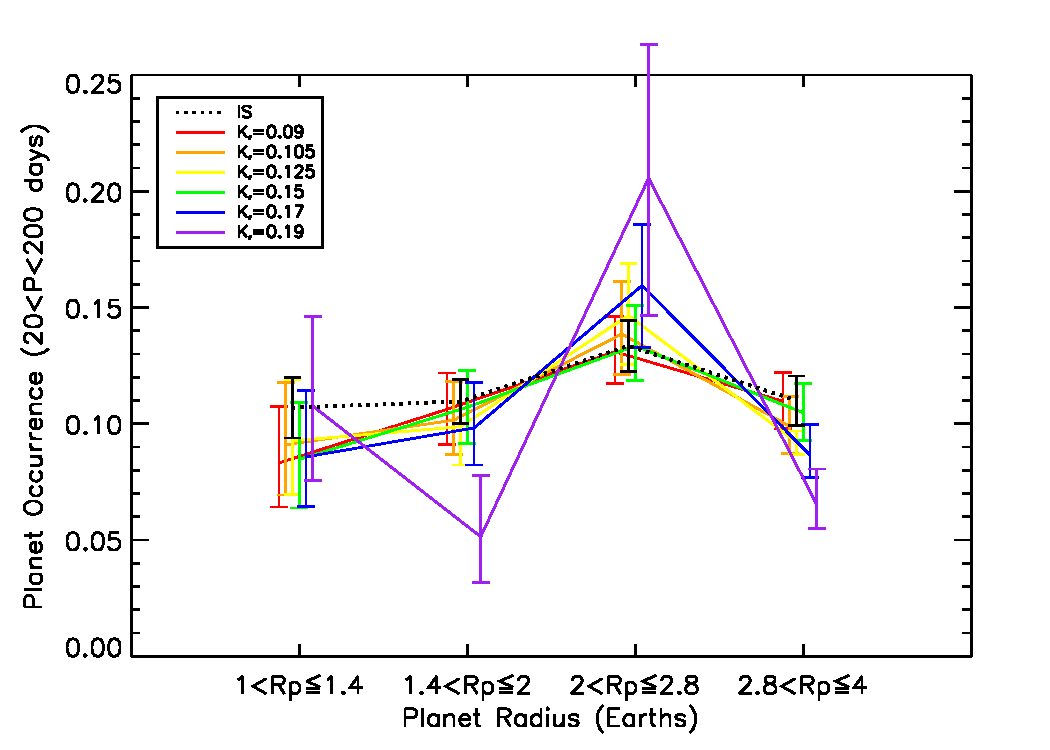
\includegraphics[scale=0.55]{chap2/Silburt_mcmcbin_decRp3.pdf}}
\caption{Investigating the effect of binning on the MCMC results. The IS result from Figure~\ref{fig:raddist} is shown as a dotted, black line, 
while our MCMC results using various bin sizes are the coloured curves. Using
Equation~\ref{eq:KMCMC}, we vary $K_r$ from 0.09 to 0.19, keeping $K_p$ fixed. 
As can be seen, the results can change noticeably depending on
the binning choice. This illustrates the usefulness of the IS method, which does not 
require any binning. To clarify, we do not change the number of free parameters in our
MCMC analysis (i.e. $\kappa_1, \kappa_2, \kappa_3, \alpha$), merely the size of the
bins used to calculate $\chi^2$ values. Horizontal offsets have been added for clarity.}
\label{fig:bintest}
\end{figure}

\begin{figure}
\centerline{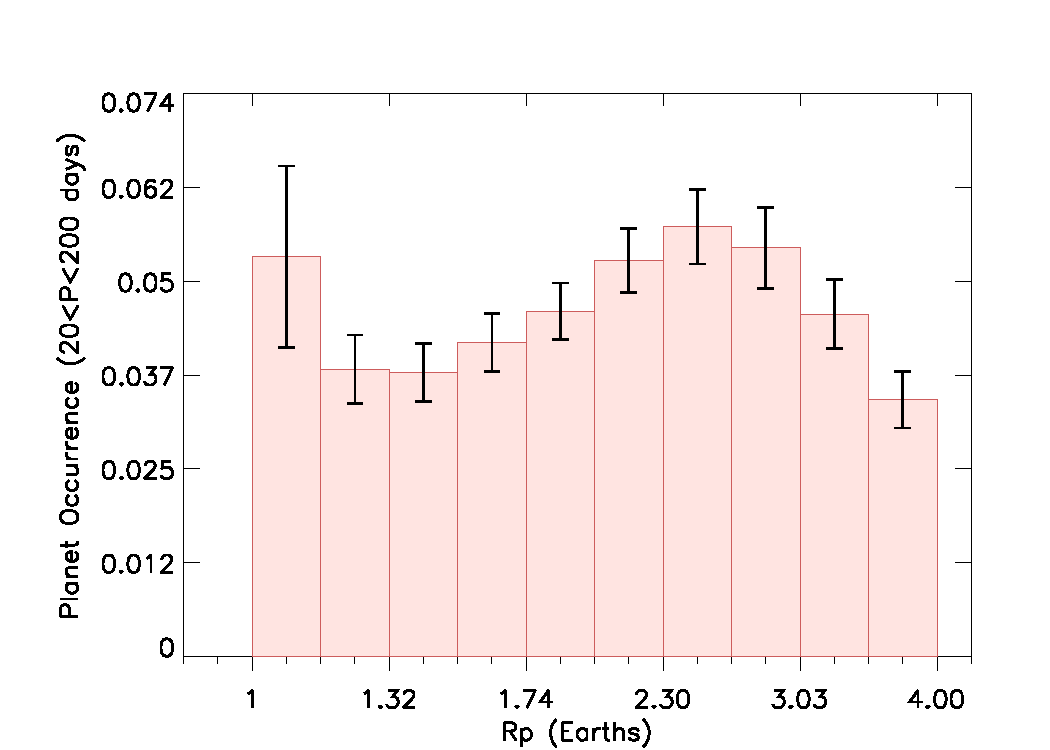
\includegraphics[scale=0.55]{chap2/Silburt_ISnobin.pdf}}
\caption{Our IS distribution displayed for a smaller logarithmic 
 bin size. This finer resolution reveals more information about
 the intrinsic distribution, and specifically we see a potential
 rise in the number of 1--1.15\rearth{} planets. This bin has large 
 error however, and thus more statistics are required to confirm this 
 conclusion.}
\label{fig:isnobin}
\end{figure}

Lastly, we display the IS radius distribution for a smaller
logarithmic bin size in Figure~\ref{fig:isnobin}. As explained in 
\S\ref{sec:IS}, since the IS technique requires no binning, the 
resolution of the result is limited only by the data and its errors. 
This improved resolution can reveal finer detail about the intrinsic 
radius distribution. We observe a slight excess of planets in the now 
smallest bin (1--1.15\rearth{}), over that in larger bins, though improved 
statistics are required to confirm this upward turn.  We
expect that, with its independence on binning, the IS technique will
become central to future analysis.


\subsection{Total Occurrence of Small Planets}
\label{sec:totaloccur}
In Table~\ref{tab:occ} we report our estimates for the total planet
occurrence within $20 < P < 200$~d and $1 < R_P < 4$\rearth{}, for
the four curves in Figure~\ref{fig:raddist}. There is excellent
agreement between the MCMC and the IS results. Even cases with
different assumption about the radius error yield statistically
consistent occurrence rates.

The total occurrence rate we calculate here is defined to be the
average number of planets per star
\citep{Youdin,Fressin2013,Petigura2013}. Such a definition ignores
the complication that many of the \kep{} systems are multiple
systems \citep[e.g.][]{Lissauer2011}. A quantity perhaps more
relevant for studies of planet formation is the occurrence
rate of planetary systems, or the average number of planetary
systems a star has. However, this requires knowledge of the system
architecture, a task not yet attempted.  

Lastly, if we include small planets on orbits interior to $20$~d, the total
occurrence rate is raised to $\sim 66\%$. It will rise by another
$\sim 15\%$ if we include planets larger than $4 R_\oplus$.

\begin{table}[h]
\centering
\caption{Planet Occurrence for $20<P<200$~d, $1<R_p<4$\rearth{}.}
\begin{tabular}{c|c}\hline Technique & Planet Occurrence ($\%$)\\\hline
MCMC                   & $43 \pm 3$ \\
IS                     & $46 \pm 3$ \\
No Error               & $56 \pm 10$ \\
25$\%$ Larger Stars    & $46 \pm 3$ \\
\hline
\end{tabular}
\label{tab:occ}
\end{table}

\subsubsection{Eta-Earth}

We estimate \ee{}, the occurrence of Earth-like planets in the
``habitable zone'' of solar-type stars. By Earth-like, we are
referring to planets between 1--2\rearth{}.  We adopt the inner
and outer boundaries of the habitable zone to be those calculated by
1-D, cloud-free, climate models \citep{Kasting,Kopparapu2013a}.
For a Sun-like star, these boundaries lie at $0.99$ and $1.70$ AU respectively
(or orbital periods of 350 and 810 days); for other stellar spectral
types, the boundaries are as tabulated in \citet{Kopparapu2013a}.

Such a habitable zone, however, lies outside the $200$~d limit of
our study. At these very long periods, the low detection efficiency of
\kep{} engenders inaccuracies in estimating \ee{}. So instead, we have
opted to calculate \ee{} by extrapolation, according to:
\begin{equation}
\eta_{\oplus} = \frac{f}{N_*}\sum\limits_{i=1}^{N_*} h_i
\end{equation}
where $N_*$ (=76,711) is the number of stars in the Solar76k
sample and $h_i$ is the relative occurrence of planets (per star)
within the habitable zone to some reference zone having absolute
occurrence $f$.  We choose this reference zone to be our standard $20 < P <
200$d, $1 < R_p < 4 R_\oplus$ bound, with $f=0.46 \pm 0.03$ (IS
value). We calculate $h_i$ for each star by adopting the IS
radius distribution (Figure~\ref{fig:raddist}) and integrating
the MCMC best-fit power-law (Eq. \ref{eq:P} with $\alpha=-0.04$) over
each star's habitable limits \citep{Kopparapu2013a}.  Finally, we obtain
\begin{equation}
\eta_{\oplus} = 6.4^{+3.4}_{-1.1} \%
\end{equation}
The error is calculated from error propagation of the IS radius
distribution, occurrence of our reference zone, habitable zone limits 
(based on $R_*$, $M_*$, and $T_*$) and $\alpha$.  
This value is consistent within errors with
the analysis done by PHM13 for the same \citet{Kopparapu2013a} limits,
$8.6$\%. The reader is reminded that our calculation of \ee{} is an
extrapolation, and depends crucially on the assumptions made.

\section{Comparison with PHM13}
\label{sec:petcomp}

We now compare PHM13 - an analysis which
is similar to ours in terms of scope but which obtains their results
of the \kep{} data using the TERRA pipeline \citep{Petigura2013}. The TERRA 
pipeline is an analysis tool independent of the \kep{} project pipeline and its
products on which our work relies.  

We first compare our estimates of detection completeness $C$ with that
of PHM13.  For this completeness comparison, we re-compute $C$ using the Best42k
stars from PHM13 and compare these results to the values in Figure S11
from PHM13.  We calculate the fractional difference ($2(T-P)/(T+P)$,
where $T$=This Work and $P$=PHM13) and display as percentages in
Figure~\ref{fig:comp_comp}.  
\begin{figure}[h]
\centerline{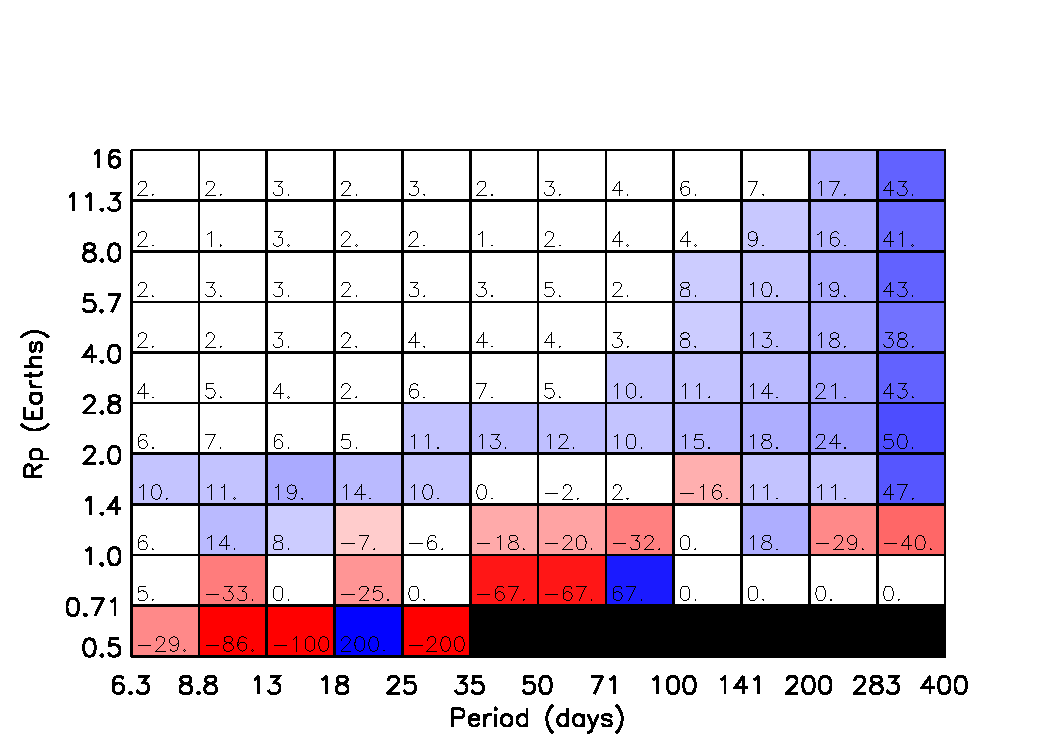
\includegraphics[scale=0.55]{chap2/Petigura_Sil_frac_completeness.pdf}}
\caption{Comparison of completeness values computed with our methods
  to those reported by PHM13 in Figure S11, expressed as a fractional
  difference (i.e. in percentages).  Our values are generated using the ``Best42k'' catalog
  from PHM13 and our detection criteria.  Bins where both our
  completeness and those of PHM13 are zero have been blacked out.}
\label{fig:comp_comp}
\end{figure}
With the exception of a single cell all
values of $C$ in the range $P$ = 20--200~d, and $R_p$= 1--4\rearth{}
are within 20\% of PHM13 values.  This shows that even a comparatively
simple description of \kep{} planet detection can account for most of
the statistics.  The single exception is for the 1--1.4\rearth{} and
71--100~d bin where our estimate of $C$ is 32\% lower than that of
PHM13.  This bin includes the 90~d roll-period of \kep{}.  Large
systematics appear in raw \kep{} lightcurves at this period because
the stars change positions on the detector array.  It might be
expected that the planets with $P$ near 90~d would be more
difficult to detect than our naive criteria and that actual
completeness would be lower.  If the PHM13 values are more realistic,
then the opposite appears to be the case.  Elsewhere in $P$-$R_p$
space our completeness values are slightly and systematically higher
than those of PHM13, and the discrepancy increases with increasing $P$
and decreasing $R_p$.  This is to be expected because PHM13 determine
detection efficiency using actual lightcurves rather than
representations of noise a la CDPP values.  At $P>200$~d our values of
$C$ become significantly higher than PHM13 for nearly all values of
$R_p$.  This discrepancy motivates our restriction to $P < 200$~d.
One possible explanation for this difference is that detection of
signals by phase-folding in the \kep{} detection pipeline becomes
inefficient at long periods.

We note that PHM13 calculates completeness 
based on a finite number ($4 \times 10^4$) of systems of which very few detections 
are in the Earth-sized bins, leading to large counting (Poisson) error in completeness 
values.  Since we use a different approach, simulating large numbers ($2 \times 10^6$ total, 
$2 \times 10^4$ per bin) of test planets and giving high drawing probability 
to Earth-sized planets, we are able to simulate a much larger number of detections 
for each bin and thus have a more precise (although not necessarily more accurate) 
value of completeness.

\begin{figure}
\centerline{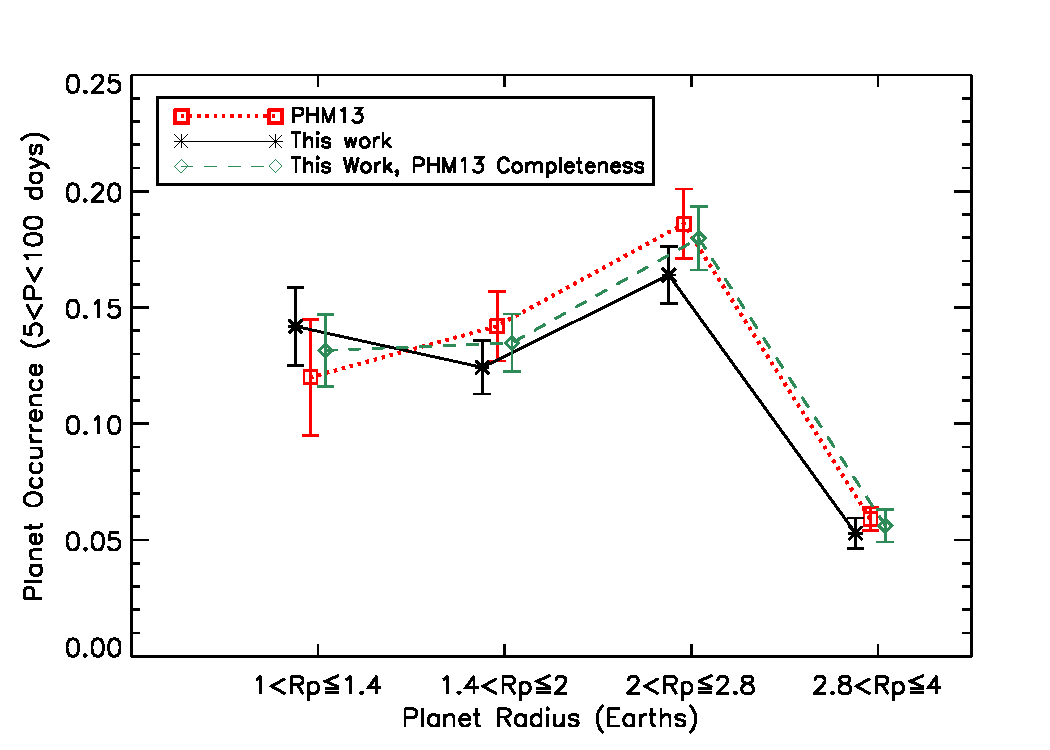
\includegraphics[scale=0.55]{chap2/PHM13_mastercomp.pdf}}
\caption{A summary of our comparison to PHM13, plotted in percentages 
  along the y-axis. All curves are constructed using the ``603PHM'' 
  dataset and ``Best42k'' sample. The results
  of PHM13 are plotted as the dotted curve in red with
  squares, ``This work'' uses our own completeness values, and is the black
  solid curve in black with stars, ``This work, PHM13 Completeness'' uses PHM13's Figure
  S11 completeness values and is the green
  dashed curve with diamonds. Slight horizontal offsets have
  been applied to each curve for clarity.}
\label{fig:mastercomp} 
\end{figure}

We next compute the impact of these differences in completeness on
occurrence over $P$=5--100~d, shown in Figure~\ref{fig:mastercomp}. We first 
calculated occurrence using the ``603PHM'' dataset (\S\ref{sec:catalogs}),
Eqn.~\ref{eq:occtw} along with our own detection criteria (\S \ref{sec:geneq}) and completeness
values (calculated from the Best42k sample), shown as the solid black curve in
Figure~\ref{fig:mastercomp}. We then re-calculated planet occurrence
using the 603PHM dataset, Eqn.~\ref{eq:occtw} along with our own detection criteria
but substituting in the completeness values from Figure S11 of PHM13 for
ours, shown as the dashed green line in Fig.~\ref{fig:mastercomp}. Lastly,
the direct results of PHM13 are shown as a dotted, red line. 
The differences between all curves in
Figure~\ref{fig:mastercomp} are small and, within errors, agree with
each other. The residual differences in completeness
seen in Fig.~\ref{fig:comp_comp} do not appear to play a significant role in the
comparative occurrence of our work and that of PHM13 but could be
responsible for some of the minor (and statistically insignificant)
differences that we find. {\it We conclude that simple detection
criteria and noise model can be used in planet occurrence studies to achieve
accurate and precise results}.

Comparing PHM13's intrinsic radius distribution 
(red curve in Figure~\ref{fig:mastercomp}) to our own (black curve in Figure~\ref{fig:raddist}), 
we notice a difference in the occurrence of large ($2<R_p<4$) planets.
Specifically, PHM13 calculated an occurrence of $18.5 \pm 1.5\%$ and $6 \pm 0.5\%$ 
for $2<R_p<2.8$ and $2.8<R_p<4$ planets, respectively, while we find
an occurrence of $13.0 \pm 1.1\%$ and $10.5 \pm 1.0\%$ for the same bins. This results in a statistical 
difference of about $2\%$ and $3\%$ between works for the $2<R_p<2.8$ 
and $2.8<R_p<4$ bins, respectively. 
We see a few possible reasons for this. Table~\ref{tab:comp} displays the major differences 
in raw samples between our work and PHM13, displaying the raw occurrence of large 
($2<R_p<4$\rearth{})
planets for their nominal period ranges, $P>20$~d and $P<20$~d. The bottom two rows of
``This Work'' are empty in Table~\ref{tab:comp} since all of the planets in our sample are $P>20$, 
and thus all the relevant information is present in the first row.  
\begin{table}[h]
\centering
\caption{Differences in raw counts between our work and PHM13}
\begin{tabular}{|c|cc|}\hline Range & This Work & PHM13 \\\hline 
Nominal $P$ range: & & \\
$1<R_p<4$\rearth{} (Total) & 394 & 495 \\
$2<R_p<2.8$\rearth{} & 166 ($42 \%$) & 191 ($39 \%$) \\
$2.8<R_p<4$\rearth{} & 120 ($30 \%$) & 87 ($18 \%$) \\\hline
$P>20$~d: & & \\
$1<R_p<4$\rearth{} (Total) & -- & 201 \\
$2<R_p<2.8$\rearth{} & -- & 89 ($44 \%$) \\
$2.8<R_p<4$\rearth{} & -- & 45 ($22 \%$) \\\hline
$P<20$~d: & & \\
$1<R_p<4$\rearth{} (Total) & -- & 294 \\
$2<R_p<2.8$\rearth{} & -- & 102 (35$\%$)\\
$2.8<R_p<4$\rearth{} & -- & 42 (14$\%$) \\\hline
\end{tabular}
\label{tab:comp}
\end{table}

To summarize Table~\ref{tab:comp}, of the 394
KOIs in our raw planet sample between $1<R_p<4$, 166 ($42 \%$) and 120 ($30 \%$) 
are between $2<R_p<2.8$\rearth{} and $2.8<R_p<4$\rearth{}, respectively, 
while for PHM13, of the 495 KOIs between $1<R_p<4$\rearth{}
only 191 ($39 \%$) only 87 ($18 \%$) fall into the same limits, respectively. 
This is a significantly lower fraction, and it appears the two samples 
are markedly different. There are only a couple options available to explain this difference -- 
either a disproportionate number of large 
($2<R_p<4$\rearth{}) planets in our sample are false positives, 
or the two datasets are not subsamples from the same population. 

If the two samples are from different populations, this difference could be due to the
photoevaporation \citep{Owen2013} of PHM13's close-in planets, 
which acts to convert large ($2<R_p<4$\rearth{})
planets into smaller ones. Analyzing he PHM13 dataset
adds support to this theory, since as we move from $P>20$~d to $P<20$~d planets, 
raw occurrence drops proportionally (i.e. relative to the entire $1<R_p<4$\rearth{} sample) by 
$(44 \% - 35 \%)/ 44 \% \sim 20 \%$ and $(22 \% - 14 \%)/ 22 \% \sim 40 \%$ for 
$2<R_p<2.8$\rearth{} and $2.8<R_p<4$\rearth{}  
planets, respectively.

%\citet{Mulders2014} recently 
%found that planet occurrence rates are dependent upon stellar sample, and as
%can be seen in Figure~\ref{fig:kiccomp} our stellar sample is significantly different from
%PHM13's, with our sample containing proportionally more $0.8<R_s<1.2$ stars. 
%However, it should be noted that \citet{Mulders2014} only considers 
%$P<50$d planets and does not predict a significant change for $2.8<R_p<4$\rearth{} planets. 

%\begin{figure}[h]
%\centerline{\includegraphics[scale=0.55]{starcomp_kic.pdf}}
%\caption{ A comparison of our Solar76k sample (grey) to the Best42k sample of PHM13 (black). 
%	As can be seen, the stellar samples are significantly different. }
%\label{fig:kiccomp}
%\end{figure}

In explaining the difference between the occurrence of large planets between this work and PHM13, 
one must also consider the improved treatment of
radius errors and updated \citet{Huber2014} stellar parameters used in this work. 
Both tend to increase planet size, pushing smaller planets into larger bins.
Comparing the ``No error'' case to the ``IS'' case in Fig.~\ref{fig:raddist}, we can see that
the former effect increases the occurrence of $2<R_p<2.8$\rearth{} and $2.8<R_p<4$\rearth{} 
planets by about 2$\%$ and 1.5$\%$, respectively. Thus, it appears that 
the discrepancy of our results with the PHM13 in the $2<R_p<2.8$\rearth{} bin can
be explained by our incorporation of radius errors. However this does not 
account for the total discrepancy in the $2.8<R_p<4$\rearth{} bin, leaving about $1.5\%$ of
discrepancy between our work and PHM13. 

Finally, PHM13 reported an occurrence of $37 \pm 3.4\%$ for planets with 
$25<P<200$~d and $1<R_p<4$\rearth{}. Including planets from 
$20 < P < 25$~d raises this value to $42 \pm 3.6\%$.  
So the overall occurrence rates are consistent among
studies that are based on different detection criteria and different
model assumptions. 

%%%%%%%

\section{Discussion}
\label{sec:discussion}

\subsection{Sensitivities and Systematics}
\label{sec:sensitivity}

To investigate sensitivities to some of the assumptions and parameters
in our analysis, we repeat our IS simulations varying $\sigma_e$ and $\alpha$. First,
we varied the Rayleigh distribution of orbital eccentricities between 0.1
and 0.3, and second varied the value of $\alpha$ between -0.15 and 0.15.  
In all cases we found no significant difference in the radius distributions. We also
investigate our separability assumption (Eqn.~\ref{eq:assumption}) by
splitting our 430KOI dataset into two equal sized subsets corresponding to $20<P<50$ and
$50<P<200$~d planets, and performing an MCMC analysis on each. 
The resulting distributions are consistent with each other as well as with our
main IS and MCMC results, indicating that there is no significant
correlation between planet radius and period in our sample, and
that Eqn.~\ref{eq:assumption} is a reasonable assumption.

In this analysis, we address the fact that many \kep{} planets
have large errors in radius, driven primarily
by uncertainties in the radii of their host stars.
But we have not addressed the issue of systematic errors
in stellar radii.  For example,
stellar effective temperatures based on photometry from KIC
\citep{Brown2011} are systematically $\sim$200~K hotter than more
reliable estimates based on the infrared flux method
\citep{Pinsonneault2012} or spectroscopy \citep{Gaidos2013}.  The
combination of uncertainties in stellar parameters and Malmquist bias
in the magnitude-limited \kep{} target catalog means that the
sample is biased towards the most luminous, hottest, and largest stars
\citep{GaidosMann2013}.  There is increasing evidence that many \kep{}
target stars, including planet hosts, are subgiants \citep[e.g.,
][]{Verner2011,Everett2013,Bastien2014}.  For fixed values of
$R_p/R_*$, systematically larger stellar radii means the planets
are also systematically larger and that the geometric transit
probability is higher than presumed (transit probability depends
inversely on stellar density and hotter, more evolved stars are less
dense).  The detection completeness of small planets is also smaller
than presumed and thus, for fixed number of detections, the occurrence
is higher.

We have explored the possible impact of these effects by assuming
that all stellar radii in our Solar76k catalog, as well as all
the planet radii in the corresponding 450KOI catalog, are 25\% larger
than their nominal values (dashed-dotted blue curve, Fig.\ref{fig:raddist}). 
The distribution differs markedly from our IS and MCMC distributions. 
The peak in the distribution at 2--2.8\rearth{} has shifted towards
larger radii.  Surprisingly, the occurrence of planets with $R_p$ =
1--1.4\rearth{} has not changed.  This is understood. As stellar
radii increase, completeness of small planets decrease leading to an
increase in planet occurrence. However, the number of 1--1.4\rearth{}
planets in our sample also decreases (from 25 to 8 after a 25$\%$
radius increase), reducing the raw planet
occurrence in this radius bin. It appears that these two competing
effects roughly cancel, resulting in no significant change in planet
occurrence of the smallest radius bin. 

We now comment on our treatment of false positives in this analysis. 
Our work makes use of the \citet{Fressin2013} false positive rates based 
on the Q1--Q6 \kep{} data, while other works (e.g. PHM13) use custom 
methods to detect false positives. 
However since we use the latest disposition of the \kep{} catalog in this analysis,
the occurrence of false positives in our Solar76k sample could be significantly
different. We calculate the ratio of false positives (``FP'') vetted by the
\kep{} science team to planet candidates (``CAN'') for the Q1--12, Q1--16 and
cumulative \kep{} catalogs according 
to FP/(FP+CAN). In addition, we organize these false positive ratios by radius, 
using the same radius bins as our analysis. These false positive ratios are shown 
in Table~\ref{tab:fp}, as well as the \citet{Fressin2013} values for reference. 
It should be noted that the fraction of planets yet to be 
dispositioned (calculated according to DISP/(DISP+CAND+FP), where DISP is the 
number of planets yet to be dispositioned) in the Q1--12 and Q1--16 datasets are quite high 
(over 50 $\%$), and may reflect the significant difference between their false positive rates 
and the cumulative KOI dataset rates. 

\begin{table}[h]
\centering
\caption{False positive ratios, calculated according to FP/(FP+CAND)}
\begin{tabular}{c|c}\hline Dataset  & FP$\rightarrow$[1-1.4, 1.4-2, 2-2.8, 2.8-4]\rearth{} \\\hline
\citet{Fressin2013} & 0.088, 0.088, 0.067, 0.067 \\
Q1--12             & 0.37, 0.39, 0.27, 0.24 \\
Q1--16             & 0.28, 0.31, 0.36, 0.53  \\
Cumulative      & 0.22, 0.24, 0.16, 0.19 \\
\hline
\end{tabular}
\label{tab:fp}
\end{table}

%\begin{figure}[h]
%\centerline{\includegraphics[scale=0.55]{fp_v_time_radius.pdf}}
%\caption{ {\y False positive rates as a function of \kep{} catalog, calculated by
%FP/(CAND + FP), where ``FP'' is the number of false positives and ``CAND'' is
%the number of planet candidates. Arranged
%as a function of radius, the red, orange, blue and purple curves correspond 
%to radius bins of $1 < Rp < 1.4$\rearth{}, $1.4 < Rp < 2$\rearth{}, $2 < Rp < 2.8$\rearth{},
%$2.8 < Rp < 4$\rearth{}, respectively. In addition, we also plot the ratio of 
%planets not yet dispositioned by the \kep{} science team, ``DISP'', as 
%DISP/(FP + CAND + DISP). Lastly, the false positives in the Q1--Q6 catalog 
%were never assigned planet radii, and thus cannot be sorted as a function 
%of radius.}}
%\label{fig:fp}
%\end{figure}

We use the false positive fractions in table~\ref{tab:fp} to estimate the uncertainty
of using \citet{Fressin2013} false positive rates in our analysis. 
For Q1--12, Q1--16 and the cumulative list, 
we carry out separate MCMC analyses substituting in the false positive rates from 
Table~\ref{tab:fp}.  Only the cumulative list remains consistent with our main IS and MCMC
results, with overall occurrence rates of the Q1--12, Q1--16 and cumulative datasets
being $0.30 \pm 3\%$, $0.32 \pm 3\%$ and $0.38 \pm 3\%$, respectively, i.e. much lower
occurrence values. 
Taking the standard deviation of each radius bin for our main IS result (Fig.~\ref{fig:raddist})
plus these three new analyses using Q1--12, Q1--16 and cumulative false positive rates, 
we estimate the uncertainty in our false 
positive rates on the occurrence of planets for $1<R_p<1.4$, $1.4<R_p<2$, $2<R_p<2.8$, and
$2.8<R_p<4$\rearth{} to be 2.1$\%$, 1.6$\%$, 1.8$\%$ and 2.4$\%$, respectively.

%\begin{figure}[h]
%\centerline{\includegraphics[scale=0.55]{Silburt_mcmcbin_fp.pdf}}
%\caption{ {\y We estimate the uncertainty of using \citet{Fressin2013} false
%	positive rates in our analysis, which was originally tailored for the 
%	Q1-6 dataset. In this figure we measure the effect of substituting in the false positive 
%	rates from Figure~\ref{fig:fp} on occurrence. The red, orange and yellow curves
%	correspond to the Q1--12, Q1--16 and cumulative list false positive rates, with our main 
%	IS result shown as a dotted black line for comparison. }}
%\label{fig:mcmcbin_fp}
%\end{figure}

\subsection{Astrophysical and Astrobiological Implications}
The period distribution of \kep{} small planets contains two distinct
parts. The first is a rise from  $\sim$ 5--10~d 
\citep[e.g.][]{Youdin,Howard2012}, the second is a
logarithmically flat distribution extending from $\sim 10$~d out to
at least 200~d \citep[Fig. \ref{fig:period}
here,][]{Petigura2013,Fressin2013}. The origin of both features are
unclear. But we speculate on one origin for the logarithmically flat feature.
Imagine a set of planetary systems comprised of
closely-packed, equal-mass planets. Dynamical stability requires that
neighbouring planets be spaced apart by more than a few Hill radii
\citep{Chambers,Smith2009}. Since the Hill radius scales linearly
with orbital semi-major axis, this means the separation between
neighbouring planets grows linearly with their orbital
span. This would then translate into a period
distribution that is flat in logarithmic period. In other words, it is
possible that most or all of our planets are actually in multiple
systems, and that the flat feature is a result of the stability
requirement. Although \citet{Fang12} have quoted that $75 - 80 \%$
of planetary systems have one or two planets with orbital periods less than 
200~d (suggesting that most systems are not close to the Hill stability limit), this
result is based on the occurrence of {\it observed} systems. Most Earth-sized
planets (or smaller) around Sun-like stars are undetectable by \kep{}, and
it is possible that the multiplicity of such systems are much higher than
we currently believe due to these unseen planets.

Alternatively, the flat feature can arise from the primordial mass
distribution in the disk. Assuming that all planets have comparable
masses, are in multiple systems, and are
formed where they are found today, a logarithmically flat
spacing would suggest that the disk surface density $\Sigma$ scales
with the orbital separation $a$ as,
\begin{equation}
\Sigma \propto a^{-2}\, .
\end{equation}
This is not vastly different from the theoretical MMSN profile:
$\Sigma \propto a^{-3/2}$ \citep{Hayashi1981,Weidenschilling1977}, a
useful benchmark to study proto-planetary disks.

The radius distribution is equally intriguing. The radius of a Earth- to Neptune-sized
planet mostly reflects the expanse of its hydrogen envelope \citep{Wolfgang2014}.  By
focusing on planets outward of $20$~d, we discard candidates that
may have had their atmospheres eroded by stellar irradiation \citet{Owen2013}. The
distribution shown in Fig.\ref{fig:raddist} is therefore likely
``primordial''. Compared to planets inward of $10$~d that have radii
$\leq 1.5 R_\oplus$, this ``primordial'' population appears to prefer a 
size of $\sim 2.5R_\oplus$. Such a size corresponds to a fractional mass in the
hydrogen envelope of $\sim 1\%$ \citep[assuming a rocky core roughly 
in the $10M_{\oplus}$ range, see, e.g.][]{WuLithwick}. What
is the reason behind this preferrence for $1\%$? A planet embedded in
a proto-planetary disk can accrete a hydro-static
atmosphere. \citet{Rafikov} calculated that this atmosphere has a mass
of a few $M_\oplus$ for a $10 M_\oplus$ planet at $0.1$ AU in a MMSN
disk. This lies much above the $1\%$ value but it depends on disk
parameters and its evolution history.  In future works, the observed
radius distribution should be used to decipher formation history.

Moreover, the gradual decline toward smaller
sizes in logarithmic space has implication for the formation of
bare-core planets, the norm in the inner Solar
system. Our terrestrial planets are thought to have formed in a
gas-free environment by conglomeration of solid materials. The
relative shortage of bare-core planets may suggest that the 
observed \kep{} planets may have followed different formation path 
than that of the terrestrial planets.

Lastly, we turn to the issue of \ee{}. We calculate \ee{} more out of
respect for tradition than with any conviction that there is
additional accuracy to be assigned to our calculation.  The limits of
the habitable zone depend on important assumptions regarding the
climate state of Earth-like planets \citep{Kopparapu2013a}, mass
\citep{Kopparapu2014}, and the composition of the atmosphere
\citep{Pierrehumbert2011}.  Nevertheless, the search for life
elsewhere can take heart in the fact that multiple investigations
point to an occurrence of Earth-size planets in habitable zones of
$\mathcal{O}(0.1)$ or more.  Indeed, studies of M dwarfs suggest that
\ee{} $\sim 0.5$ \citep{Bonfils2013,Kopparapu2013b,Gaidos2013}.  M
dwarfs comprise about 70\% of all stars and hence weigh heavily in the
census for Earth-like planets.

\subsection{Improvements in Occurrence will Happen}
\label{sec:improvements}
The errors associated with most \kep{} planets are dominated by
the uncertainty in the parameters of their host stars. Thus, in 
order to improve planet occurrence calculations for the future we 
must first understand \kep{} stars better. 
The {\it Gaia} (Global Astrometric Interferometer for Astrophysics)
mission, launched in December 2013, will measure the parallaxes of 1
billion stars in the local group with accuracies approaching 10
$\mu$as, as well as obtain multi-band photometry measurements
\citep{deBruijne2012}. \citet{Liu2012} estimate that for stars in the
KIC, {\it Gaia} will be able to estimate $T_{\rm eff}$ to 1\%, $\log
g$ to within 0.1-0.2 dex, and [Fe/H] to within 0.1-0.2 dex.  The
combinations of these data should dramatically improve our knowledge
of the properties of \kep{} target stars and hence reconstructions of
the \kep{} planet population.

Other advances include improved maps of interstellar reddening in the
\kep{} field based on the colors of oscillating red giants with
established properties, as well as WISE infrared photometry
\citep{Huber2014}.  The advent of multiplexed, multi-object
spectrographs capable of simultaneously measuring thousands of stars
\citep{Hill2010} should, combined with {\it Gaia} parallaxes, allow
stellar parameter estimation with unprecedented
scale and precision. In addition, measurement of photometric noise due
to stellar granulation (``flicker'') is a promising technique for
estimating the $\log g$ and hence radius of bright \kep{} stars to
within 0.1-0.2 dex \citep{Bastien2014}, although its calibration
and applicability to fainter \kep{} stars -- the majority of targets,
with lower photometric precision -- remains to be seen.

\section{Conclusions}
In this work we have developed a population simulator to
extract the underlying period and radius distributions of Earth- to Neptune-sized
planets detected by \kep{}. We focus on a ``primordial'' population of
planets outside $20$~d to exclude the impact of, e.g. photoevaporation.
We find that the adoption of a simple model of photometric noise and
transit signal detection allow us to accurately estimate the 
survey completeness of \kep{}.  We have accounted
for radius errors in our analysis, and have found that doing so is
important for reconstructing the intrinsic radius disitribution. We
apply the iterative simulation technique to reconstruct the planet distribution
with radius. This does not require binning and allows radius errors to be
readily accounted for. Lastly, we are the first to use
the updated Huber et al. 2014 parameters along with all 16 quarters of
\kep{} data, representing the most up to date analysis. The main
results are as follows: 
\begin{enumerate}

\item The distribution of planets with $20 < P < 200$ days is roughly uniform with
logarithmic period (power-law index $\alpha = -0.04 \pm 0.09$).

\item The (likely primordial) radius distribution for \kep{} planets
  with $20<P<200$d peaks in the radius bin 2--2.8\rearth{}. 
    
\item The overall occurrence of planets within $20<P<200$~d and
  $1<R_p<4$$R_\oplus$ is $46\% \pm 3\%$. This represents the average
  number of planets per solar-type star in the \kep{} field.

\item Extrapolating our radius and period distributions out to the
  habitable
  zone for solar-type stars, we find $\eta_{\oplus}=6.4^{+3.4}_{-1.1}\%$.\\

\item While our results confirm those from earlier studies, 
 there is a discrepancy in the occurrence of planets for $2.8<R_p<4$\rearth{} planets  
  between our work ($10.5 \pm 1.0\%$) and PHM13 ($6.0 \pm 0.5 \%$). Our incorporation of 
  radius errors and updated \citet{Huber2014} stellar parameters account for about half of this 
  discrepancy, while the difference in raw samples account for the remainder. 
  PHM13 includes $P<20$~d planets into their analysis which likely contains 
  photoevaporated planets (see Table~\ref{tab:comp}), decreasing the overall occurrence
  in the $2.8<R_p<4$\rearth{} bin. 
  %If the \citet{Fressin2013} false positive rates are incorrect for our analysis, and are instead much higher (see Table~\ref{tab:fp}), this would make our results even more discrepant with PHM13. 
  Although inconclusive at this time, there is a good chance
  that the increase in the occurrence of $2.8<R_p<4$\rearth{} planets in our analysis 
  is due to the exclusion of planets altered by proximity to their host stars. 
  
 \item In a detailed comparison with PHM13 we find that using CDPP
 values can effectively reproduce the detection completeness found by 
 the more sophisticated analysis of PHM13.

\item Large radius errors are present in the \kep{} data, and failing
  to account for these properly can lead to a different radius
  distribution. Specifically, this tends to result in a large excess
  of earth-sized planets. Increasing the size of \kep{} stars by $25 \%$
  increases the frequency of large planets while keeping the occurrence
  of small planets roughly constant. Many stellar radii in the \kep{}
  catalog are suspected to be underestimated, and GAIA will improve
  these stellar radius errors and resolve this issue.
  
\end{enumerate}

\chapter[Tides Alone Cannot Explain Kepler Planets Close to 2:1 MMR]{Tides Alone Cannot Explain Kepler Planets Close to 2:1 MMR}
\label{chap:Tides}

\section{Chapter Overview}

A number of \kep planet pairs lie just wide of first-order mean motion resonances (MMRs).
Tides have been frequently proposed to explain these pileups, but it is still an ongoing discussion.  
We contribute to this discussion by calculating an optimistic theoretical estimate on the minimum initial eccentricity required by \kep planets to explain the current observed spacing, and compliment these calculations with N-body simulations.
In particular, we investigate 27 \kep systems having planets within $6\%$ of the 2:1 MMR, and find that the initial eccentricities required to explain the observed spacings are unreasonable from simple dynamical arguments.
Furthermore, our numerical simulations reveal \textit{resonant tugging}, an effect which conspires against the migration of resonant planets away from the 2:1 MMR, requiring even higher initial eccentricities in order to explain the current \kep distribution. 
Overall, we find that tides alone cannot explain planets close to 2:1 MMR, and additional mechanisms are required to explain these systems. 

\section{Introduction}
\label{sec:introduction}
The NASA \kep{} mission has been immensely successful for detecting planets outside of our solar system.
To date, it has discovered over 4,500 exoplanet candidates along with 466 multi-planet systems \citep{Akeson2013,Rowe2014}. 
A number of these systems are just wide of a mean motion resonance (MMR), which occurs when the period of one planet is an integer ratio of another. 
In particular, statistical excesses in the period distribution of \kep{} planets have been detected just wide of the 3:2 and 2:1 MMR \citep[][]{Lissauer2011,Fabrycky2014,Steffen2015}.
It is believed that in the past these planetary systems migrated into resonance via convergent migration \citep{Lee2002}, and a number of dissipative mechanisms have been proposed to slowly bring these planets out of MMR.
The most popular dissipative mechanisms to explain the observed near-resonant systems are tidal \citep{LithwickWu2012, Batygin2013, Delisle2014},  protoplanetary \citep{Rein2012b, Baruteau2013, Goldreich2014}, and planetesimal \citep{Moore2013, Chatterjee2015}. 

In this work we focus exclusively on tidal dissipation, for which there is no clear consensus on whether this mechanism alone can successfully explain the excess of near-resonant pairs near first order MMRs. 
Several authors \citep{LithwickWu2012,Batygin2013} have argued for \citep{Delisle2014} tidal dissipation, whereas others \citep{Lee2013} have argued against it. 
In particular, \citet{LithwickWu2012} first introduced the mechanism of \textit{resonant repulsion}, and showed that in the limit of low eccentricities for near-resonant planets, the space between planets grows as~$t^{1/3}$.
\citet{Batygin2013} confirmed this result.
\citet{Lee2013} then used this relationship to show that most near-resonant planet pairs cannot be explained via this mechanism, the few exceptions being small rocky planets for which tidal dissipation is particularly effective.
\citet{Delisle2014} then suggested a high eccentricity mechanism by which planets may still be able to evolve to their current positions via tides alone.

\begin{figure}
\centerline{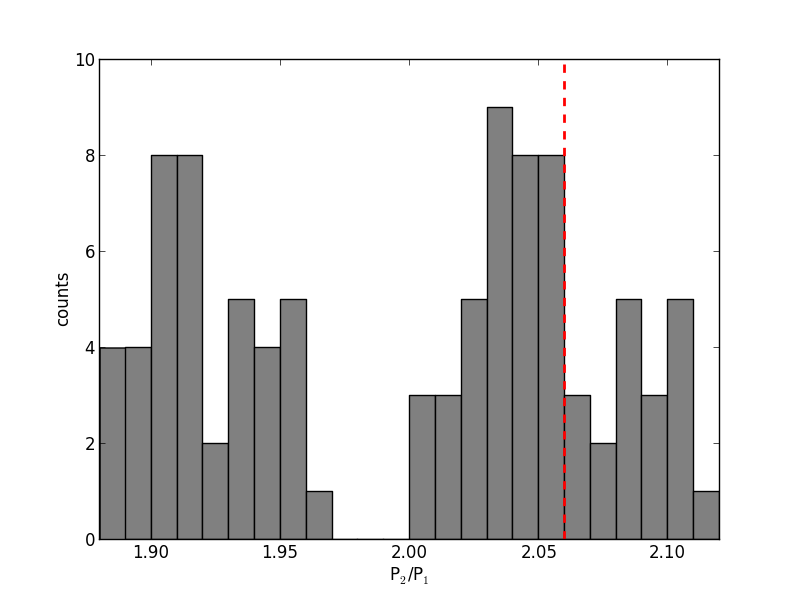
\includegraphics[scale=0.49]{chap3/MMR.png}}
\caption{ \kep{} systems close to 2:1 MMR. A statistical excess is present just wide of the 2:1 MMR, and appears to decline beyond $6\%$ of the resonance, as marked by a red dotted line. 
 }
\label{fig:MMR}
\end{figure}

We contribute to this debate by developing optimistic theoretical estimates for the evolution of planets away from resonance, and compare these estimates to N-body simulations. 
We then make a statement about the likelihood of tides to explain near-resonant pairs. 
We focus on \kep{} systems within $6\%$ of the 2:1 MMR, which appears to be the natural cutoff for this statistical excess, as shown by a dotted line in Figure~\ref{fig:MMR}. 
Using this sample we will calculate the minimum required initial eccentricity to explain their current positions, given that they started in MMR and evolved under the influence of tides alone. 
In addition, we present numerical findings of {\it resonant tugging}, an effect which prevents the evolution of planets away from MMR when eccentricity is high, making it significantly more difficult to achieve the observed spacings seen today. 
Resonant tugging does not appear to have been extensively studied/accounted for in this field due to the fact that most analysis of planets in resonance have worked in the $e \ll 1$ limit, and we find that resonant tugging exclusively affects planets in MMR with moderate to high~$e$. 

Our paper is organized as follows -- in Section~\ref{sec:meth} we outline our theoretical and numerical framework, in Section~\ref{sec:results} we present the main findings of this paper, in Section~\ref{sec:Discussion} we present a discussion and conclude in Section~\ref{sec:Conclusion}.

%%%%%%%%%%%%%%%%%%%%%%%%%%%%%%%%%%%%%%%%%%%%%%%%%%%
%%%%%%%%%%%%%%%%%%%%%%%%%%%%%%%%%%%%%%%%%%%%%%%%%%%
%%%%%%%%%%%%%%%%%%%%%%%%%%%%%%%%%%%%%%%%%%%%%%%%%%%
\section{Methods}
\label{sec:meth}
%%%%%%%%%%%%%%%%%%%%%%%%%%%%%%%%%%%%%%%%%%%%%%%%%%%
\subsection{Theory}
\label{sec: Theory}
The equations widely used to describe the evolution of planets under the influence of tides are \citep[e.g.][]{Barnes2008, LithwickWu2012,Lee2013}:
\begin{equation}
\dot{e} = -\frac{9}{2}\pi \frac{k}{Q} \frac{1}{m_p} \sqrt{\frac{GM^3}{a^3}} \left(\frac{r_p}{a} \right)^5 e
\label{eq:tidee}
\end{equation}
\begin{equation}
\dot{a} = -9\pi \frac{k}{Q} \frac{1}{m_p} \sqrt{\frac{GM^3}{a^3}} \left(\frac{r_p}{a} \right)^5 e^2 a,
\label{eq:tidea}
\end{equation}
where $a$ is the semi-major axis, $e$ is the eccentricity, $k$ is the planet's Love number, $Q$ is the planet's \textit{tidal quality factor} \citep{Goldreich1966}, $m_p$ and $r_p$ are the planet's mass and radius, respectively, $M$ is the stellar mass, and $G$ is the gravitational constant. 
From Eqs.~\ref{eq:tidee} and~\ref{eq:tidea} it follows that $\dot{e}$ and $\dot{a}$ are related by:
\begin{equation}
\frac{\dot{a}}{a} = 2e\dot{e}
\label{eq:LiWu}
\end{equation}

Which arises from conservation of orbital angular momentum.
We are interested in finding a relationship between the total migration of the system and its state variables (such as $a$ and $e$), which can be obtained by integrating Eq.~\ref{eq:LiWu}: 
\begin{equation*}
\int_{a_f}^{a_i} \frac{da}{a} = 2\int_{e_f}^{e_i} ede
\end{equation*}
\begin{equation}
a_f  = a_i \exp(- e_i^2 + e_f^2),
\label{eq:ae}
\end{equation}
where subscripts $i$ and $f$ refer to the initial and final states, respectively. 

Eq.~\ref{eq:ae} is surprisingly simple -- if we know the initial states $e_i$ and $a_i$ of a planetary body, as well as the final eccentricity $e_f$, we can predict its final position. 
Eq.~\ref{eq:ae} is independent of tidal response parameters ($k$, $Q$), the length of time considered, the mass and radii of the star/planet, etc. 
These additional factors affect the timescale by which the body arrives at its final position, $a_f$, but not the final position of the body itself. 

Let us measure the spacing of a planet pair close to a $j:j+1$ MMR by defining 
\begin{equation}
\Delta \equiv \frac{P_{out}}{P_{in}} - \frac{j+1}{j},
\label{eq:Delta}
\end{equation}
where $P$ is the orbital period, and the subscripts $in$ and $out$ refer to the inner and outer planet, respectively. 
For the 2:1~MMR, $j= 1$. 
This definition of $\Delta$ is the same as \citet{Lee2013}, and twice the value used by \citet{LithwickWu2012}. 

Using the fact that $P \propto a^{3/2}$, and substituting Eq.~\ref{eq:ae} into Eq.~\ref{eq:Delta}, we recast $\Delta$ in terms of $a_i$ and $e_i$ for the near resonant pair (setting $j=1$):
\begin{equation}
\Delta = \left(\frac{a_{out,f}}{a_{in,f}} \right)^{3/2} - 2
\label{eq:DeltaInitial}
\end{equation}
\begin{equation*}
\Delta = \left(\frac{a_{out,i}\exp(-e_{out,i}^2 + e_{out,f}^2)}{a_{in,i}\exp(-e_{in,i}^2 + e_{in,f}^2)} \right)^{3/2} - 2
\end{equation*}
We make the assumption that $e_{out,i} \approx e_{out,f}$~(see Section~\ref{sec:Discussion} for a discussion).
After simplifying, we get:
\begin{equation}
\Delta = \left(\frac{a_{out,i}\exp(e_{in,i}^2 - e_{in,f}^2)}{a_{in,i}} \right)^{3/2} - 2.
\label{eq:DeltaFinal}
\end{equation}
Thus, Eq.~\ref{eq:DeltaFinal} relates the final spacing of the system, $\Delta$, to the initial conditions of the system ($a_i$ and $e_i$) and the final eccentricity of the inner planet, $e_{in,f}$.
Eq.~\ref{eq:DeltaFinal} assumes that the angular momentum of each individual planet is conserved, which in general is not true for multi-planet systems (only total angular momentum is).
Other works \citep{LithwickWu2012,Batygin2013} have accounted for this fact, resulting in more accurate equations for the evolution of a planet pair.
We now aim to compare Eq.~\ref{eq:DeltaFinal} to numerical simulations, and estimate its accuracy for \kep{} systems with $\Delta < 0.06$ of the 2:1 MMR. 
We first outline our experimental setup.

%%%%%%%%%%%%%%%%%%%%%%%%%%%%%%%%%%%%%%%%%%%%%%%%%%%
\subsection{Experimental Setup}
\label{sec:expsetup}
Numerical simulations are carried out using the Wisdom $\& $ Holman integration scheme \citep{Wisdom1991}, implemented via REBOUND \citep{Rein2012}. 
Our sample consists of \kep{} systems near the 2:1 MMR with $\Delta < 0.06$, which we call \textit{near-resonant pairs}.
Our choice of $\Delta < 0.06$ stems from a natural cutoff where the excess of near-MMR ends, as shown in Figure~\ref{fig:MMR}. 
We exclude near-resonant pairs interior to the 2:1 MMR, since tidal forces appear only to increase planet separation with time \citep[e.g.][]{LithwickWu2012}.
In addition, we also exclude near-resonant pairs that are \textit{complex}. 
By complex, we mean dynamically involved in an additional (near) resonance (e.g. Laplace resonance), and/or containing an additional planet orbiting between the near-resonant pair. 
Our exclusion of complex resonant systems decreases the number of \kep{} systems by 6.
Lastly, we also remove the Kepler-11 system, which does not contain a complex resonance, but does go unstable on short ($\sim$Myr) timescales when placed into resonance. 
This leaves us with 27 \kep{} systems, and their properties are displayed in Table~\ref{tab:kepsys}.
We remind the reader that for each \kep{} system we simulate the entire system, not just the near-resonant planets. 

Many \kep{} planets do not currently have measured mass values, so we assign planet masses using Eq. 3 from \citet{Weiss2014} for planets $r_p < 4 r_{\oplus}$:  $(m_p/m_{\oplus}) = 2.69(r_p/r_{\oplus})^{0.93}$, and assume a density of Jupiter for planets $r_p > 4r_{\oplus}$.  
In addition, we also input mass values from the transit-timing variation study of \citet{Hadden2014} where applicable. 
For stars without measured stellar masses, we assume $M/M_{\odot} = (R/R_{\odot})^{1.25}$, derived from \cite{Demircan1991}.
For simplicity, we also assume that the inclination of our \kep{} planets is zero.

We assign k/Q values following a similar prescription as \cite{Lee2013} by assigning the most generous values possible. For Earth-like rocky planets, k/Q($r_p/r_{\oplus} < 2$) = 1/40, for planets smaller than Jupiter, k/Q($2 < r_p/r_{\oplus} < 10$) = 1/22000, and for Jupiter-sized giant gaseous planets, k/Q($r_p/r_{\oplus} > 10$) = 1/54000. 

To speed up simulation time, we increase $k/Q$ by a factor of $A_{k/Q}$ (or alternatively this could also be interpreted as increasing tidal strength). 
This tactic has been used by other scientists \citep[e.g.][]{Delisle2014}, and is valid as long as $\tau_e$ is much longer than the planet's eccentricity libration time.
We simulate our \kep{} sample for 50 Myr, and use $A_{k/Q} = 200$, giving a total simulation time of $T = 10$ Gyr.

To begin our simulations, we place each planet at a distance of 1.15$a_{obs}$, where $a_{obs}$ is the observed semi-major axis value from the \kep{} catalog, and assign $e_i = 0.01$. 
We then migrate each planet (in a type-I fashion) back to its original starting position $a_{obs}$ except for of the outer near-resonant planet, which instead migrates a distance of $a_{obs} + \Delta$, forcing the near-resonant pair into a 2:1 MMR.

Each planet migrates for time $t_{mig}$ at rate $\dot{a} = an\mu^{4/3}/C$, where $n$ is the mean motion of the inner planet, $\mu$ is the planet/star mass ratio, and $C$ is a constant. 
Lower values of $C$ cause the outer planet to encounter the MMR sooner, allowing time for both planets to migrate together in resonance, which increases eccentricity to a desired value \citep{Lee2002}. 
For the restricted 3-body problem \citet{Goldreich2014} guarantee capture into resonance if $C_{out} > 3.75$, $e_{in} < (\mu_{out}/j)^{1/3}$ but we use a more conservative value of $C_{out} = 6$ as well as perform numerical tests to ensure that overstabilities do not occur on Myr timescales. 

Defining $K \equiv \frac{\dot{e_i}/e_i}{\dot{a_i}/a_i}$, we use a default $K = 100$ when migrating planets into resonance but also experiment with $K = 10$. 
$K$ (along with $m_p/M$) affects the resulting equilibrium eccentricity, but does not affect tidal evolution, and thus does not affect our main conclusions. 
At this point, initial eccentricities of our simulated \kep{} systems range from $0.05 < e_i < 0.25$, depending on the value of $C$, $K$, etc.

After time $t_{mig}$, migration is quenched over a timescale of $t_{mig}/3$ by letting $\tau_a \rightarrow \infty$ and $\tau_e \rightarrow \infty$, where $\tau_a \equiv - a/\dot{a}$ and $\tau_e \equiv - e/\dot{e}$.
It is at this point that tides are turned on, and the system evolves under the influence of Eq.~\ref{eq:tidee} and \ref{eq:tidea} for the remainder of the simulation. 

%%%%%%%%%%%%%%%%%%%%%%%%%%%%%%%%%%%%%%%%%%%%%%%%%%%
%%%%%%%%%%%%%%%%%%%%%%%%%%%%%%%%%%%%%%%%%%%%%%%%%%%
%%%%%%%%%%%%%%%%%%%%%%%%%%%%%%%%%%%%%%%%%%%%%%%%%%%
\section{Results}
\label{sec:results}
%%%%%%%%%%%%%%%%%%%%%%%%%%%%%%%%%%%%%%%%%%%%%%%%%%%
\subsection{Theory vs. Numerics}
\label{sec:th_v_num}
We compare our theoretical predictions of tidal evolution, $\Delta_{th}$ (Eq.~\ref{eq:DeltaFinal}), to our numerical simulations, $\Delta_{num}$ (Eq.~\ref{eq:DeltaInitial}). 
The difference, $\Delta_{num} - \Delta_{th}$, is displayed as a solid line in Figure~\ref{fig:th_v_num}, and expressed as a cumulative distribution (CDF).
For all but 2 systems we see that $\Delta_{num} - \Delta_{th} < 0$, indicating that our theoretical predictions $\Delta_{th}$ consistently over-predict our numerical results, $\Delta_{num}$. 
These 2 exceptions, Kepler-32 and Kepler-221, are expected due to the fact that $T/\tau_e \sim 1000$, which allows extensive $\Delta \propto t^{1/3}$ resonant repulsion growth \citep{LithwickWu2012} in time $T$ which is not accounted for in Eq.~\ref{eq:DeltaFinal}.
Otherwise, we find that Eq.~\ref{eq:DeltaFinal} consistently overestimates the true evolution of the system.


The reason for this $\Delta_{num} - \Delta_{th} < 0$ trend is due to \textit{resonant tugging}, an effect present in the numerics but not captured by our theoretical predictions.
Resonant tugging acts to keep planets closer together than theory would predict. We explore resonant tugging in the next section. 

\begin{figure}
\centerline{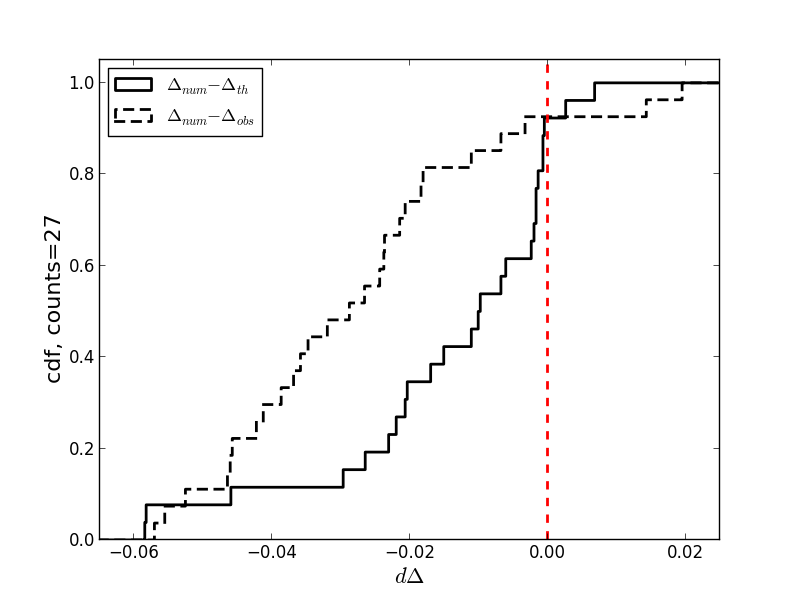
\includegraphics[trim=0cm 0cm 0.5cm 1cm, scale=0.48]{chap3/dDelta.png}}
\caption{Cumulative distribution function (CDF) of our results. The solid line shows $\Delta_{num} - \Delta_{th}$, the difference between the theoretical and simulated planet separations after $T$ = 10 Gyr. The dashed line shows $\Delta_{num} - \Delta_{obs}$, the difference between our numerical simulations and the observed \kep{} spacing.
}
\label{fig:th_v_num}
\end{figure}

For the same simulations we also plot $\Delta_{num} - \Delta_{obs}$ as a dashed line in Figure~\ref{fig:th_v_num}, which is the difference between our numerical results, $\Delta_{num}$, and the observed spacing of \kep{} planets seen today, $\Delta_{obs}$ (Eq.~\ref{eq:Delta}). 
As is clearly shown, $\Delta_{num} - \Delta_{obs} < 0$ for all but two systems, suggesting that tides alone cannot explain the observed spacing of \kep{} planets.
These two exceptions are again, Kepler-32 and Kepler-221, and are exceptions for the same reason as above. 
Since $\Delta_{obs} = 0.038$ and $0.035$ for Kepler-32 and Kepler-221, respectively, using a lower $\Delta$ cutoff for our \kep{} sample (e.g. $\Delta_{obs} < 0.03$) would not have changed our result that tides cannot explain near-resonant pairs.

Although highly suggestive, this result does not conclusively disprove tides as the primary evolving mechanism, since higher $e_i$ could cause more migration in time $T$ (see Eq.~\ref{eq:ae}), and the median eccentricity for our simulations is $e_{in,i} = 0.14$. 
Higher values of $e_{in,i}$ are possible. 
Instead of numerically exploring every possible $e_{in,i}$ value, however, we instead reverse the argument in Section~\ref{sec:mine} and calculate the minimum $e_{in,i}$ required to explain $\Delta_{obs}$.
First, however, we explore resonant tugging. 

%%%%%%%%%%%%%%%%%%%%%%%%%%%%%%%%%%%%%%%%%%%%%%%%%%%
\subsection{Resonant Tugging}
\label{sec:restugg}
\textit{Resonant tugging} affects planets in MMR subjected to energy dissipation (e.g. tidal), with moderate to high eccentricity. 
When these conditions are met and the inner planet migrates inwards (trying to leave the resonance) it tugs the outer planet inwards along with it, transferring dissipative forces from the inner to the outer planet.
The result is that the inner planet migrates less than expected, the outer planet migrates more than expected, and the planets are closer together than theory would have predicted.

Figure~\ref{fig:repulse} illustrates resonant tugging for a pair of $m = 10^{-4}M$ planets in MMR.  
For the black curve $e_{in,i} = 0.125$, for the grey curve $e_{in,i} = 0.018$, and otherwise the initial conditions of each test case are the same.
In both cases we allow \textit{only the inner planet} to evolve under the influence of tides.
The top and bottom panels show the period evolution of the outer and inner planets, respectively, and the dotted curve in the bottom panel shows evolution of the inner planet in the absence of the outer planet (also $e_{in,i} = 0.125$).

Resonant tugging is exhibited in the first 0.5 Gyr of evolution for the black curve, showing how tidal forces affecting the inner planet also affect the outer planet by dragging it inwards too. 
Comparing the solid and dotted black curves in the bottom panel of Figure~\ref{fig:repulse}, we see that in the presence of the outer planet, the inner planet migrates much less than expected due to resonant tugging. 
Since the outer planet has also migrated inwards more than expected, the result is that $\Delta_{black}$ has grown very little over the first 0.5 Gyr of evolution ($\Delta_{black} = 0.004$ after 0.5 Gyr). 

Within the framework of resonant tugging, the outer planet can be thought of as a massive anchor -- as $m_{out} / m_{in} \rightarrow \infty$ the inner planet has an increasingly difficult time migrating both bodies inwards, leading to a pair of (relatively) stationary planets. 
Conversely, as $m_{out} / m_{in} \rightarrow 0$ the inner planet has an easier time migrating both bodies inwards, and the trajectory of the inner planet will approach its single-planet trajectory (i.e. the dotted black line in Figure~\ref{fig:repulse}).

\begin{figure}
\centerline{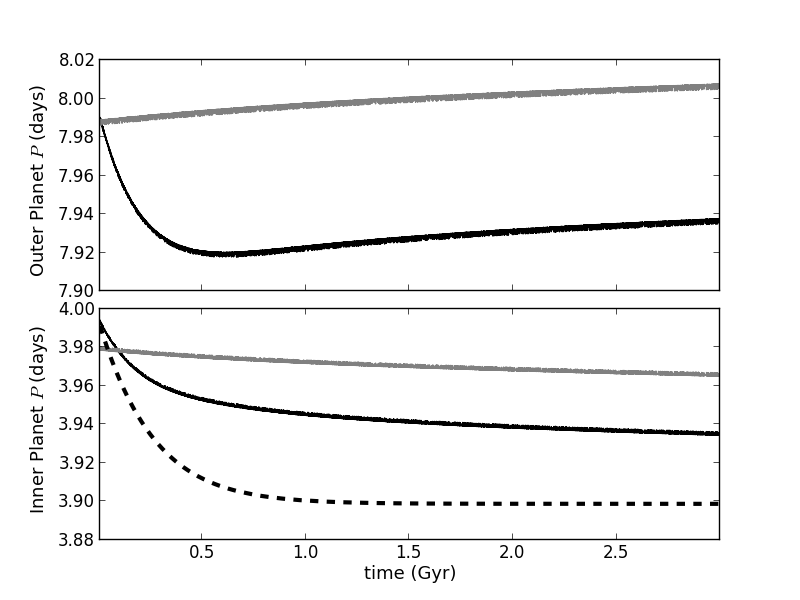
\includegraphics[trim=0cm 0cm 1cm 1cm, scale=0.48]{chap3/tugg_v_repulse_July20.png}}
\caption{ Two test cases illustrating resonant tugging and repulsion.
The top and bottom panel shows the period evolution of the inner and outer planet, respectively.
For the black curve $e_{in,i} = 0.125$, while for the grey curve $e_{in,i} = 0.018$. 
The dotted black curve shows the numerical trajectory of the inner planet ($e_{in,i} = 0.125$) in the absence of the outer planet.
}
\label{fig:repulse}
\end{figure}

We now briefly contrast resonant tugging from resonant repulsion \citep[first described by][]{LithwickWu2012}.
Qualitatively, the two main differences between resonant tugging and resonant repulsion are:
\begin{enumerate}
\item Resonant tugging exclusively affects planets in resonance (resonant angle(s) librating) with moderate to high eccentricity, while resonant repulsion affects planets both in and close to resonance, and is most noticeable in the $e \ll 1$ limit. 

\item Resonant tugging decreases $a_{in}$ and decreases $a_{out}$, while resonant repulsion decreases $a_{in}$ and increases $a_{out}$. 
\end{enumerate}

These two differences are illustrated in Figure~\ref{fig:repulse}.
The grey curve, which has low initial eccentricity ($e_{in,i} = 0.018$) exhibits pure resonant repulsion -- a decrease in $a_{in}$ and an increase in $a_{out}$, while the black curve first exhibits a shorter period of resonant tugging followed by resonant repulsion.
The transition from resonant tugging to resonant repulsion for the black curve occurs after 0.5 Gyr, when the eccentricity of the inner planet has dropped to a low ($e_{in} = 0.035$) value.

In Figure~\ref{fig:repulse}, after $\sim1$ Gyr, $\Delta_{black} < \Delta_{grey}$, but $\dot{\Delta}_{grey} = \dot{\Delta}_{black}$, showing how resonant tugging can permanently stunt the growth of $\Delta$.
We also see for the black curve that $a_{out,f} < a_{out,i}$, and it is only after many $\tau_e$ timescales that the outer planet can recover (or exceed) its initial position via resonant repulsion. 
Furthermore, since to first order (when $T/\tau_e \ll 1000$) $\dot{\Delta} \propto \tau_{a,in} \propto e_{in,i}^2$ one would naively expect the black curve to experience $e^2$ more $\Delta$ growth in time $T$, yet we actually find $\Delta_{black} < \Delta_{grey}$, illustrating just how significant resonant tugging can be.
This means that the high eccentricity tidal mechanism suggested by \citet{Delisle2014} does not work for planets in resonance, since (contrary to expectation) high eccentricity actually stunts the growth of $\Delta$, not accelerates it. 

The results shown in Fig.~\ref{fig:th_v_num} are due to resonant tugging, and is supported by the fact that for every simulated \kep{} system we find $a_{out,f} / a_{out,i} < 1$. 
Since resonant repulsion can only increase $a_{out}$ (as shown in Fig.~\ref{fig:repulse}), $a_{out,f} / a_{out,i} < 1$ can only be due to resonant tugging since inward tidal migration is a negligible contribution for the outer planet.
The analytic aspects of resonant tugging will be studied in more depth in future works.

%%%%%%%%%%%%%%%%%%%%%%%%%%%%%%%%%%%%%%%%%%%%%%%%%%%
\subsection{Minimum Eccentricity to Explain $\Delta_{obs}$}
\label{sec:mine}
Since we found in Section~\ref{sec:th_v_num} that $\Delta_{th}$ consistently over-predicts the amount of tidal migration (due to resonant tugging), we can use it as an upper limit predictor of tidal evolution, assuming that near-resonant pairs started in 2:1 MMR and evolved to their present locations. 
Starting from Eq.~\ref{eq:LiWu}, and using the same logic as Section~\ref{sec:th_v_num} we calculate the minimum eccentricity required by the inner planet to achieve the observed spacing seen today, $\Delta_{obs}$, after $T$ years (see Appendix~\ref{app:min_e} for detailed calculations):
\begin{equation}
e_{in,i} = \sqrt{\frac{\ln[(\frac{a_i}{a_f})_{out} (\frac{\Delta_{obs} + 2}{2})^{2/3}]}{1 - \exp(-2T/\tau_{e,in})}}
\label{eq:emin}
\end{equation}
Thus, for a pair of planets starting in 2:1 MMR, if we know the observed spacing today, $\Delta_{obs}$, the number of $\tau_{e,in}$ damping timescales in time $T$, and estimate the amount of migration done by the outer planet in time $T$, $(a_i /a_f)_{out}$, we can calculate the {\it minimum} initial eccentricity that the inner planet must have in order to arrive at the current spacing, $e_{in,i}$. 
Since we assume a starting position of exact 2:1 commensurability, Equation~\ref{eq:emin} is only tailored for $\Delta_{obs} > 0$. Tides cannot decrease planet spacing over time.

\begin{figure}
\centerline{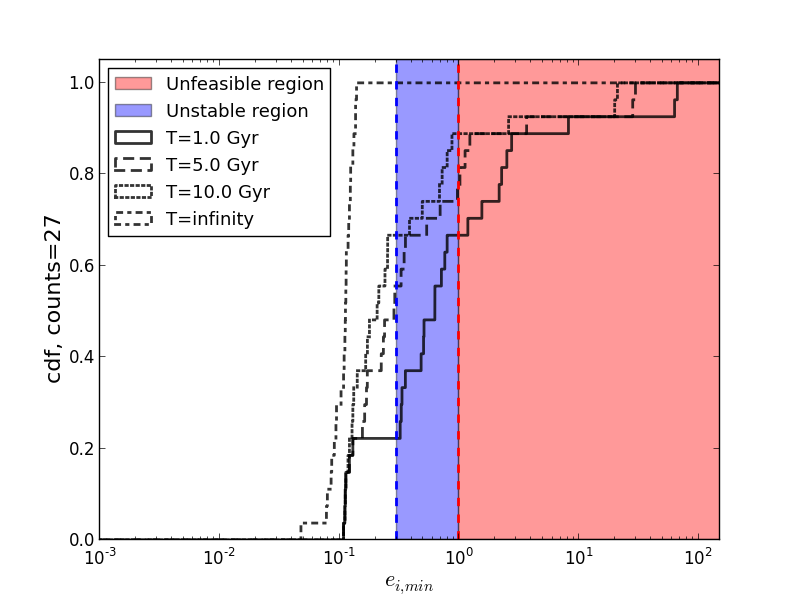
\includegraphics[trim=0cm 0cm 1cm 1cm, scale=0.48]{chap3/emin_Tconstraint.png}}
\caption{Three CDFs showing the theoretical minimum eccentricity required by the inner planet in order to achieve the observed $\Delta$ spacing seen by \kep{} planets today. The solid, dashed, dotted lines represent $T = 1, 5, 10$ Gyr tracks, respectively, while the dash-dotted line represents $T \rightarrow \infty$. In all calculations we assume the outer planet remains stationary, i.e. $(a_i /a_f)_{out}$ = 1. The red shaded region marks the unphysical region where the eccentricity is larger than unity. The blue region marks the region where most systems undergo a dynamical instability. }
\label{fig:emin}
\end{figure}

Figure~\ref{fig:emin} shows CDFs of Eq.~\ref{eq:emin} applied to our \kep{} sample for $T$ = 1 (solid), 5 (dashed), and 10 (dotted) Gyr with the outer planet remaining stationary, i.e. $(a_i /a_f)_{out} = 1$ (see Section~\ref{sec:Discussion} for a discussion).
In addition we plot a $T \rightarrow \infty$ curve as a dash-dotted line, which the other curves converge to.
The shaded red region marks where $e_{in,i} \geq 1.0$, while the blue marks an unstable region where eccentricities are unlikely to exist.
We construct the blue region by numerically finding the maximum eccentricity allowed before $> 50\%$ of our \kep{} systems go unstable within 2 Myr (see Appendix~\ref{app:emax} for details). 
We find this maximum eccentricity to be $\approx 0.3$ (the left boundary of the blue shaded region in Figure~\ref{fig:emin}).

The three $T < \infty$ curves in Figure~\ref{fig:emin} lie largely in the red and blue shaded regions, indicating that the required eccentricities to explain $\Delta_{obs}$ are unreasonable. 
We thus conclude that most \kep{} systems cannot be explained by tides alone.
Even for the $T=10$ Gyr curve, an optimistic estimate for the age of many \kep{} systems, about $35\%$ of systems still cannot be explained due to tides alone. 
Clearly, another mechanism is needed to explain the near-resonant 2:1 MMR pairs.

%%%%%%%%%%%%%%%%%%%%%%%%%%%%%%%%%%%%%%%%%%%%%%%%%%%
%%%%%%%%%%%%%%%%%%%%%%%%%%%%%%%%%%%%%%%%%%%%%%%%%%%
%%%%%%%%%%%%%%%%%%%%%%%%%%%%%%%%%%%%%%%%%%%%%%%%%%%
\section{Discussion}
\label{sec:Discussion}
A number of assumptions have been made in constructing Figure~\ref{fig:emin} which only strengthen our conclusion that planets close to the 2:1 MMR cannot be explained due to tides alone. 

First and foremost, from Sections~\ref{sec:th_v_num} and~\ref{sec:restugg} we have shown that resonant tugging causes our theoretical predictions of $\Delta$ to be overestimates, and thus Eq.~\ref{eq:emin} underestimates the minimum $e_{in,i}$ required to explain the current observed spacing. 
This discrepancy becomes most pronounced when $m_{out}/m_{in} > 1$, which is the case for many \kep{} systems in our sample.
In particular we showed that resonant tugging can stunt the evolution of planets away from MMR by roughly $e^2$ (see Sec~\ref{sec:restugg}), and this stunted evolution is not accounted for in Figure~\ref{fig:emin}.  

Second, we have assumed optimistic $k/Q$ values which allow for more migration in time $T$. 
Although \textit{some} planets could have such generous values, it is unlikely that all of them do. 
Since $\dot{a} \propto (k/Q)e^2$, as $k/Q$ decreases $e_{in,i}$ must increase in order for the planets to achieve the same observed $\Delta$ in time $T$.

Third, our estimate of $e_{max} = 0.3$ (blue-shaded region in Figure~\ref{fig:emin}) is very likely an overestimate. 
For example, \cite{Pu2015} found that the mean eccentricity of high-multiple Kepler planets must not exceed $e_{mean} = 0.02$ to guarantee long-term dynamical stability. 
Also, from simple orbit crossing arguments when $e > 0.23$ the perihelion of the outer planet crosses the aphelion of the inner planet for a 2:1 MMR, and long-term stability can no longer be guaranteed.
Even if it were possible for \kep{} systems to remain stable with high ($> 0.3$) eccentricities, it is unclear what kind of mechanism could consistently generate them for our \kep{} sample.

There are other assumptions we made throughout this paper which we now justify.
For the results presented in Fig.~\ref{fig:emin} we assumed that the outer planet remains stationary, i.e. $(a_i /a_f)_{out} = 1.00$. 
This is a reasonable assumption since, referring to our $T = 10$ Gyr numerical simulations as a benchmark, the median value of $(a_i /a_f)_{out} = 1.001 \approx 1$.
Increasing the value of $(a_i /a_f)_{out}$ shifts our CDFs in Fig.~\ref{fig:emin} further into the blue/red instability region. 

In Eq.~\ref{eq:DeltaFinal} we assumed that $e_{out,i} \approx e_{out,f}$ which essentially states that the the initial and final positions of the outer planet are the same. 
As stated in the previous paragraph, since we found numerically from our simulations that the median $(a_i /a_f)_{out} \approx 1$, this assumption is reasonable. 

In constructing Fig.~\ref{fig:emin} we have used Eq.~\ref{eq:emin}, which is Eq.~89 from \cite{Delisle2014}, who argued that for moderate to high eccentricities ($e_{in,i} \geq 0.15$), many of the near-resonant pairs could in fact be explained by tides. 
There are a number of differences between our analysis and theirs however. 
First (and most importantly), their estimates are based on theoretical predictions (i.e. resonant tugging unaccounted for), and we have shown in Section~\ref{sec:restugg} that the growth of $\Delta$ is significantly stunted when resonant tugging is accounted for, especially when $m_{out} / m_{in} > 1$.
Second, their analysis assumes that $T \rightarrow \infty$, while we restrict to $T = 1, 5$ and $10$ Gyr. 
Looking at Fig~\ref{fig:emin}, we see that the $T \rightarrow \infty$ curve tells a very different story than the $T = 1, 5$ and $10$ Gyr curves, and the conclusion of whether or not tides can explain $\Delta_{obs}$ is certainly time dependent.
Lastly, \citeauthor{Delisle2014} assumes $\Delta = 0.03$ for all systems, while we use the system specific $\Delta$ values.

As a consistency check for our results, we perform the same set of experiments (including our tests of resonant tugging) using a different version of tides, implementing them in terms of forces (as opposed to orbital elements like in Eq.~\ref{eq:tidee} and~\ref{eq:tidea}) according to \cite{Papaloizou2000}:
\begin{equation}
\vec{a}_{damp} = -2\frac{(\vec{v} \cdot \vec{r}) \vec{r}}{r^2 \tau_e}
\label{eq:tideF}
\end{equation}
where $\vec{a}_{damp}$ is the damping acceleration, $\vec{v}$ is the velocity, $\vec{r}$ is the position, $r$ is the scalar position and $\tau_e \equiv - e/\dot{e}$ as before. 
Whenever a planet receives a ``kick'' in the WH integration scheme, an additional kick of $a_{damp}$ is supplied to account for tides. 
We find our overall conclusions unaffected using this implementation of tides.

We have omitted complex resonances from our analysis because their behaviour is much more unpredictable. 
For simple resonances we found that $\Delta_{th} > \Delta_{num}$, but some complex resonances violated this relationship. 
The reasons are currently unknown, but will be more thoroughly investigated in future works. 

Lastly, it should be mentioned that spin tides were omitted from this analysis, which arise when the spin rate of the host star $\Omega_*$ is different than the mean motion $n$ of the orbiting planet (responsible for the Moon's recession from Earth over time). 
Spin rates of \kep{} stars are largely unknown, as well as the evolution of these spin rates, $d\Omega_*/dt$. 
Depending on the sign of $(\Omega_* - n)$, spin tides can induce inward or outward migration. 
It is thus a non-trivial process to determine what the affect of spin tides might be on the evolution of a system. 
The equation governing spin tide migration is \citep{SSD1999}:
\begin{equation}
\dot{a}_p = {\rm sign}(\Omega_* - n_p)\frac{3k_*}{Q_*}\frac{m_p}{M}\left(\frac{R}{a_p}\right)^5 n_pa_p
\label{eq:spina}
\end{equation}
where the subscripts $p$ and $*$ refer to the planet and star, respectively. 
We can estimate the relative strength of eccentricity tides (Eq.~\ref{eq:tidea}) to spin tides (Eq.~\ref{eq:spina}):
\begin{equation*}
\frac{\dot{a}_{ecc}}{\dot{a}_{spin}} = \frac{9\pi\frac{k_p}{Q_p} \sqrt{\frac{GM^3}{a_p^3}} \frac{e_p^2a_p}{m_p}}{ 3\frac{k_*}{Q_*}\frac{m_p}{M}\left(\frac{R}{a_p}\right)^5 n_pa_p} = 3\pi\frac{k_p}{k_*}\frac{Q_*}{Q_p}\left(\frac{M}{m_p} \right)^2 \left(\frac{r_p}{R} \right)^5 e^2
\end{equation*}
Interestingly enough, the relative strength of spin vs. eccentricity tides is independent of the semi-major axis.
Assigning typical values from \citet{WuMurray2003} for $\Omega_*$, $(k/Q)_*$, $M$ and $R$, and assuming a typical $\sim 4m_{\oplus}$ planet we get:
\begin{equation}
\frac{\dot{a}_{ecc}}{\dot{a}_{spin}} \sim 30
\end{equation}
Combining this with the fact that $\Omega_*$ and $d\Omega_*/dt$ are largely unknown for \kep{} stars, we felt justified omitting spin tides from our analysis.

\section{Conclusion}
\label{sec:Conclusion}
In conclusion, we have investigated 27 \kep{} systems containing 2:1 near-resonant pairs, and find that tides alone cannot explain their current observed spacing, $\Delta_{obs}$. 
In Figure~\ref{fig:emin} we calculated the minimum theoretical eccentricity required by the inner planet to explain $\Delta_{obs}$ and found that for a large number of systems $e_{in,i} > 0.3$, which from simple dynamical arguments is not a reasonable eccentricity for \kep{} planets to have.
Furthermore, our numerical study of resonant tugging reveals that our theoretical predictions of $e_{in,i}$ are optimistic estimates, and in cases where $m_{out}/m_{in} > 1$, significantly so.
A number of other assumptions made throughout the paper contribute to these optimistic estimates.

As a numerical compliment to our theoretical investigation, we simulated our \kep{} sample for 10 Gyr with a median eccentricity of $e_{in,i} = 0.14$, and found only two systems, Kepler-32 and Kepler-221, that migrated to $\Delta_{obs}$ (dotted line in Figure~\ref{fig:th_v_num}).
Clearly, another mechanism is required to explain the excess of \kep{} systems exterior to the 2:1 MMR. 

\section{Summary }

My Summary.
\chapter[\hermes: A hybrid integrator]{\hermes: a hybrid integrator for simulating close encounters and planetesimal migration}
\label{chap:Hermes}

\section{Chapter Overview}

We present \hermes, a new hybrid integration scheme for long-term simulations of planetary systems undergoing close encounters or planetesimal-driven migration. 
Particles are integrated using \whfast, a fast and accurate symplectic integrator, unless a close encounter occurs.
During a close encounter, a subset of particles is integrated with the high-order integrator \ias, while the rest of the particles continue to be integrated with \whfast.
We created an adaptive routine for optimizing the close encounter boundary to help maintain accuracy whilst close encounters are occurring.

Like most hybrid integrators, the switching between integrators leads to an additional, finite energy error above the standard oscillatory energy error arising from symplectic integration.
\hermes takes a more direct approach when switching between integrators than previous schemes in the literature, allowing us to analytically estimate the numerical error of our algorithm. 
Since \whfast is symplectic, \ias is accurate to machine precision and both of them are unbiased, the energy error grows sub-linearly with time under the assumption that either impact parameters are randomly distributed or close encounters are rare.

We find that \hermes provides a good balance between speed and accuracy, neither achieved by the individual symplectic or non-symplectic integrators alone.
In this Chapter, we describe the details of implementation, accuracy and performance, as well as its incorporation within the larger framework of the $N$-body package \reb. 

\section{Introduction}
\label{sec:intro}
Over the last 25 years scientists have made considerable progress integrating $N$ gravitationally interacting particles (an $N$-body system) using computational techniques. 
The most widely used integrator today for solving Solar System type problems is the Wisdom-Holman integrator \citep[hereafter WH]{Wisdom1991}, which decomposes the system's Hamiltonian, $H$, into a Keplerian and an interaction component, $H_K$ and $H_I$. 
Symplectic integrators which split the Hamiltonian in this way are known as mixed-variable symplectic integrators \citep{Wisdom1991, Saha1992}.
The system is then evolved in a second-order leapfrog manner, taking the form of $K($dt$/2) I($dt$) K($dt$/2)$, where $K$ represents evolution under $H_K$, $I$ represents evolution under $H_I$, and $dt$ is the timestep.
Although higher-order algorithms are possible \citep[e.g.][]{Yoshida1990}, the second-order WH method is an ideal balance of speed and accuracy, since the marginal increase in accuracy of higher-order methods comes at the cost of significant additional calculation. 
The evolution under the interaction Hamiltonian is trivial to solve exactly in Cartesian coordinates, whereas the evolution under the Keplerian Hamiltonian is easy to solve exactly using orbital elements. 
This algorithm therefore converts between the two coordinate systems each timestep.

Since the WH scheme breaks the evolution into operators that both derive from Hamiltonians, the algorithm is symplectic (for a review on symplectic algorithms see \citet{Yoshida1993}).
This implies that the numerical solution conserves quantities closely related to the integrals of motion, such as the total energy. 
In practice these integrals of motion are not constant, but oscillate in a bounded manner.
The relative energy error scales as $O(\epsilon dt^2)$ if the magnitude of $H_I$ remains $O(\epsilon)$ smaller than $H_K$, where $\epsilon \ll 1$ \citep{Saha1994}. 
For distant particles in non-overlapping orbits $\epsilon$ is typically much less than unity.
This is one motivation for splitting $H$ into $H_K$ and $H_I$, as it allows for longer timesteps (and thus shorter integration times) than conventional integration schemes. 
However, during close encounters, $H_I$ becomes comparable to or larger than $H_K$ causing $\epsilon$, and thus the energy error, to grow substantially. 
Therefore, despite their brief duration, close encounters typically dictate an unacceptably short timestep for the entire simulation. 
Note that it is not possible to dynamically change the timestep in the standard WH integrator as it would break time symmetry and symplecticity\footnote{If one can make the timestep choice independent of the current state, for example by using a predefined sequence of timesteps, then the integrator remains symplectic.}.

For very high accuracy integrations (with relative errors of order the machine precision), non-symplectic integrators are as good and as fast as or faster than symplectic integrators \citep{Rein2015a}.
But in most integrations, medium to low accuracy is enough to capture the qualitative evolution of a system. 
In such a case a symplectic integrator provides an advantage as the timestep can be large while keeping the numerical errors bounded.
This advantage of symplectic integrators, together with the common need to accurately resolve close encounters motivates the development of hybrid integrators that can make use of both symplectic and non-symplectic integrators.

Several hybrid integrators that make use of a (modified) WH integrator have been developed. 
The two most popular ones are \symba \citep{Duncan1998} and the hybrid integrator from the \mercury package \citep[hereafter referred to as \mercury]{Chambers1999}.

\symba decomposes the interaction potential into a series of shells around each body and uses progressively smaller timesteps for each shell to increase time resolution.
If the particles are well separated, there is only one contributing shell to the interaction term and the integrator is effectively WH.
During a close encounter the inner shells contribute to the integration using smaller timesteps to resolve the encounter.

\mercury handles close encounters by using a smooth changeover function to transfer large terms from $H_I$ to $H_K$. 
When particles are distant, interactive forces between particles are small and evaluated during $H_I$. 
When particles are close, interactive forces become large and are transferred to $H_K$, thus keeping $H_I$ small. 
This makes $H_K$ a three body problem (central body plus two particles undergoing a close encounter) which cannot be solved analytically but is straightforward to integrate numerically to high precision using a Bulirsch-Stoer routine \citep{BS1988}. 
 
In this Chapter we present a new integration method, \hermes, which borrows ideas from the integrators mentioned above, but takes a more direct approach to handling close encounters.
It combines two existing integrators, \whfast \citep{Rein2015b} 
 which is a fast and unbiased implementation of the WH method, and the high-order \ias integrator \citep{Rein2015a}. 
\hermes has been seamlessly incorporated into \reb \citep{Rein2012}, adding further flexibility to the modular $N$-body package. 

The outline for the Chapter is as follows: Section~\ref{sec:Methods} describes the algorithm for \hermes, Section~\ref{sec:Error} characterizes error, Section~\ref{sec:Examples} shows standard tests of \hermes as well as a comparison to \symba and \mercury, and we conclude in Section~\ref{sec:Conclusion}.

%%%%%%%%%%%%%%%%%%%%%%%%%%%%%%%%%%%%%%%%%%%%%%%%%%%
%%%%%%%%%%%%%%%%%%%%%%%%%%%%%%%%%%%%%%%%%%%%%%%%%%%
\section{Methods}
\label{sec:Methods}

%%%%%%%%%%%%%%%%%%%%%%%%%%%%%%%%%%%%%%%%%%%%%%%%%%%
\subsection{Particle Classification}
First we define the three different types of particles handled by \hermes: active particles, semi-active particles and test particles. 
Active particles can gravitationally affect all other types of particles, and are typically stars or planets.
Semi-active particles can affect active particles only (not other semi-active particles), and are typically asteroids, planetesimals, and other smaller objects.
Test particles are only affected by active particles and cannot affect any other particle, and are typically dust grains, rocks, small asteroids or spacecrafts. 
Figure~\ref{fig:bodies} summarizes these interactions, where arrows represent directions of gravitational influence.

\begin{figure}
\centerline{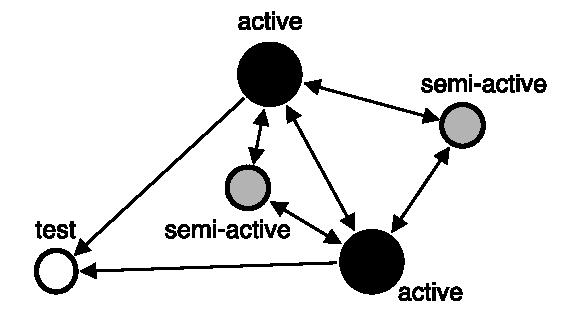
\includegraphics[scale=0.6]{chap4/images/bodies.pdf}}
\caption{A diagram illustrating how different particle types (active, semi-active, test) affect each other. Arrows indicate directions of gravitational influence.
 }
\label{fig:bodies}
\end{figure}

%%%%%%%%%%%%%%%%%%%%%%%%%%%%%%%%%%%%%%%%%%%%%%%%%%%
\subsection{Heliocentric version of \whfast}
\memoas{If cant get WHDS to work, remove this paragraph}
The original \whfast algorithm described in  \cite{Rein2015b} was implemented in Jacobi coordinates.
Jacobi coordinates lead to a better precision compared to heliocentric coordinates if orbits are well separated and do not cross each other. 
If close encounter occur, then heliocentric coordinates can help improve the integrator's accuracy.
For that reason we implemented a heliocentric version of \whfast in \reb.
We call it \whfasthelio.
We use it as the symplectic integrator in \hermes but note that \whfasthelio can also be used by itself. 
We choose the specific splitting of the Hamiltonian by \cite{Duncan1998} and \cite{Chambers1999}.
For a discussion on the different splittings, their advantages and disadvantages, see \cite{Wisdom2006}. 
For the remainder of this Chapter we will refer to \whfasthelio simply as \whfast as both integrators use the same Kepler solver.

%%%%%%%%%%%%%%%%%%%%%%%%%%%%%%%%%%%%%%%%%%%%%%%%%%%
\subsection{Algorithm}
\label{sec:Alg}
The \hermes integrator is composed of two parts, a \textit{global} simulation which contains all particles, and a \textit{mini} simulation which contains all active particles plus any semi-active or test particles involved in a close encounter.
The global simulation is integrated using \whfast, while the mini simulation is integrated using \ias. 
We first outline the overall algorithm for one timestep\footnote{We refer to the timestep that \whfast takes as $dt$. The \ias integrator chooses its own timestep which is typically smaller than $dt$.}  of length $dt$ and then describe the individual steps in more detail.

To evolve the system for a single timestep \hermes performs the following steps:
\begin{enumerate}
\item \label{step1} \textbf{Check for close encounters.} If any particle (active, semi-active, or test) has a close encounter with an active particle, then copy the particles involved in the close encounter plus all active particles to the mini simulation. 
\item \textbf{Integrate the global simulation} using the \whfast integrator for one timestep, $dt$.
\item \textbf{Integrate the mini simulation} using the \ias integrator if a close encounter was identified in step~\ref{step1}.
\item \textbf{Update the particles in the global simulation} using the mini simulation if the mini simulation was active this timestep.
\end{enumerate}

Although the algorithm is simple to write down in the above form, there are several caveats to point out.
For all particles excluding the central body, we define the parameter $\HSF$, which we dub the Hill Switch Factor. 
A spherical shell is of radius $\HSF r_H$ is constructed around each body, where $r_H$ is the Hill radius and defines the region surrounding each body where its local gravity dominates that of central body.
If the shells of any two particles overlap it is deemed a close encounter.
Since all semi-active and test particles are invisible to each other they cannot be involved in close encounters with one another.
Only particles that gravitationally interact with each other can participate in close encounters (see Fig.~\ref{fig:bodies}).
Whenever there is at least one close-encounter the mini simulation is integrated, if no close-encounters occur, the mini simulation is not active and the integrator defaults to \whfast. 
Since the central object has no Hill sphere this motivates us to define the Solar Switch Factor, $\SSF$, which only applies to the central body. 
Like $\HSF$ it also defines a spherical shell except is in units of the central object's physical radius instead of Hill radii.
Therefore, when a body passes within $\SSF r_{\odot}$ of the central object it is deemed a close encounter, where $r_{\odot}$ is the radius of the central object.

During a close encounter, \whfast still integrates all particles (including those involved in the close encounter) leading to momentarily large errors for the particles involved in the close encounter.
One might expect that this poses a real problem for the accuracy, but that is not the case, since all particles involved in the close encounter plus all active particles are overwritten at the end of the timestep using the accurate results from the mini simulation.

Unlike the global simulation, the mini simulation may take many timesteps to get from $t$ to $t + dt$.
The length of the timestep in the mini simulation is automatically determined by the \ias integrator.
During each sub-timestep the mini simulation also checks for physical collisions between overlapping particles. 

As an example of how the mini and global simulations integrate through time, consider a 2~planet, 2~planetesimal system. 
The planets are active particles and the planetesimals are semi-active particles.
Figure~\ref{fig:CE_fig} shows the distance of the planetesimals and planet~2 from planet~1 as a function of time. 
A point is plotted after every timestep in both the global and mini simulation. 
After 0.2~years, planetesimal~1 (a semi-active body) has a close encounter with planet~1 (an active body). 
At that time, the mini simulation is turned on and planetesimal~1, planet~1 the central star (not shown) and planet~2 are added to the mini simulation and integrated until 0.75~years, at which point the close encounter between planetesimal~1 and planet~1 is complete.
Planetesimal 2~on the other hand continues to be solely integrated by the global simulation (using \whfast) throughout the close encounter.
By comparing the outputs of planetesimal 2~and the other particles in Fig.~\ref{fig:CE_fig}, one can see that the mini simulation takes numerous sub-timesteps compared to the global simulation.
Since \ias is an adaptive method, it automatically chooses the appropriate timestep to resolve the close encounter with machine precision accuracy.

\begin{figure}
\centerline{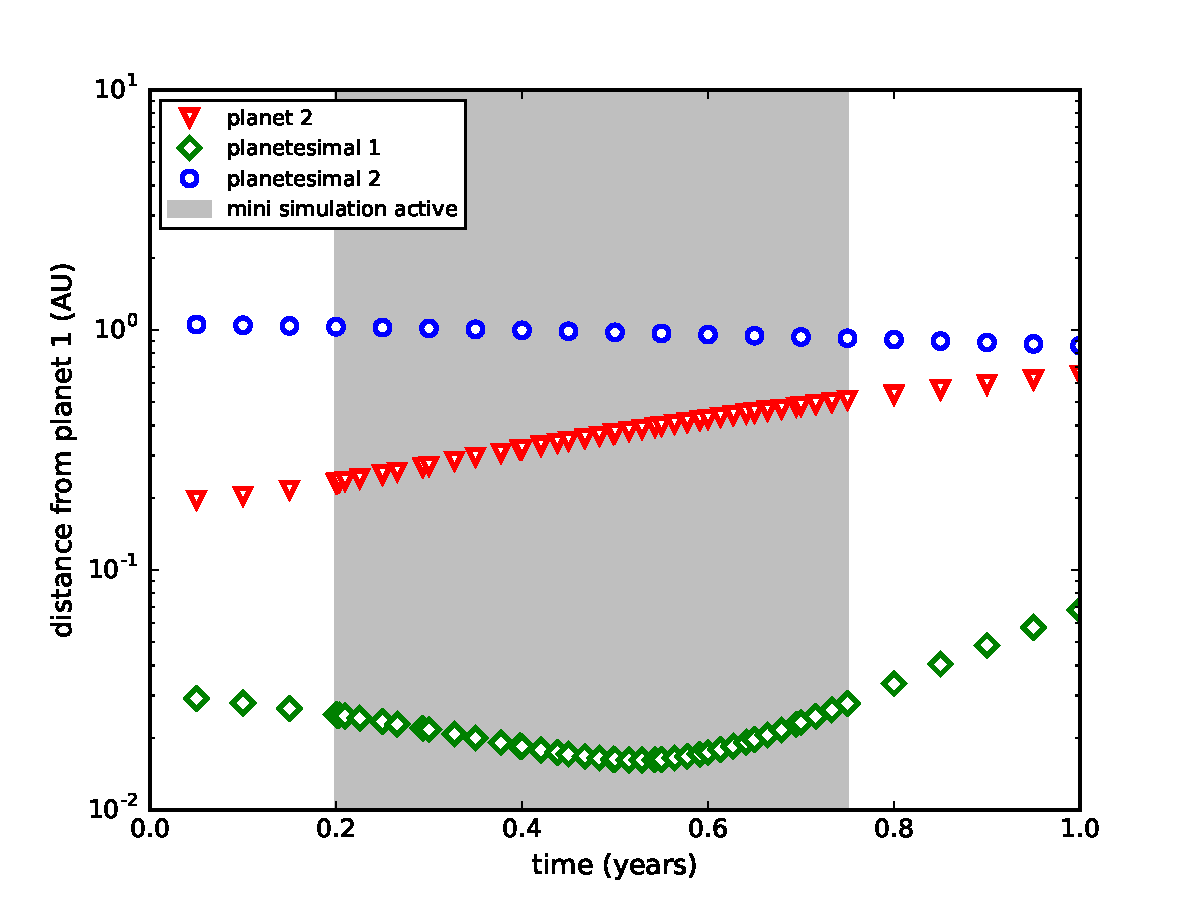
\includegraphics[scale=0.45]{chap4/images/CE_fig.pdf}}
\caption{
    A short simulation displaying the \hermes integrator for a 2~planet, 2~planetesimal system orbiting a central star. 
When active, the mini simulation takes many sub-timesteps for each $dt$ and integrates planets~1, 2~and planetesimal~1 during the close encounter between planet~1 and planetesimal~1. 
 }
\label{fig:CE_fig}
\end{figure}

We briefly discuss the speed of the algorithm.
If no particles are integrated with \ias, then the speed is effectively that of \whfast with a small overhead due to collision checks.
If all particles are integrated with \ias, then the speed is that of a simulation running only \ias, again with a small and in general negligible overhead due to collision checks. 
Consider a typical simulation of multiple active particles undergoing planetesimal migration from a large number of semi-active particles with a reasonable $\HSF$ value.
As the number of semi-active particles is increased, the ratio of the number of particles in the mini simulation, $N_{\rm mini}$, to the number of particles in the global simulation, $N_{\rm global}$, approaches a constant. 
In this limit the elapsed simulation time is linearly proportional to the number of semi-active particles in the simulation.

%%%%%%%%%%%%%%%%%%%%%%%%%%%%%%%%%%%%%%%%%%%%%%%%%%%
\subsection{Perturbative Forces in the Mini Simulation}
\label{sec:add}
One must carefully treat the forces perturbing the motions of active particles in the mini simulation. 
In the global simulation, active particles receive perturbative kicks from all semi-active particles, and it is important to reproduce these forces in the mini simulation, which only evolve a subset of particles. 
To further complicate this issue, the mini simulation takes numerous sub-timesteps for each global timestep.
In \hermes, we linearly interpolate the forces of all semi-active particles absent from the mini simulation using the initial and final values from the global simulation.
We find that interpolating the forces (rather than positions) leads to a significant speed gain without compromising noticeable accuracy.

One could argue that this process should be iterated -- the active particles will arrive at slightly different (and more accurate) final positions when integrated with the mini simulation, and thus the perturbative forces they would have induced on the semi-active particles in the global simulation would be slightly different too.
Thus if one wanted to improve the accuracy of the algorithm an iterative process could be constructed where the global and mini simulations take turns integrating for a timestep $dt$ making use of the updated positions from the previous iteration. 

However, as long as the semi-active particles have a much smaller mass than the active particles, we have found that this iterative process is unnecessary, allowing us to reduce both the computation time and algorithmic complexity.
We note that in our current non-iterative scheme, interpolating the forces between pairs of {\it active} particles introduces non-negligible numerical errors.
For that reason, all active particles are automatically added to the mini simulation during any close encounter, even if they are not involved in the close encounter themselves.

%%%%%%%%%%%%%%%%%%%%%%%%%%%%%%%%%%%%%%%%%%%%%%%%%%%
\subsection{Adaptive $\HSF$ Algorithm}
\label{sec:HSFop}
$\HSF$ and $dt$ are the most important parameters to consider when simulating a system with \hermes.
For a system free of close encounters, $dt$ alone determines the precision of the algorithm. 
However during close encounters $\HSF$ and $dt$ together determine the algorithm's precision (see Section~\ref{sec:Error}). 
Specifically, if a particle moves a distance $\sim \HSF r_H$ per timestep $dt$ the algorithm could miss a close encounter, introducing large errors into the simulation. 
In addition, an initial choice of $\HSF$ and $dt$ can become non-optimal if a system evolves significantly from its initial state. 

To aid the user in making the correct parameter choices, we have developed a simple algorithm that, given a timestep $dt$, conservatively estimates the smallest value of $\HSF$ under the condition that no close encounter is missed.
Although $\HSF$ and $dt$ both determine the precision of \hermes during a close encounter, we only optimize $\HSF$ since constantly changing $dt$ would result in non-negligible numerical errors for a symplectic integrator like \whfast.
We calculate the optimal $\HSF$ each iteration, ensuring that $\HSF$ adapts to an evolving system and guarantees that close encounters are continuously resolved.
The user is therefore only required to set the timestep $dt$ for a standard integration ($\SSF$ is set to a default value serving most purposes).
The full algorithm works as follows.

\begin{figure}
\centerline{\includegraphics[scale=0.6]{chap4/images/AutoHSF.pdf}}
\caption{Panel a. shows a regular orbit in 2D, while panel b. shows the construction of a ring by rotating the orbit's pericenter by $2\pi$.
 }
\label{fig:AutoHSF}
\end{figure}
For each body, we ignore the inclination, and marginalize over the phase and longitude of periapsis from $0$~to~$2\pi$.
As illustrated in Figure~\ref{fig:AutoHSF}, this smears out the orbit into a ring in the reference plane. 
Each ring has a maximum and minimum distance from the central object, $r_{\rm min}$ and $r_{\rm max}$.
We then check if any two interacting particles can possibly have a close encounter by comparing their $r_{\rm min}$ and $r_{\rm max}$ values.
If an intersection of two rings occurs, say for particles $i$ and $j$, we calculate their maximum relative velocity $\Delta v_{ij,\rm max}$ in the overlapping interval between the two particles.
We calculate $\Delta v_{ij,\rm max}$ as a simple overestimate rather than the true maximum in order to speed up the calculation.
As a result of ignoring the inclination and marginalizing over the phase and longitude of periastron, $\Delta v_{\rm max}$ can be calculated from just the semi-major axis and the eccentricity.
We note that we do not need to solve Kepler's equation in estimating $\Delta v_{\rm max}$.

We can then calculate $\HSF$ by taking the maximum over all interacting particle pairs (see Fig~\ref{fig:bodies}),
\begin{equation*}
\HSF = 4\;\underset{i,j}{\textrm{max}}\frac{ \Delta v_{ij,\rm max} dt}{r_{H, i} + r_{H,j}}.
\end{equation*}
The numerical constant $4$ ensures that two particles move at most one quarter of $\HSF (r_{H, i} + r_{H,j})$ in one timestep and therefore no close encounters are missed.

In practice, we also round up $\HSF$ to the nearest $1.25^x$ where $x$ is an integer to avoid continuous fluctuations in $\HSF$. 
By default, our adaptive $\HSF$ algorithm is enabled in \hermes.
Since the algorithm assumes particles move on approximately coplanar orbits, it may therefore fail at very high mutual inclinations.
We note that the above algorithm chooses the smallest value of $\HSF$ that captures all close encounters; however, small values of $\HSF$ introduce numerical errors when switching between integrators (see Section~\ref{sec:Error}).
Therefore, to avoid large errors we set a default lower limit of $\HSF=3$, which is close to the default close encounter boundary for \mercury and \symba.
The user can specify their own lower limit for $\HSF$ by setting {\sc \tt ri\_hermes.hill\_switch\_factor} at runtime. 

The adaptive $\HSF$ algorithm can be switched off by setting the variable {\sc \tt ri\_hermes.adaptive\_hill\_switch\_factor} to zero.
If the adaptive $\HSF$ algorithm is switched off, setting {\sc \tt ri\_hermes.hill\_switch\_factor} simply defines a constant value of $\HSF$ for the duration of the simulation (analogous to \mercury and \symba). 

We decided against devising a similar algorithm for $\SSF$ due to the additional difficulties that can arise. 
For example, an object in a circular orbit around a planet would be confused as a heliocentric orbit with a very high eccentricity, leading to large relative velocities and an excessive $\SSF$ value. 

%%%%%%%%%%%%%%%%%%%%%%%%%%%%%%%%%%%%%%%%%%%%%%%%%%%
%%%%%%%%%%%%%%%%%%%%%%%%%%%%%%%%%%%%%%%%%%%%%%%%%%%
\section{Error}
\label{sec:Error}
Several terms contribute to the relative energy error of an integrator \citep[e.g.][]{Rein2015a}:
\begin{equation}
E = E_{\rm floor} + E_{\rm round}  + E_{\rm bias} + E_{\rm scheme}.
\label{eq:error}
\end{equation}

$E_{\rm floor}$ is a constant due to the inability to represent numbers with arbitrary precision on a computer.  
Here we work exclusively in IEEE754 double floating point precision and thus have $E_{\rm floor}\sim 10^{-16}$. 

$E_{\rm round}$ arises when a computation is performed on two floating point numbers. 
Almost all operations (addition, multiplication, square roots) lead to a roundoff error at the level of the machine precision.
The IEEE754 standard guarantees that the round-off error in consecutive floating point operations is random, thus leading to a $\propto t^{1/2}$ growth of $E_{\rm round}$ with time.

$E_{\rm bias}$ is the error from any biased operations and grows at least as $\propto t$.
Biased operations can originate from poor implementations\footnote{For example, the expression \texttt{x*(2./3.)} multiplies $x$ by a number that is consistently slightly too big or too small when represented in binary.  By contrast, the expression \texttt{2.*(x/3.)} multiplies and divides $x$ by numbers that are exactly representable in binary and is unbiased.} or from library functions that the IEEE754 standard does not guarantee will return unbiased results\footnote{For example, the standard library function \texttt{sqrt()} returns an unbiased result whereas \texttt{sin()} returns a biased result.} .

$E_{\rm scheme}$, the final term in Eq.~\ref{eq:error}, is the error introduced by the algorithm itself. 
Typically, this quantity is bound for symplectic integrators but grows linearly with time for non-symplectic integrators.

The important question is which error term dominates, and the answer will depend on the problem at hand.
For example, if a three-body system (star and two planets) is integrated with \ias, $E_{\rm scheme}^{ias} \approx 10^{-28}$ and the dominant error term will be $E_{\rm round}$, starting at $10^{-16}$ and growing as $t^{1/2}$ \citep[see][]{Rein2015a}. 
If we instead integrate the system with \whfast, the dominant error term will be $E_{\rm scheme}$, which is determined both by the mass ratio in the system and the timestep. 
For typical parameters $E^{WH}_{\rm scheme} \sim 10^{-9}$, and only for very long simulation times ($\sim 10^{14}$ timesteps) will the growth of $E_{\rm round}$ dominate over $E^{WH}_{\rm scheme}$.
For biased implementations, $E_{\rm bias}$ will dominate the error budget at earlier times.  

For typical simulations integrated with \hermes, $E_{\rm scheme}$ will dominate. 
The WH algorithm integrates a slightly different Hamiltonian from the true Hamiltonian described by the system, leading to an error that oscillates in a bounded manner as long as the integrated Hamiltonian remains constant.
However each time a particle is transferred to or from the global simulation (see Section~\ref{sec:Alg}), the WH-integrated Hamiltonian changes, and thus the error will change too.
For a typical WH integration, working in democratic heliocentric coordinates, $E_{\rm scheme}$ is \citep[e.g.][]{Saha1994,Wisdom2006}:
\begin{equation}
E_{\rm scheme}^{\rm WH} = \frac{dt^2}{12} \left \{ \left \{H_K, H_{\beta} \right \},  0.5H_K + H_{\beta} \right \} + O(dt^4)
\label{eq:WHerr}
\end{equation}
Here $H_K$ is the Keplerian Hamiltonian, $H_{\beta} = H_C + H_I$ is the summed momentum cross-term and interaction Hamiltonians, respectively, and \{\} are Poisson brackets (the quantities are explicitly defined for a test case with three particles below). 
For large $N$-body systems, Eq.~\ref{eq:WHerr} quickly becomes very difficult to evaluate analytically. 
However, we can gain some insight by applying Eq.~\ref{eq:WHerr} to a simple system. 

\begin{figure}
\centerline{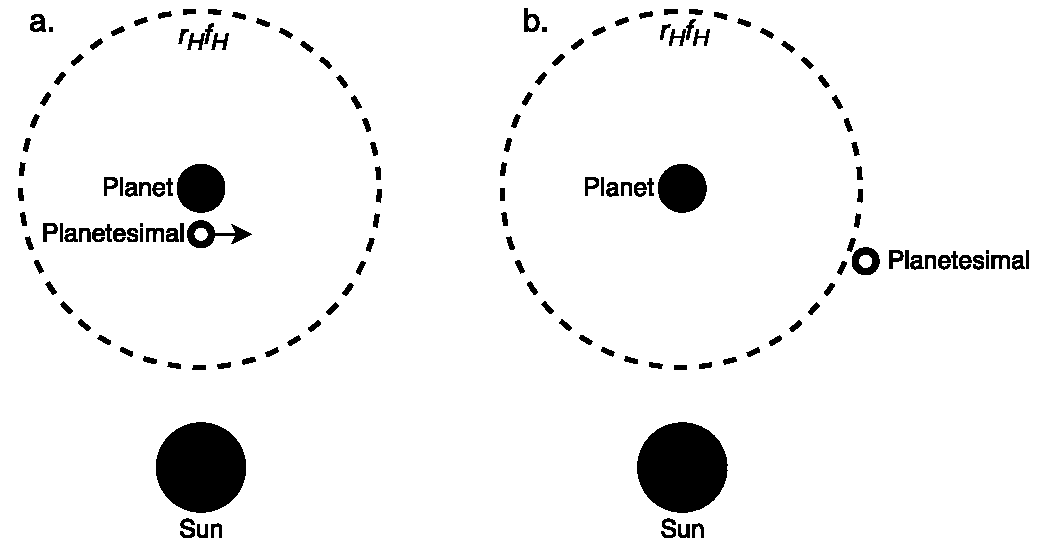
\includegraphics[scale=0.45]{chap4/images/R3B.pdf}}
\caption{Three body problem, in the reference frame of the planet. 
In a. the initial setup is shown, where the planetesimal starts near the planet, inside a sphere of radius $r_H\HSF$ and the entire system is integrated purely by \ias. 
Here the arrow indicates the initial direction of the planetesimal. 
In b. the planetesimal exits the sphere with radius $r_H\HSF$ and the system is integrated purely via \whfast, introducing a numerical error of $E_{\rm scheme}^{\rm WH}$.
}
\label{fig:R3B}
\end{figure}

We turn to a three body problem consisting of a star (active body), planet (active body) and planetesimal (semi-active body), shown in Figure~\ref{fig:R3B}.
The planetesimal is initially placed inside $\HSF$ with sufficient velocity such that the distance between the planet and planetesimal grows over time. 
While the planetesimal is inside $\HSF$ (panel a. in Fig.~\ref{fig:R3B}) the system is integrated to machine precision by \ias.
However once the planetesimal leaves $\HSF$ (panel b. in Fig.~\ref{fig:R3B}) the system switches to being integrated by \whfast, and an error of size $E_{\rm scheme}^{\rm WH}$ is introduced.

To estimate  $E_{\rm scheme}^{\rm WH}$, we start from the general Hamiltonian for an $N$-body system in Democratic Heliocentric coordinates:
\begin{equation*}
H = H_0 + H_K + H_C + H_I
\label{eq:Hbasic}
\end{equation*}
where $H_0$ is a constant describing the motion of the centre of mass along a straight line, and disappears when we evaluate Eq~\ref{eq:WHerr}. 
The remaining terms in Eq.~\ref{eq:Hbasic} take the form \citep{Duncan1998}:
\begin{align}
H_K &= \sum_{i=1}^{N-1} \frac{\bf{P}_i^2}{2m_i} - \sum_{i=1}^{N-1} \frac{Gm_0m_i}{|\bf{Q_i}|} \label{eq:H_K}\\
H_C &= \frac{1}{2m_0} \left|\sum_{i=1}^{N} \bf{P}_i \right|^2 \label{eq:H_C}\\
H_I &= -\sum_{i=1}^{N-1}\sum_{j=i+1}^{N} \frac{Gm_im_j}{|\bf{Q}_i - \bf{Q}_j|}\label{eq:H_I}
\end{align}
where the canonical coordinates $\bf{Q}$ and $\bf{P}$ are:
\begin{equation}
\bf{Q}_i = \begin{cases}
\bf{r}_i - \bf{r}_0 & \text{if } i \ne 0\\
\frac{1}{m_{\rm tot}}\sum_{j=0}^{N}m_jr_j & \text{if } i = 0\\
\end{cases}
\end{equation}
\begin{equation}
\bf{P}_i = \begin{cases}
\bf{p}_i - \frac{m_i}{m_{\rm tot}} \sum_{j=0}^{N} \bf{p}_j & \text{if } i \ne 0\\
\sum_{j=0}^{N} \bf{p}_j & \text{if } i = 0\\
\end{cases}
\end{equation}
Here $\bf{p}$, $\bf{r}$, $m$ are a particle's momentum, position and mass in any inertial frame respectively, while $G$ is the gravitational constant and $m_{\rm tot} =  \sum_{j=0}^{N} m_j$ is the total mass of the system.
$\bf{Q}_i$ are therefore heliocentric positions (with $\bf{Q}_0$ the centre of mass), while $\bf{P}_i$ are barycentric momenta (with $\bf{P}_0$ the momentum of the centre of mass).

We also further simplify the system to two dimensions by considering motion in a plane. 
One can then straightforwardly, albeit tediously, evaluate the Poisson bracket in Eq.~\ref{eq:WHerr} by plugging in Eqs.~\ref{eq:H_K}--\ref{eq:H_I} and taking derivatives with respect to all three particles. 
We make the further simplifying assumptions that $m_0 \gg m_2 \gg m_1$ and that $v_1 \approx v_2 \approx \sqrt{Gm_0/a}$, where $v$ denotes particle velocities and $a_2$ is the semi-major axis of the planet.
In addition, after solving Eq.~\ref{eq:WHerr} we set the distance of the planetesimal from the planet to $r_{H}\HSF$, where $r_{H}$ is the Hill radius of the planet. 
This is true at the moment the integration method is switched.
We are then left with a single dominating term,
\begin{equation}
\begin{split}
E_{\rm scheme}^{\hermes} \approx \frac{dt^2}{12} \frac{G^2 m_0m_1m_2}{a_2(r_{H}\HSF)^3},
\label{eq:Escheme}
\end{split}
\end{equation}
where we have ignored numerical constants of order unity.
An IPython notebook with a computer derivation is available at \url{https://github.com/silburt/hermes_ipython}.

\begin{figure}
\centerline{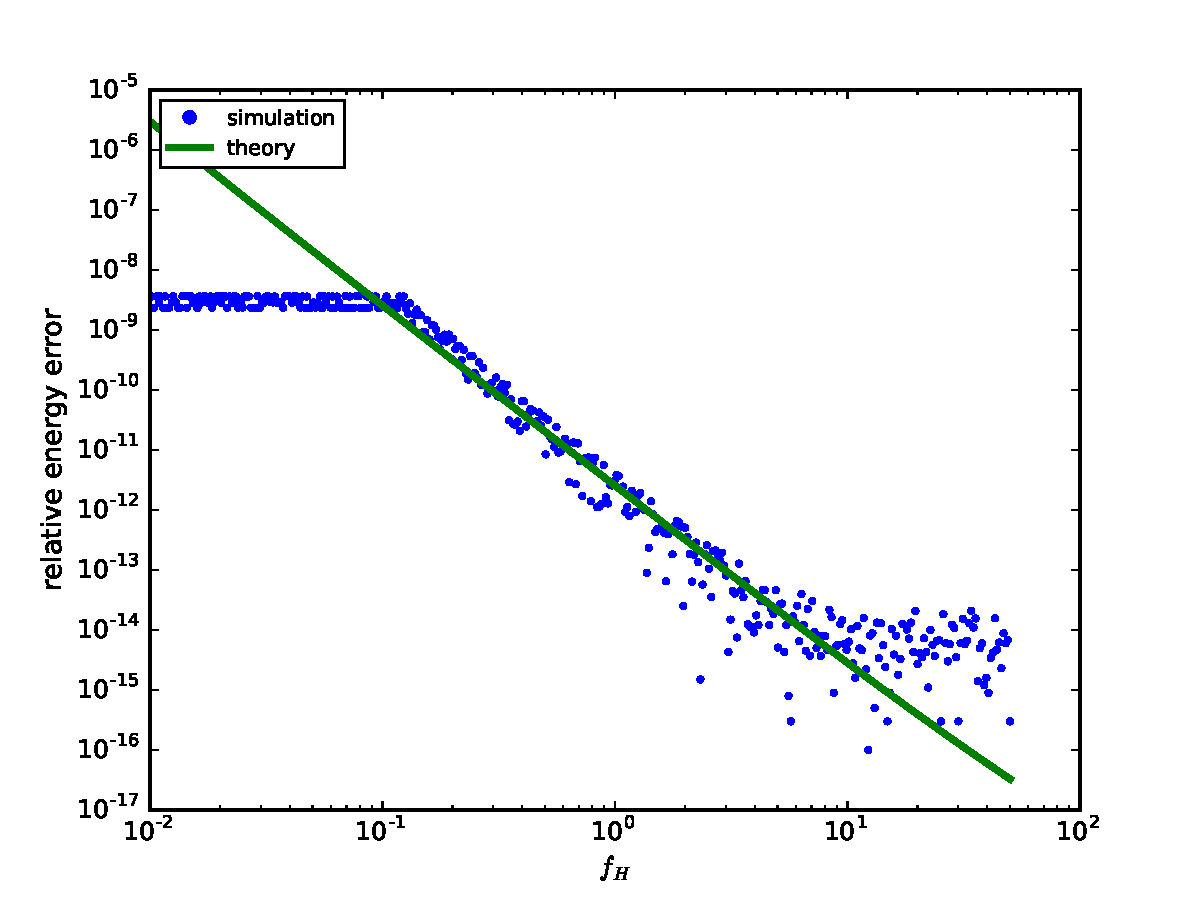
\includegraphics[scale=0.45]{chap4/images/HSR_v_dE.pdf}}
\caption{Final relative energy error as a function of $\HSF$ for a star-planet-planetesimal system. 
Blue dots are numerical simulations, the green curve is the theoretical prediction of Eq.~\ref{eq:Escheme}.
 }
\label{fig:HSFdE}
\end{figure}
We compare our theoretical predictions in Eq.~\ref{eq:Escheme} to numerical tests in Figures \ref{fig:HSFdE} and \ref{fig:dtdE}.
Our numerical setup consists of a star with mass $1M_\odot$, a Neptune mass planet on a circular orbit at $1$~AU, and a planetesimal with mass $10^{-8}M_\odot$ placed at $0.001$~AU from the planet.
To marginalize over the phase of the encounter when sampling the energy error, the initial position of the planetesimal is randomized for each realization.
In addition, the planetesimal is given a small kick equal to the escape velocity of the planet to ensure that the planetesimal-planet distance increases with time.
Each realization is simulated for 7 years.
When varying the timestep in Fig.~\ref{fig:dtdE} we use a constant $\HSF = 6$, and when varying $\HSF$ in Fig.~\ref{fig:HSFdE} we use a constant timestep of $dt = 0.058$~days.

In Figure~\ref{fig:HSFdE} one can see that the numerical tests agree with the theoretical predictions of Eq.~\ref{eq:Escheme}.
In addition, one can see the two extreme regimes on each end of the figure.
For particles starting outside the $r_H\HSF$ boundary the integrator always uses \whfast (like panel b. of Fig.~\ref{fig:R3B}), while for particles inside the $r_H \HSF$ boundary the simulation uses \ias (like panel a. of Fig.~\ref{fig:R3B}).
In Figure~\ref{fig:dtdE} one can see that the relative energy error is proportional to $dt^2$, again matching the predictions of Eq.~\ref{eq:Escheme}.
For both Fig.~\ref{fig:HSFdE} and Fig.~\ref{fig:dtdE}, we have not performed any kind of fit, we simply over-plotted Eq.~\ref{eq:Escheme} with the data from our numerical experiments. 
We have performed other suites of simulations testing how the energy error scales with all other relevant quantities (semi-major axis, planetesimal mass, planet mass, stellar mass) and find Eq.~\ref{eq:Escheme} in good agreement.
An IPython notebook for these experiments (including tests of the other relevant quantities) is available at \url{https://github.com/silburt/hermes_ipython}.

\begin{figure}
\centerline{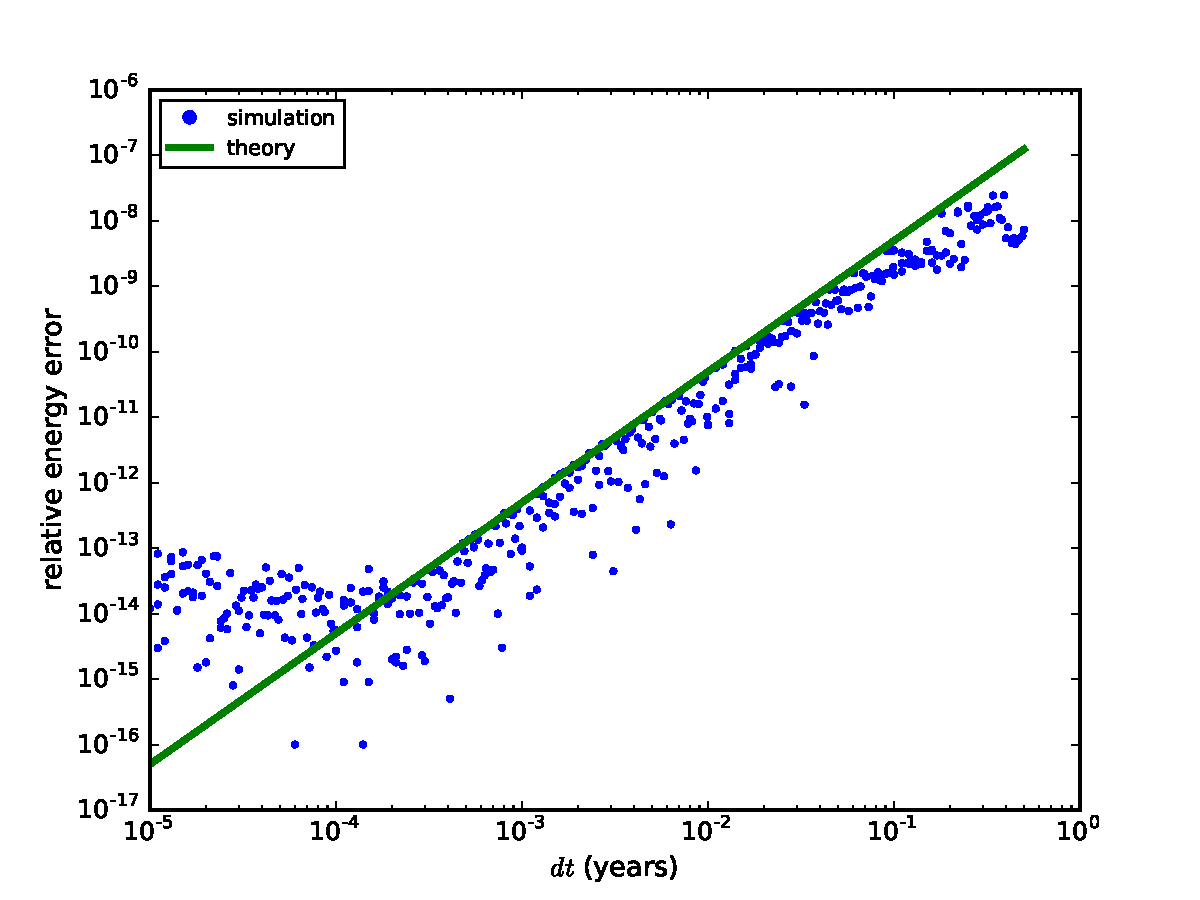
\includegraphics[scale=0.45]{chap4/images/dt_v_dE.pdf}}
\caption{Final energy error as a function of $dt$ for a star-planet-planetesimal system. 
Blue dots are numerical simulations, the green curve is the theoretical prediction of Eq.~\ref{eq:Escheme}.
 }
\label{fig:dtdE}
\end{figure}

We now extend the characterization of the error to a more realistic case with $N$ particles.
We refer to the total relative energy error for an integration as $E_{\rm scheme,tot}^{\hermes}$.
Since an error of size $E_{\rm scheme}^{\hermes}$ is introduced each time a particle leaves/enters the global simulation, the total errors should be related to the number of close encounters, $N_{\rm CE}$.
In the ideal case where the integrator is unbiased, the error $E_{\rm scheme}^{\hermes}$ introduced by each close encounter is random, and $E_{\rm scheme,tot}^{\hermes}$ will grow as a $N_{\rm CE}^{1/2}$ random walk.
However, if \hermes is biased (i.e. $E_{\rm scheme}^{\hermes}$ is not random), then $E_{\rm scheme,tot}^{\hermes}$ will grow faster than $N_{\rm CE}^{1/2}$. 

Assuming the unbiased case, $E_{\rm scheme,tot}^{\hermes}$ is equal to:
\begin{equation}
E_{\rm scheme,tot}^{\hermes} = K \cdot E_{\rm scheme}^{\hermes}  \cdot  \sqrt{N_{\rm CE}}
\label{eq:Etot}
\end{equation}
where $K$ is a constant of proportionality. 
We test Eq.~\ref{eq:Etot} against numerical tests for a Solar mass star, a Neptune mass planet on a circular orbit at $1$~AU, and a disk of 200 planetesimals located between $0.98 - 1.02$~AU.
The initial inclinations and eccentricities of the planetesimals in the disk are set to 0, while the argument of perihelion and true anomaly are drawn from a uniform distribution.
In addition, for these simulations we set $\HSF = 6$ and $dt = 0.015$ years. 
We performed numerous integrations, integrating each realization for a randomly chosen number of orbital periods between 10-1000, yielding different numbers of close encounters.

\begin{figure}
\centerline{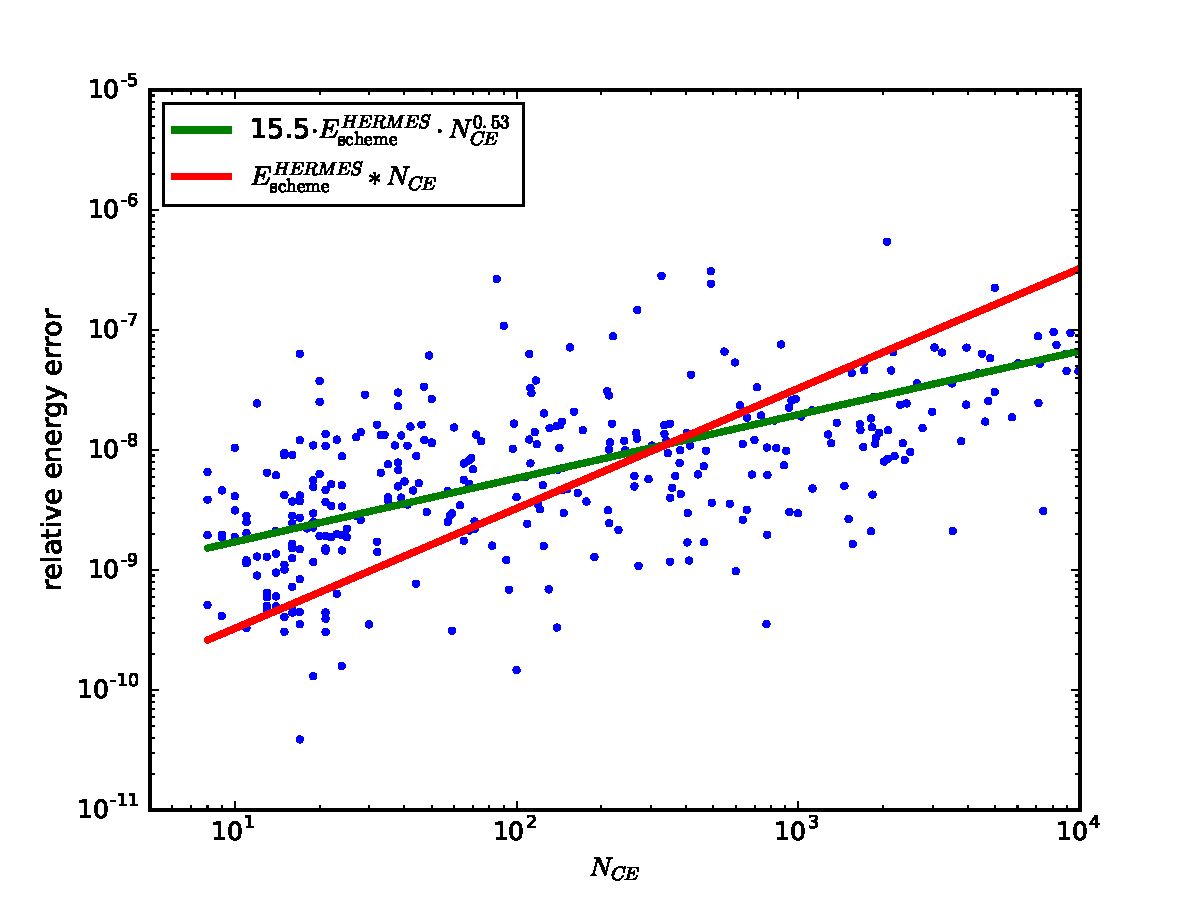
\includegraphics[scale=0.45]{chap4/images/CEvdE.pdf}}
\caption{Final relative energy error as a function of the number of close encounters, for a system composed of a star, planet and 200 planetesimals. 
Blue dots are numerical simulations, the green line is our unbiased theoretical prediction of Eq.~\ref{eq:Etot} with $K = 15$, while the red line is the biased theoretical prediction.
 }
\label{fig:HSFratio}
\end{figure}

The results are shown in Figure~\ref{fig:HSFratio}, the x-axis showing the number of close encounters during a simulation and the y-axis showing the final relative energy error for each simulation.
We fit a power-law distribution to the data using Python's Scipy Optimize Curve Fit package \citep{Scipy2016}, displayed as a green line in Fig.~\ref{fig:HSFratio}. 
The resulting fit is $E_{\rm scheme,tot}^{\hermes}= 15.5 \cdot E_{\rm scheme}^{\hermes} \cdot N_{\rm CE}^{0.53}$, so the energy growth is well approximated by Eq.~\ref{eq:Etot}. 
For reference, we plot the biased prediction of $E_{\rm scheme,tot}^{\hermes} \propto N_{\rm CE}$ as a red line.
We conclude that \hermes is unbiased for this setup.
Thus, Eq.~\ref{eq:Etot} provides an intuitive way of understanding how the error of \hermes grows without having to analytically solve Eq.~\ref{eq:WHerr} in three dimensions for $N$ particles. 

The results from Fig.~\ref{fig:HSFratio} did not allow for physical collisions between particles. When physical collision are enabled a systematic bias can be introduced. 

To see why, note that for each close encounter two contributions to the energy error arise according to Eq.~\ref{eq:Escheme}; one when the particles are transferred from the global to the mini simulation (i.e. the ingress of the close encounter) and one when the particles are transferred back from the mini to the global simulation (i.e. the egress of the close encounter).
The precise energy change depends on the specific properties of the system (phases of the orbits, angles of approach, etc.), and typically the energy changes associated with the ingress and egress of the close encounter are anticorrelated. 
As a result, no appreciable energy error is introduced by close encounters, and the energy over the course of a simulation grows as expected according to Eq.~\ref{eq:Etot}.

However, when a physical collision occurs in \hermes,  the close encounter only has an ingress, resulting in a biased growth in the energy error. 
In practice this energy bias is orders of magnitude smaller than the physical energy lost during a collision, and therefore should not interfere with the longterm evolution of a system. 
We plan to study this issue in more detail in the future. 

\section{Examples}
\label{sec:Examples}
\memoas{\hermes is well suited for a number of astrophysical problems.
For example, planets embedded in planetesimal disks are ideal for \hermes, and was the primary motivation for building this integrator.
Planet-planet scattering can also be easily simulated with \hermes, especially since our adaptive $\HSF$ algorithm (Section~\ref{sec:HSFop}) protects close encounters from being missed. 
High eccentricity cometary clouds (e.g. the Oort cloud) are also efficiently integrated with \hermes since (by enlarging $\SSF$) pericenter passages can be resolved in the mini simulation while the remainder of the orbit is integrated in the global simulation using a large timestep. 
Other examples include star clusters orbiting about a central potential, tidal migration and longterm stability of planetary systems, etc.
Many example problems can be found at \url{https://github.com/hannorein/rebound/tree/master/ipython_examples}.}
Below, we highlight just a few example problems that can be simulated with \hermes.

\subsection{Massive Outer Solar System}
Both \citet{Duncan1998} and \citet{Chambers1999} simulated the outer Solar System, but increased the masses of all planets by a factor of 50 to trigger close encounters between planets.
Analogous to \citet{Chambers1999} and \citet{Duncan1998} we use $\HSF=3$, $dt= 0.03$~yrs, and integrate the system for 1000 years. 

We perform a number of simulations of the massive outer Solar System, and find that the relative energy error stays bounded at~$\sim 10^{-7}$ for all simulations, matching the results of \citet{Chambers1999} and \citet{Duncan1998}. 

\subsection{Migration of a Planet in Planetesimal Disk \citep{Kirsh2009} }
Here we reproduce the results of \citet{Kirsh2009} for the migration of a single planet embedded in a planetesimal disk. 
In this study a 2.3$M_{\oplus}$ planet orbits a Solar mass star at $25$~AU, embedded in a disk of $\sim6\cdot10^4$~planetesimals. 
The planetesimal disk extends 10.5 AU on each side of the planet, each planetesimal has a mass 1/600th of the planet, and an overall surface density profile proportional to $a^{-1}$ is used.
The radii of all orbiting particles were determined assuming a constant density of $2~\rm{ g/cm^3}$.
The eccentricities and inclinations were drawn from a Rayleigh distribution, which is parameterized by the scale parameter $\sigma$.
For this experiment we use $\sigma_e = 0.01$, and $\sigma_i = 0.005$, where inclination is in radians.
The argument of periapse, true anomaly, and longitude of ascending node were all randomly drawn from uniform distributions over $[0, 2\pi]$.
Adopting the default settings of \citet{Kirsh2009}, we set \hermes to merge particles inelastically, set $dt=2$ years, $\HSF = 5$, $\SSF = 15$, and track the energy lost due to collisions or ejections. 
We also set {\sc \tt r->ri\_hermes.adaptive\_hill\_switch\_factor} = 1, activating the adaptive Hill switch routine (Section~\ref{sec:HSFop}).
An IPython notebook containing the code to run this example can be found at \url{https://github.com/silburt/hermes_ipython}.

We run 6 separate simulations, each for 70,000 years, and plot the results in Fig.~\ref{fig:Kirsh}.
The relevant comparison plot in \citet{Kirsh2009} is the lower right panel in Figure~3.
For all runs in both \citet{Kirsh2009} and our work the final position of the planet is between $18.5 < a < 20$ AU, and show similar evolution tracks throughout the simulation. 
The relative energy error over the course of all our simulations do not exceed $2\cdot10^{-7}$ after accounting for the energy lost in inelastic collisions. 

\begin{figure}
\centerline{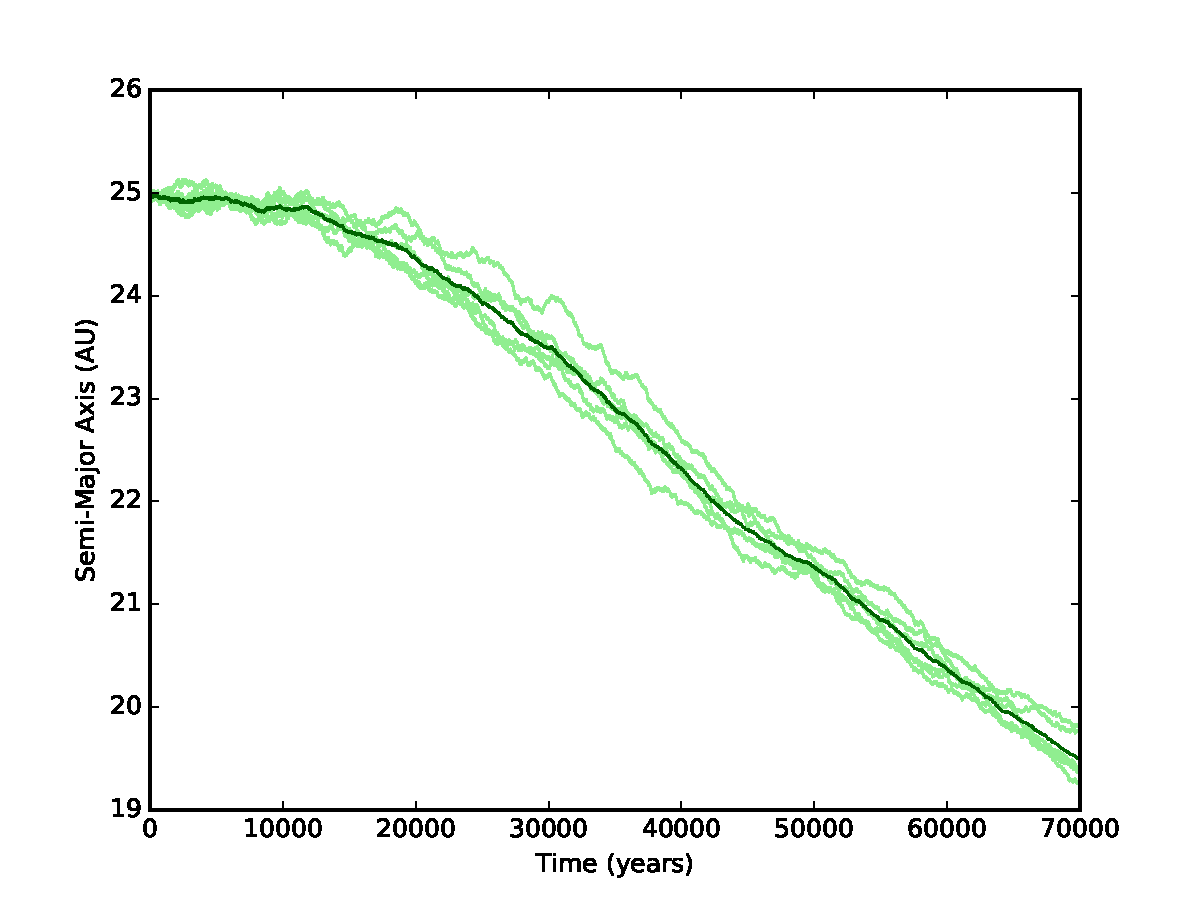
\includegraphics[scale=0.45]{chap4/images/Kirsh_avg_a.pdf}}
\caption{
Planet's semimajor axis vs. time, analogous to the numerical experiment in the lower right panel of Figure~3 from  \citet{Kirsh2009}. 
Light green lines represent individual runs, while the dark thicker green line represents the average of the individual runs. 
 }
\label{fig:Kirsh}
\end{figure}

\subsection{Comparison to \mercury and \symba -- Long Simulations}
Here we perform a set of long simulations and compare our results to \mercury and \symba.
These integrators are also capable of integrating complex $N$-body systems with close encounters, and also make use of semi-active particles.
The simulations for these tests contain a Solar-mass star, a Neptune-mass planet at $a=1$~AU and a disk of 100~semi-active planetesimals distributed according to a powerlaw between $0.8 - 1.2$~AU. 
The mass of each planetesimal is a third of a lunar mass, the eccentricities and inclinations are set to 0, and the argument of periapse, true anomaly, and longitude of ascending node were all randomly drawn from uniform distributions over $[0, 2\pi]$.
We set $dt = 0.01$, $\HSF = 3$, merge particles inelastically, and use our adaptive $\HSF$ routine (Section~\ref{sec:HSFop}). 
In addition, for all three integrators we track the energy lost due to inelastic collisions and ejections so that we can isolate the numerical energy error. 
We accomplish this by using the \texttt{eoffset} variable in \symba and \texttt{EN(3)} variable in \mercury, and calculate the relative energy error according to $(E_{i} + E_{\rm off} - E_{\rm 0})/E_{0}$, where $E_i$ is the total energy at iteration $i$, $E_0$ is the initial total energy and $E_{\rm off}$ is the energy lost due to collisions and ejections, i.e. \texttt{eoffset} in \symba and \texttt{EN(3)} in \mercury. 

We feed identical initial conditions to \symba, \mercury and \hermes, and evolve all simulations for 50 Myr. 
We run 6 simulations per integrator that differ only by the seed of the random number generator.
We average the relative energy error for these simulations to smooth out variations between individual runs.
The results are presented in Figure~\ref{fig:Np100test}.
The top panel displays the relative energy error with each integrator, while the bottom panel shows the elapsed time for each individual run.

\begin{figure}
\centerline{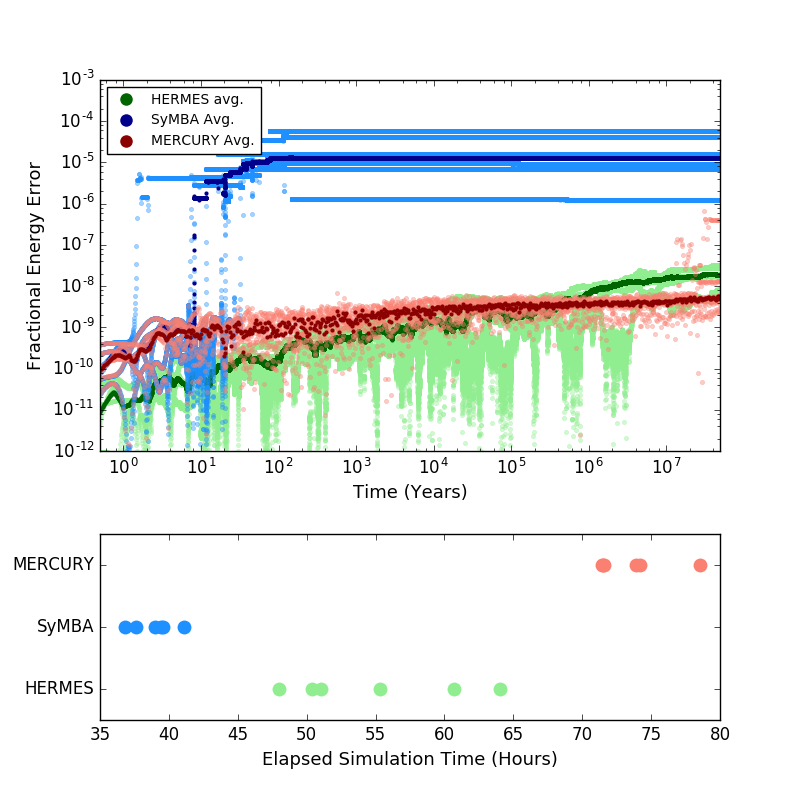
\includegraphics[scale=0.45]{chap4/images/energy_avg_FULL.png}}
\caption{A test of \hermes, \mercury and \symba for collections of 50Myr, 50 planetesimal runs. 
Top panel shows the relative energy error over time, with individual runs in lighter shades and averaged values in dark shades.
Bottom panel shows the elapsed simulation times of individual runs, using the same colour scheme as the top panel.
 }
\label{fig:Np100test}
\end{figure}

Looking at the top panel, \symba incurs significant energy jumps early in the simulation. 
We suspect these energy jumps are due to inadequately resolved close encounters, since the energy jumps are uncorrelated with particle collisions. 
We simulated runs using different combinations of {\sc \tt RHSCALE} and {\sc \tt RSHELL}, i.e. the parameters which define close encounter regions, but were unable to resolve these energy jumps. 
By the end of the simulation, \symba is orders of magnitude less accurate than \mercury and \hermes.

We see that \hermes initially has the lowest energy error, but grows faster than \mercury.  
The final energy error for an integration therefore depends on the particular problem (length of simulation, timestep, number and severity of close encounters etc.).
Furthermore, we find that some \mercury simulations undergo significant energy jumps, probably also due to very close encounters that are not properly resolved. 
Our adaptive $\HSF$ algorithm (Section~\ref{sec:HSFop}) protects against these situations from occurring, and for a properly chosen $\HSF$ and $dt$ combination we find the energy growth of \hermes to be well behaved. 

The bottom panel shows that for these simulations \hermes is slower than \symba but faster than \mercury. 
We see that \hermes exhibits a larger variance in elapsed simulation times than \mercury and \symba. 
This is because when the adaptive $\HSF$ routine is engaged, $\HSF$ can be enlarged considerably during severe encounters, slowing down the integrator. 
In summary, these simulations show that \hermes provides a good balance between speed and accuracy.

\section{Conclusion}
\label{sec:Conclusion}
In this Chapter we have presented \hermes, a hybrid integrator capable of integrating close encounters and collisions. 
\hermes integrator is composed of two parts, a global simulation which contains all particles and a mini simulation which contains all active particles (e.g. stars and planets) plus any semi-active/test particles (e.g., planetesimals) involved in a close encounter.
The global simulation is integrated with \whfast while the mini simulation is integrated with \ias.
Comparing \hermes to the openly available \mercury and \symba we find that \hermes provides a good balance between accuracy and speed.

\hermes takes a more direct approach when integrating close encounters over other methods.
However this has enabled us to characterize the error of \hermes, and we find that the switching error from a single close encounter is well described by Eq.~\ref{eq:Escheme}, which we calculate from first principles.
The total energy error of \hermes for an $N$-body simulation is well described by a random walk, (see Eq.~\ref{eq:Etot}) with the step size being the switching error.

We have also developed an adaptive algorithm that chooses the optimal Hill switch factor, $\HSF$, which governs the size of the close encounter region surrounding each particle.
This frees the user from optimizing integrator parameters for typical cases. 
Finally, we have introduced a number of new features in \reb, including a new heliocentric version of \whfast, semi-active particles (see Fig.~\ref{fig:bodies}) and inelastic collisions.

We have showcased a number of problems well-suited for \hermes, and compared our integrator's performance to similar integrators in the literature. 
In particular, we integrated the outer Solar System with planetary masses increased by a factor of 50, and we simulated a planet migrating through a disk of planetesimals, both in the limit of many planetesimals ($\sim 10^5$) and short times ($\sim 10^3$ orbits), and few planetesimals (100) and long times ($\sim 10^8$ orbits).
Many more types of problems are possible with \hermes, and additional examples can be found at {\sc \tt https://github.com/hannorein/rebound}.

\chapter[Stability of Planetary Systems]{A Machine Learns to Predict the Stability of Tightly Packed Planetary Systems}
\label{chap:Stability}

\section{Chapter Overview}

The requirement that planetary systems be dynamically stable is often used to vet new discoveries or set limits on unconstrained masses or orbital elements. 
This is typically carried out via computationally expensive N-body simulations.
We show that characterizing the complicated and multi-dimensional stability boundary of tightly packed systems is amenable to machine learning methods. 
We find that training a state-of-the-art machine learning algorithm on physically motivated features yields an accurate classifier of stability in packed systems. 
On the stability timescale investigated ($10^7$ orbits), it is 3 orders of magnitude faster than direct N-body simulations. 
Optimized machine learning classifiers for dynamical stability may thus prove useful across the discipline, e.g., to characterize the exoplanet sample discovered by the upcoming Transiting Exoplanet Survey Satellite (TESS).

\section{Introduction}
In order to characterize planetary systems, it is common practice to assume long-term stability in order to set upper limits on planetary masses and orbital eccentricities \citep[e.g.][]{Lissauer2011, Steffen2013, Tamayo14b, Tamayo2015}.
This involves running grids of direct N-body integrations over the large multi-dimensional parameter space of initial conditions that are consistent with observational error.
In practice, however, one can often explore only a minute fraction of the phase space; in the case of many systems discovered by the Kepler mission, each integration requires several weeks of computation to simulate timescales comparable to the star's age ($\gtrsim 10^{11}$ planetary orbits) with current hardware.
An efficient classifier of dynamical stability would thus be invaluable.

In this investigation, we specialize to the case of tightly packed systems, where the interplanetary separations are less than 10 mutual Hill radii ($R_H$), where
\begin{equation}
R_H \equiv \left(\frac{M_1+M_2}{3M_\star} \right)^{1/3} a_1,
\end{equation}
$M_1, M_2$ and $M_\star$ are the masses of a pair of planets and the central star, and $a_1$ is the semimajor axis of the inner planet.
This regime has long been recognized as important in the early stages of planetary systems when bodies are still merging, and has received much attention.

For the special case of two-planet systems, one can prove that there exists a bifurcation in the dynamics that forbids planets from undergoing close encounters for all time \citep{Marchal82, Milani83}.
In the case of co-planar, circular orbits, the transition occurs at a planetary separation of 3.46 $R_H$ \citep{Gladman1993}.
If the planets are more widely separated than this threshold, the system is Hill stable, i.e., close encounters are forbidden for all time.
While there are ways for planets to escape or collide with the star without undergoing close encounters \citep[e.g.,][]{Deck12, Veras13hill}, and eccentric planets that fail this criterion can nevertheless be long-lived \citep[e.g.,][]{Gladman1993}, the Hill criterion provides good guidance, particularly in the low-eccentricity regime \citep{Barnes06}.

In the general case with more than two planets, however, the additional degrees of freedom preclude a topological criterion for Hill stability.
This has led many authors to perform suites of N-body simulations and fit empirical curves to the results.
Because of the prohibitively large phase space of possible initial conditions, several authors \citep[][Obertas et al., submitted]{Chambers1996, Faber07, Smith09} have considered the special case of initially circular, planar orbits with all planet pairs having equal Hill separations $\Delta$, defined as the difference in semimajor axis divided by $R_H$.
They find that even in cases where each pair of planets satisfies the Hill criterion, the system nevertheless destabilizes, and that the associated timescale seems to grow exponentially with Hill separation.
However, the fitted coefficients vary as the number of planets and planetary masses are varied, and introducing inclinations \citep{Marzari02}, eccentricities \citep{Ito99, Chatterjee08, Pu2015}, or unequal spacings between planets \citep{Marzari14} change the instability timescales substantially.
For a given planetary system, it is therefore not always clear which scaling law is appropriate to apply, and what confidence one can have in the resulting estimate.

For this investigation we take a machine learning approach.
High dimensional classification tasks are ubiquitous across industry and data science, and sophisticated machine learning algorithms have been developed to tackle these problems.
Such techniques have been highly successful in an astronomical context for several image classification tasks, e.g., assigning morphological types to galaxies \citep{Collister04}; however, they have seen little use in dynamical classification to date\citep[see][for a recent counterexample]{Petrovich15}.
 
\section{Methods}
We choose to frame the problem as a binary classification task, i.e., predicting whether or not a given planetary system is stable (over a given timescale).
Each ``example" (planetary system) is described by a set of ``features" that the algorithm uses to predict stability, in the form of a probability between 0 and 1.
In supervised machine learning, an algorithm is first trained on examples where it is told the correct answer (stable or not stable).
The trained algorithm can then be used to predict on new examples.

\subsection{Dataset} \label{dataset}
In order to train our algorithms, we generated a dataset of 5000 N-body integrations of 3-planet systems over $10^7$ orbits of the innermost body.
We focus on 3-planet systems since there exists an analytic criterion for the case of two planets, and systems with more planets exhibit qualitatively similar behavior.
The number of simulations and length of integration were chosen to generate a dataset at limited computational cost, and assess the value of investing significant computing time to train classifiers on astrophysically relevant timescales of $\sim 10^9$ orbits.
Because we expect that instability timescales of $10^7$ and $10^9$ orbits are both physically driven by Chirikov diffusion due to the overlap of mean-motion resonances (see Fig.\:2 in Obertas et al., submitted), we expect the performance of models trained on this dataset to be comparable to that of similar algorithms trained on longer datasets.

With a view toward applying these models to Kepler discoveries, we adopted a solar-mass star, 5 $M_\Earth$ (Earth-mass) planets, and drew the innermost planet's semimajor axis randomly between 0.04 and 0.06 AU.
We note, however, that our results are strictly scale-free, and can be applied to comparable systems with masses, orbital periods and semimajor axes expressed in terms of the star's mass, innermost planet's orbital period and semimajor axis, respectively.
The second planet's semimajor axis was separated from the first by a number of mutual Hill radii drawn from a uniform distribution in the range $[5,9]$.  
The third planet's separation was then independently drawn from the same distribution, yielding unevenly spaced planets.
The particular range of Hill-radius separations was chosen to capture the regime of interest on our adopted timescale of $10^7$ orbits and roughly generate a balanced dataset of stable and unstable systems (this yielded 1479 stable systems out of 5000).
Eccentricities and inclinations were drawn independently for each planet from uniform distributions over [0, 0.02] and [0, 1$^\circ$], and the remaining angles were drawn randomly over [0,$2\pi$].

All integrations were performed using the {\sc \tt WHFAST} integrator \citep{Rein2015b} in the open-source {\sc \tt REBOUND} N-body package \citep{Rein2012}, which is written in \texttt{C99} and comes with an optional \texttt{python} interface.
We adopted a timestep of 1\% of the innermost planet's orbital period, and classified systems as unstable if any pair of planets came within 1 Hill radius of each other during the simulation.

\subsection{Metrics} \label{metrics}
Binary classifiers are often evaluated on their {\it precision} (here the fraction of systems that are actually stable when the model predicts stability) and {\it recall} (the fraction of systems the model predicts are stable out of the truly stable cases).  
For typical algorithms that predict probabilities of class membership, one can trade off between precision and recall by varying the threshold probability for classification.
For example, a conservative model that only classifies systems as stable if it predicts a probability of stability greater than 0.99 will be right most of the times that it predicts stability (high precision), but will miss all the stable systems that were assigned slightly lower probabilities (low recall).
The appropriate threshold depends on the application (e.g., if predicting DNA matches for crime cases, one might set a high threshold as above to have confidence in predicted matches).

When comparing two models, one can plot pairs of precision and recall scores for all possible thresholds to generate a precision-recall curve.
A common scalar metric for comparing classifiers is the area under this curve (AUC), which would be unity for a perfect model.

\subsection{Algorithm Training} \label{training}
After experimenting with several machine learning algorithms (random forest and support-vector machine implementations in the {\tt Python scikit-learn} library), we found that gradient-boosted decision trees (GBDT\footnote{GBDT algorithms create and combine large numbers of individually weak but complementary classifiers to yield a robust estimator \citep{Friedman01}}) {\tt XGBoost v0.6} \citep{Chen16} gave the best results for our dataset.

A recurring theme in machine learning is that of ``overfitting," an algorithm's tendency to latch onto irrelevant idiosyncrasies in the training set that cause it to predict poorly on unseen examples.
Different algorithms therefore try to penalize overly complicated models in an effort to retain only the broad features that are likely to generalize well.
In practice, the user navigates this balance between simplicity and complexity empirically, by tuning an algorithm's ``hyperparameters" that mediate this tradeoff, training it, and checking performance (Sec.\:\ref{metrics}) on unseen data; this process, together with trying different features to maximize performance, is known as cross-validation. 
In order to rule out the possibility of (sometimes subtle) mistakes in cross-validation yielding overly optimistic performance metrics, it can be good practice to assign a subset of the data to a holdout (test) set that is never seen by the algorithm during cross-validation.
Evaluation of the final model on the holdout set therefore provides robust metrics of the trained algorithm's expected performance on unseen examples; consistency between the cross-validation and test scores also suggest a robust cross-validation methodology.
In our case, we randomly assigned 1500 systems to a holdout test set, and used only the remaining 3500 for cross-validation.

A typical technique to reduce statistical fluctuations when comparing the performance of different sets of hyperparameters is $k$-fold cross validation.
One begins by splitting the training examples into $k$ evenly sized groups; then, for each group, one trains the model on the remaining $k-1$ chunks, and uses the remaining group to evaluate performance.
The scores from the $k$ folds are then averaged, reducing the variance in the estimate.
Finally, it is generally good practice to use stratified cross-validation, whereby one ensures that each of the $k$ folds is assigned an approximately equal number of samples from each class (stable and unstable).

{\tt XGBoost} has several hyperparameters, so we sequentially performed grid searches through 2-dimensional cuts through the parameter space, evaluating performance through the precision-recall AUC (Sec.\:\ref{metrics}) using stratified, 5-fold cross-validation on the training set of 3500 examples.
Values of the final adopted hyperparameters for the algorithm are discussed in Sec.\:\ref{IC} and \ref{shortintegrations} can be found in Table \ref{hyper}.

\begin{table}[h]
\begin{center}
\caption{Hyperparameters used for the initial-conditions (IC) model (Sec.\:\ref{IC}) and short-integrations (SI) model (Sec.\:\ref{shortintegrations}), and their associated performance. \label{hyper}}
\begin{tabular}{ c|c|c}
 	& IC Model & SI Model \\
  \hline \hline			

  {\tt base\_score} & 0.5 & 0.5\\
  {\tt colsample\_bylevel} & 1 & 1\\
  {\tt colsample\_bytree} & 1 & 1\\
  {\tt gamma} & 0 & 0\\
  {\tt learning\_rate} & 0.001 & 0.00359 \\
  {\tt max\_delta\_step} & 0 & 0 \\
  {\tt max\_depth} & 6 & 8 \\
  {\tt min\_child\_weight} & 1.0 & 1.2 \\
  {\tt missing} & None & None \\
  {\tt n\_estimators} & 5000 & 5000 \\
  {\tt objective} & binary:logistic & binary:logistic\\
  {\tt reg\_alpha} & 0 & 0 \\
  {\tt reg\_lambda} & 1 & 1 \\
  {\tt scale\_pos\_weight} & 1 & 1\\
  {\tt seed} & 27 & 27 \\
  {\tt subsample} & 0.4 & 0.5\\
  \hline \hline
  AUC (Cross-Validation) & 0.842 $\pm$ 0.012 & 0.911 $\pm$ 0.012\\
  AUC(Test Dataset) & 0.843 & 0.898 \\
  Recall (At 90\% Precision) & 0.52 & 0.68\\
    \hline  
\end{tabular}
\end{center}
\end{table}

\section{Results} \label{results}
\subsection{Model 1: Learning from Initial conditions} \label{IC}
We begin by considering as features the initial orbital elements and orbital period of each planet, and the interplanetary separations between adjacent planets in units of mutual Hill radii. 
We then trained an {\tt XGBoost} classifier on these features (Section~\ref{training}), allowing us to predict the stability of each system in the test set in the form of an estimated probability. 

As discussed in Section~\ref{model}, a threshold probability is required for classifying a system as stable/unstable, and is a subjective choice that depends on the desired qualities of the classifier.
For our purposes we argue it is logical to adopt a conservative threshold, in the sense that if the model predicts stability, there is a strong likelihood that the system is actually stable (high precision).
This follows from the fact that it is computationally much faster to verify that a system is unstable (on short timescales) than it is to check that it is stable (on long timescales).
We choose to require a precision of $90\%$ on our test dataset, which corresponded to the model only classifying systems as stable if their predicted stability probability is larger than a 0.785 threshold.

Since previous works have identified the Hill separations between adjacent planets as important features \citep{Chambers1996, Marzari14}, we plot the performance of the model projected onto this 2D plane (Fig.\:\ref{ariplot}).

\begin{figure}
 \centering \resizebox{0.99\columnwidth}{!}{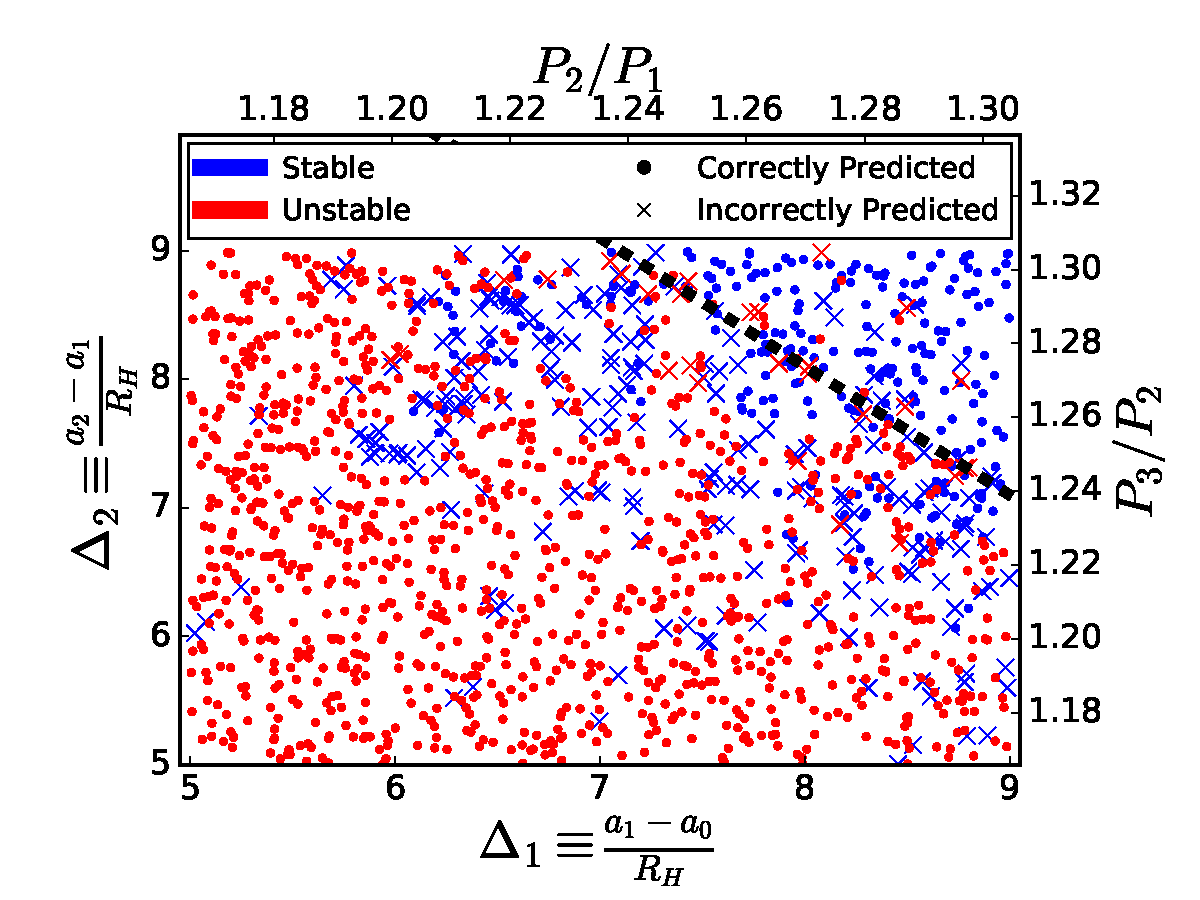
\includegraphics{chap5/figures/ICpredictions}}
 \caption{
     Performance on the test dataset using the machine learning model trained on system's initial conditions.
     Stable systems are marked blue, unstable systems are marked red.  
     Correctly classified systems are plotted as circles, incorrect predictions are marked as crosses.
     The bottom and left axes show Hill-sphere separations $\Delta$ for the inner and outer planet pairs, respectively.
     The top and right axes correspond to period ratios between the planet pairs.
     The dashed black line corresponds to the Lissauer-family model $\Delta_1 + \Delta_2 > 16.1$.    
    \label{ariplot}}
\end{figure}

Looking at the dashed, black line in Figure~\ref{ariplot}, one can see that to first order, the model's prediction boundary roughly obeys the relation $\Delta_1 + \Delta_2 > 16.1$.
This is in fact the form of the simple criterion suggested by \cite{Lissauer2011}, who quote $\Delta_1 + \Delta_2 > 18$ for stability on timescales of $10^9$ orbits. 
Because we consider stability on shorter timescales, the threshold number of Hill radii should be adjusted for a fair comparison.
We term models of the form $\Delta_1 + \Delta_2 > x$ ``Lissauer-family" models, and find 16.1 is the threshold for Lissauer-family models that yields a precision of 90\% on this dataset.

As stated above, a conservative probability threshold has the disadvantage that the model will misclassify many stable systems as unstable (low recall).  
This is easily seen by considering different Lissauer-family models (dashed black line in Fig.\:\ref{ariplot}), i.e. imposing different threshold values than 16.1 and generating lines parallel to the one plotted.
Larger threshold values ensure that a larger fraction of the systems to the right of the boundary (i.e., those predicted stable) are in fact stable (blue), leading to higher precision.
However, this lowers the recall, since now fewer of the stable systems (blue) are predicted to be stable by the model (i.e., lie to the right of the line).
For a fixed precision of 90\%, the machine learning model has a significantly higher recall ($52\%$) than the Lissauer-family model ($30\%$). 
This is because the machine learning model can use information in the features not visible in this 2D projection to make better predictions.


\subsection{Model 2: Generating Features from Short Integrations} \label{shortintegrations}

An important factor determining the performance of a machine learning algorithm is the quality of the features it is provided for each of the training examples.
To this end, we improved upon the previous model (Section~\ref{IC}) by generating new features from short N-body integrations.
To create the new features, we performed simulations over $10^4$ orbits (0.1\% of the instability timescale probed) for each of the 5000 systems in the dataset, and recorded each planet's orbital elements and the current Lyapunov timescale every 5 orbits.

Because we suspect that the instability is driven by overlapping mean-motion resonances, we first generated features that capture the variation in semimajor axes, which would vanish if the dynamics were purely secular \citep{SSD1999}.  
In particular, we generated features for the standard deviation and maximum value of each planet's semimajor axis over the $10^4$ orbits , normalized to the mean value over the same period  ({\tt std\_ai} and {\tt max\_ai}, where {\tt i} denotes the planet number) .  
In addition, we generated features for the same quantities over only the first 50 orbital periods in order to capture the variations on orbital timescales ({\tt std\_window\_ai} and {\tt max\_window\_ai}).
Furthermore, we noticed in early attempts that some misclassified systems exhibited drifts in semimajor axis, so we generated slope features from linear fits to each of the three planets' semimajor axes, normalized to the mean semimajor axis divided by the integration time ({\tt slope\_ai}).
For the eccentricities of each planet, we generated features for the mean, standard deviation, maximum and minimum values over the full $10^4$ orbits, and normalized them to the eccentricity that planet would require to reach its nearest neighbor's semimajor axis ({\tt avg\_ei}, {\tt std\_ei}, {\tt max\_ei}, {\tt min\_ei}).
For the Lyapunov time we generated a single feature corresponding to the value measured at the end of the integration, normalized to the innermost orbital period.
Finally, we added features for the two pairs of initial Hill-radius separations, and for the minimum and maximum initial Hill-radius separations.
We experimented with adding features involving the planetary inclinations, but they did not significantly improve the models.

A summary of all the features used can be found in Table \ref{features}, which are ordered by their importance.
We quantify the importances through the {\tt Gain} value recorded by {\tt XGBoost}, which corresponds to the gain in accuracy that a given feature provides when it is introduced into the underlying decision trees used by {\tt XGBoost}.  
The units are normalized so that the gains sum to 100.
We find that the variations in the middle planet's semimajor axis are the most informative in this sense.
We interpret this as suggesting that the instabilities in these closely packed systems are driven by the overlap of mean motion resonances (which change the semimajor axes), rather than secular effects (which would keep the semimajor axes constant).

\begin{table}[h]
\begin{center}
\caption{`Short-Integration' Model Feature Importances. See text for a description of the gain and of the features. \label{features}}
\begin{tabular}{ c|c }
Feature & Gain \\
  \hline \hline			
  {\tt max\_a2} & 20.3 \\
  {\tt std\_a2} & 8.3 \\
  {\tt mindaOverRH} & 2.6 \\
  {\tt maxdaOverRH} & 2.6 \\
  {\tt std\_a3} & 2.3 \\
  {\tt max\_e2} & 2.3 \\
  26 more features... & \\
  \hline  
\end{tabular}
\end{center}
\end{table}

Finally, we compare the performance of this `short-integration' model to the previous `initial-condition' model.
Fig.\:\ref{dianaplot} shows that while both models often assign unstable systems (blue bins) a low predicted probability, the `initial-condition' model assigns stable systems (green bins) a wide range of predicted probabilities, translating to a lower recall.
In contrast, the `short-integration' model more confidently assigns high predicted probabilities to stable systems, better separating the two classes.
Again setting the predicted probability threshold so as to obtain 90\% precision, the recall improves to 68\%.

\begin{figure}
 \centering \resizebox{0.99\columnwidth}{!}{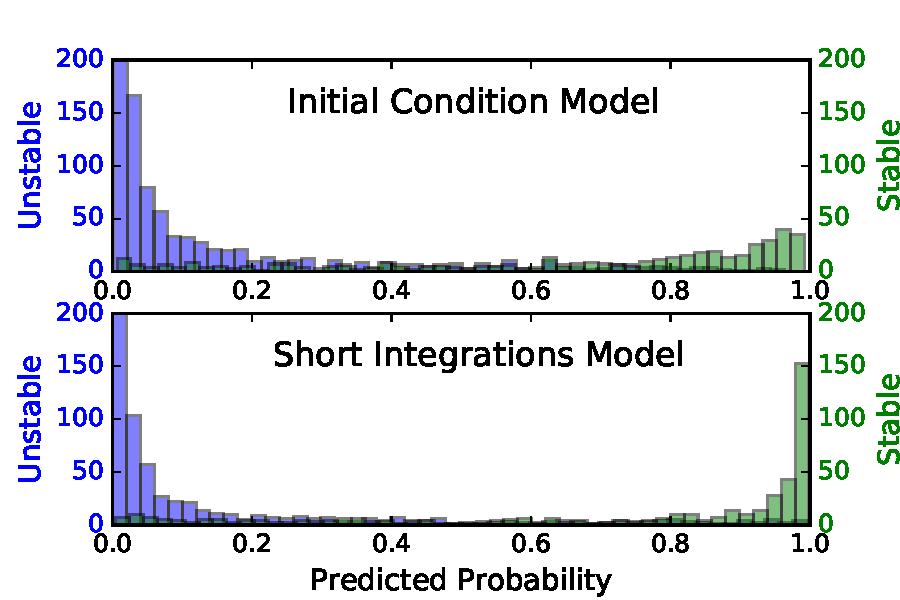
\includegraphics{chap5/figures/histograms}}
 \caption{
     Comparison of predictions of the initial-condition and short-integration models on the test set.
     Stable systems are shown in green, unstable systems are shown in blue, and the model-predicted probability of stability for each system is shown along the x-axis.
     The leftmost blue bin is cut off to render smaller bins visible--in the top panel it reaches 395, and in the bottom panel 640.
    \label{dianaplot}}
\end{figure}

\section{Discussion \& Conclusion} \label{conclusion}
In this investigation, we numerically integrated a dataset of 5000 three-planet systems over $10^7$ orbits.
We then trained machine learning algorithms to classify systems' orbital stability on this timescale.
In particular, we trained two models using the gradient-boosted decision trees algorithm {\tt XGBoost}, an `initial-conditions' model (Sec.\:\ref{IC}) that learned only from the system's initial orbital elements, and a `short-integration' model (Sec.\:\ref{shortintegrations}) that generated features from short N-body integrations.
We then compared their performance to `Lissauer-family models' that require the sum of the interplanetary separations (expressed in mutual Hill radii) to be greater than a particular threshold.

We summarize the investigated models' performances in Fig.\:\ref{prcurves}, which plot values for the respective classifier's precision and recall for all possible values of the probability threshold above which the model labels a system as stable.
As discussed above, the appropriate choice of this threshold depends on the desired qualities of the classifier.
Above we advocated for conservative models that are correct 90\% of the time when a system is predicted stable (90\% precision), but different applications might consider different criteria.

\begin{figure}
 \centering \resizebox{0.99\columnwidth}{!}{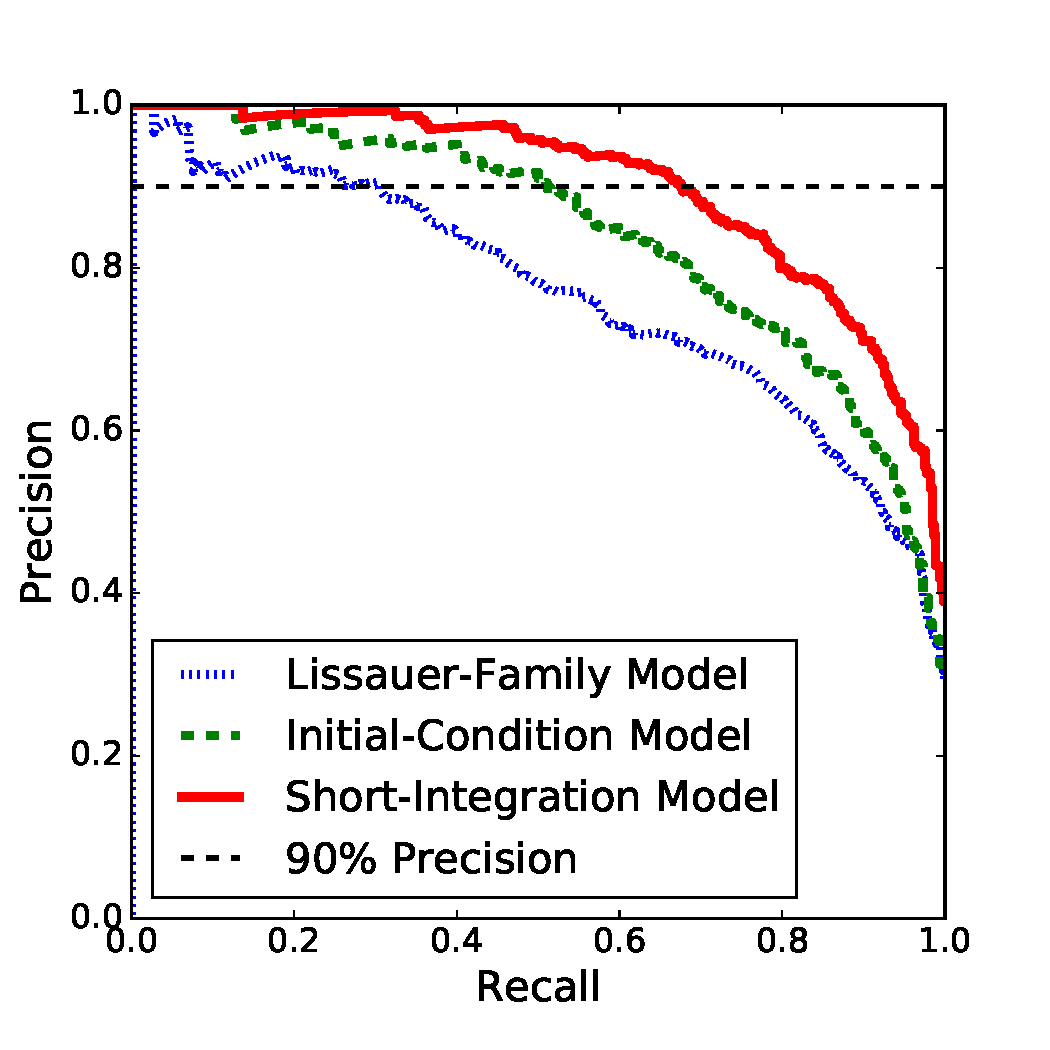
\includegraphics{chap5/figures/prcurves}}
 \caption{
     Precision-recall curves for each model in this Chapter, generated from all possible values of the model's threshold classification probability.
     The Lissauer-family models predict stability if the sum of the Hill-sphere separations is greater than a particular threshold, and the corresponding curve was generated by considering all possible threshold values.
     The horizontal black-dashed line is the 90\% precision requirement we imposed on all models in this Chapter. 
    \label{prcurves}}
\end{figure}

By generating dynamically relevant features from short integrations, our best machine-learning model:
\begin{itemize}
	\item Dominates other models at all threshold values.
	\item Recovers 2.25 as many of the truly stable systems (has 2.25 times higher recall) as a Lissauer-family model at a fixed precision of 90\%.
	\item Is three orders of magnitude faster than direct N-body integration. Performing the short integration, generating the features and evaluating the model for a given system takes $\sim$ 1 second with current technology.
\end{itemize}

An important limitation of this work are the fixed masses (5 Earth masses around a solar-mass star) and the comparatively short integration timescales ($10^7$ orbits).
Our results strongly motivate investing computational time to generate datasets over longer timescales with a range in masses.
Running these integrations in a reproducible and openly accessible manner (Rein \& Tamayo, in prep.) would allow this dataset to be used as a standard on which current and future models could be evaluated and compared, and as a database of integrations to test theoretical investigations.  

Such classifiers could be used in many of the ways that direct N-body integrations currently are employed, but these models' dramatically improved efficiency would allow much faster and complete explorations of parameter space, e.g.:
\begin{itemize}
	\item Mapping out the stability boundary in mass-eccentricity space for observed transiting systems.
	\item Mapping out the parameter space that unseen planets could stably inhabit in a given system to guide observational follow-up strategies or theoretical considerations.
	\item Vetting low signal-to-noise detections through stability constraints.
	\item Generating stable or unstable systems for theoretical population studies.
	\item As a stopping condition for simulations once they achieve a dynamically long-lived configuration.
\end{itemize}

Such tools may be of particular interest for the upcoming Transiting Exoplanet Survey Satellite (TESS).
While transit-timing variations (TTVs) have been powerful tools for constraining the masses and eccentricities of near-resonant Kepler systems \citep[e.g.,][]{Ford12, Steffen2013, Deck15}, TESS' shorter time baselines and planets' smaller semimajor axes will render such analyses difficult or impossible.
It is therefore likely that in many systems, stability considerations will provide the strongest constraints on planetary masses and eccentricities, and this will be important for guiding the substantial radial-velocity follow-up efforts from the ground. 

More broadly, we have shown that machine learning can be a powerful tool for high-dimensional classification problems in dynamics and other fields.
But in addition to their predictive power, our models also revealed new insights into the underlying dynamics.
In particular, the most informative features in our model based on short integrations were the variations in the middle planet's semimajor axis.
This suggests that the orbital instabilities are driven by the overlap of mean motion resonances (which vary the semimajor axes) rather than the secular chaos at work in our own solar system \citep{Lithwick11secularchaos, Batygin15}, which proceeds with constant semimajor axes.

\chapter[Analysis of HD155358]{Resonant structure, formation and stability of the planetary system HD155358}
\label{chap:HD155358}

\section{Chapter Overview}

Two Jovian-sized planets are orbiting the star HD155358 near exact mean motion resonance (MMR) commensurability. 
In this work we re-analyze the radial velocity~(RV) data previously collected by \citet{Robertson2012}.
Using a Bayesian framework we construct two models -- one that includes and one that excludes gravitational planet-planet interactions (PPI).
We find that the orbital parameters from our PPI and noPPI models differ by up to $2\sigma$, with our noPPI model being statistically consistent with previous results.
In addition, our new PPI model strongly favours the planets being in MMR while our noPPI model strongly disfavours MMR.
We conduct a stability analysis by drawing samples from our PPI model's posterior distribution and simulating them for $10^9$ years, finding that our best-fit values land firmly in a stable region of parameter space.

We explore a series of formation models that migrate the planets into their observed MMR.
We then use these models to directly fit to the observed RV data, where each model is uniquely parameterized by only three constants describing its migration history.
Using a Bayesian framework we find that a number of migration models fit the RV data surprisingly well, with some migration parameters being ruled out.

Our analysis shows that planet-planet interactions are important to take into account when modelling observations of multi-planetary systems.
The additional information that one can gain from interacting models can help constrain planet migration parameters.

\section{Introduction}
\label{sec:intro}
The past decade has marked an explosion in the number of discovered multi-planet systems, with almost 600 known to date \citep{NASAEA}. 
Jovian planets have been detected in these exoplanetary systems, and the range of conditions under which they can form is uncertain.
For example, many Jovian planets are observed inside the snowline of their host star \citep[e.g.][]{Hayashi1981}, and it is unclear whether they formed in-situ \citep{Boley2016, Huang2016, Batygin2016} or beyond the snowline and migrated in afterwards \citep{Mayor1995, Lin1996, Pollack1996}.
For systems near mean motion resonance (MMR), planetary migration offers a natural formation mechanism \citep[e.g.][]{Lee2002, Rein2009}.
Since roughly $30\%$ of Jovian-sized planets with a detected planet companion are near a first-order MMR \citep{NASAEA}, at least a substantial fraction of planetary systems are likely to have formed via migration. 

The star HD155358 hosts two observed Jovian-sized planets orbiting inside the snowline near a MMR. 
The star has a mass of $0.92~M_{\odot}$, and the planets have orbital periods $P_1 = 194$ and $P_2 = 392$~days, respectively, about 2\% away from the exact 2:1 commensurability \citep[][hereafter \R]{Robertson2012}. 
In addition, HD155358 is also among the lowest metallicity stars known to host Jovian-sized planets \citep{Cochran2007}.
Since the presence of MMR can provide additional constraints on formation and evolution, HD155358 provides an opportunity to better understand the formation of Jovian planets in exoplanetary systems.

The HD155358 system has been previously studied by many scientists \citep{Cochran2007,Fuhrmann2008,Robertson2012,Andre2016}.
Of particular interest is the work by \R, who updated the orbital parameters initially reported by \citet{Cochran2007} after collecting additional radial velocity (RV) observations.
In \R the orbital properties were derived from \textsc{GaussFit\-} \citep{Jefferys1988} and \textsc{SYSTEMIC} \citep{Meschiari2009}, and planet-planet interactions were not included in their analysis (Robertson 2016, private communication). 
For well-separated orbits this assumption is valid and simplifies the analysis.
However, near a MMR this approximation can lead to different orbital solutions and therefore different formation constraints and evolutionary predictions. 
In particular, without planet-planet interactions one cannot draw any conclusion as to whether the system is in resonance or not. 

In this work we re-analyze HD155358 using the RV observations collected by \R.
In Sect.~\ref{sec:orb}, we derive new orbital parameters using a Bayesian framework coupled to direct N-body integrations and assess the probability that the system is in resonance.
In Sect.~\ref{sec:form}, we perform simulations constraining the migration history, and in Sect.~\ref{sec:stability} conduct a stability analysis. 
We conclude with a discussion in Sect.~\ref{sec:conc}.

%%%%%%%%%%%%%%%%%%%%%%%%%%%%%%%%%%%%%%%%%%%%%%%%%%%
%%%%%%%%%%%%%%%%%%%%%%%%%%%%%%%%%%%%%%%%%%%%%%%%%%%
\section{Best-Fit Parameters and Resonance Analysis}
\label{sec:orb}
\subsection{Methods}
\label{sec:Fit}
The RV data used for this analysis comes from Table 2 of \R. 
We model this system using \reb \citep{Rein2012}, an open-source N-body code for simulating problems in planetary dynamics.
Using \reb we can extract the motion of the central star over the course of our simulation, comparing it directly to the RV data. 

In this work we explore two different models -- one that includes the planet-planet gravitational interactions, abbreviated as PPI model, and one that excludes planet-planet gravitational interactions, abbreviated as noPPI model. 
This is achieved in \reb by initializing each planet as either a massive body (PPI model) or a semi-active particle (noPPI model).
Semi-active particles can gravitationally interact with massive bodies (e.g. the central star), but cannot interact with other semi-active particles. 
For reference, \R does not include the gravitational interactions between the planets, and is analogous to our noPPI model.  

We construct our models using a Bayesian framework, where the quantity of interest is the posterior probability density function. 
Benefits of conducting an analysis within a Bayesian framework include marginalization over nuisance parameters, preservation of correlations between parameters, and a natural Occam's razor when comparing models \citep[see e.g.][for a full discussion]{Gregory2005}.
Using Bayes' theorem we calculate the (unnormalized) posterior probability according to:
\begin{equation*}
p(\theta | D) \propto p(D | \theta) p(\theta),
\label{eq:Bayes}
\end{equation*}
where $\theta$ are the parameters in our model, $D$ is our data, $p(\theta)$ is our prior probability on $\theta$, $p(D | \theta)$ is the probability of $D$ given $\theta$ (i.e. the likelihood function), and $p(\theta | D)$ is our posterior probability.
As with most models that employ Bayes' theorem, the posterior probability cannot be analytically computed, requiring the use of numerical methods for approximating it. 
We use \emcee, an open-source affine-invariant Markov chain Monte Carlo (MCMC) routine  \citep{Foreman-Mackey2013}.  

For our models we assume that the system is co-planar, and use the known value of stellar mass, $m_* = 0.92M_{\odot}$.
For each planet we have the following parameters: the reduced mass, $m\sin(i)$, the semi-major axis, $a$, the eccentricity, $e$, the argument of periapsis, $\omega$, and the mean anomaly $M$. 
To avoid singularities for $\omega$ (which is ill-defined when $e\sim0$), we fit $h=e\sin(\omega)$ and $k=e\cos(\omega)$ instead of $e$ and $\omega$.
We also add an offset parameter $\gamma$ to account for any stellar drift along the line of sight, a jitter parameter $J$ to account for any stellar noise and unreported instrument variability, and a viewing angle parameter sin$(i)$.
This yields a total of 13 parameters to be sampled by the MCMC. 

We initialize our MCMC chain with values similar to the best fit values of \R to speed up convergence, and use the following priors on our parameters: $0.4M_J<m_1\textrm{sin}(i) < 2M_J$, $0.4M_J<m_2\textrm{sin}(i) < 2M_J$, $0.2 \textrm{AU}<a_1< 0.8\textrm{AU}$, $0.8\textrm{AU}<a_2< 1.4\textrm{AU}$, $1<h_1, h_2, k_1, k_2<-1$, $0<\omega_1, \omega_2, M_1, M_2<2\pi$, $-40\textrm{m/s}<\gamma<40\textrm{m/s}$, and $0\textrm{m/s}<J^2<50\textrm{m/s}$.
Our MCMC chain consists of an initial burnin phase of 1000 steps with 400 walkers, after which the MCMC walkers are resampled near the best solution and run for 5000 steps.
In \reb we use the \whfast integrator \citep{Rein2015b} with a timestep of $P_1/200$, leading to a bounded relative energy error of $<10^{-7}$.

%%%%%%%%%%%%%%%%%%%%%%%%%%%%%%%%%%%%%%%%%%%%%%%%%%%

\subsection{Best Fit Parameters}
\label{sec:Results}
\begin{figure*}
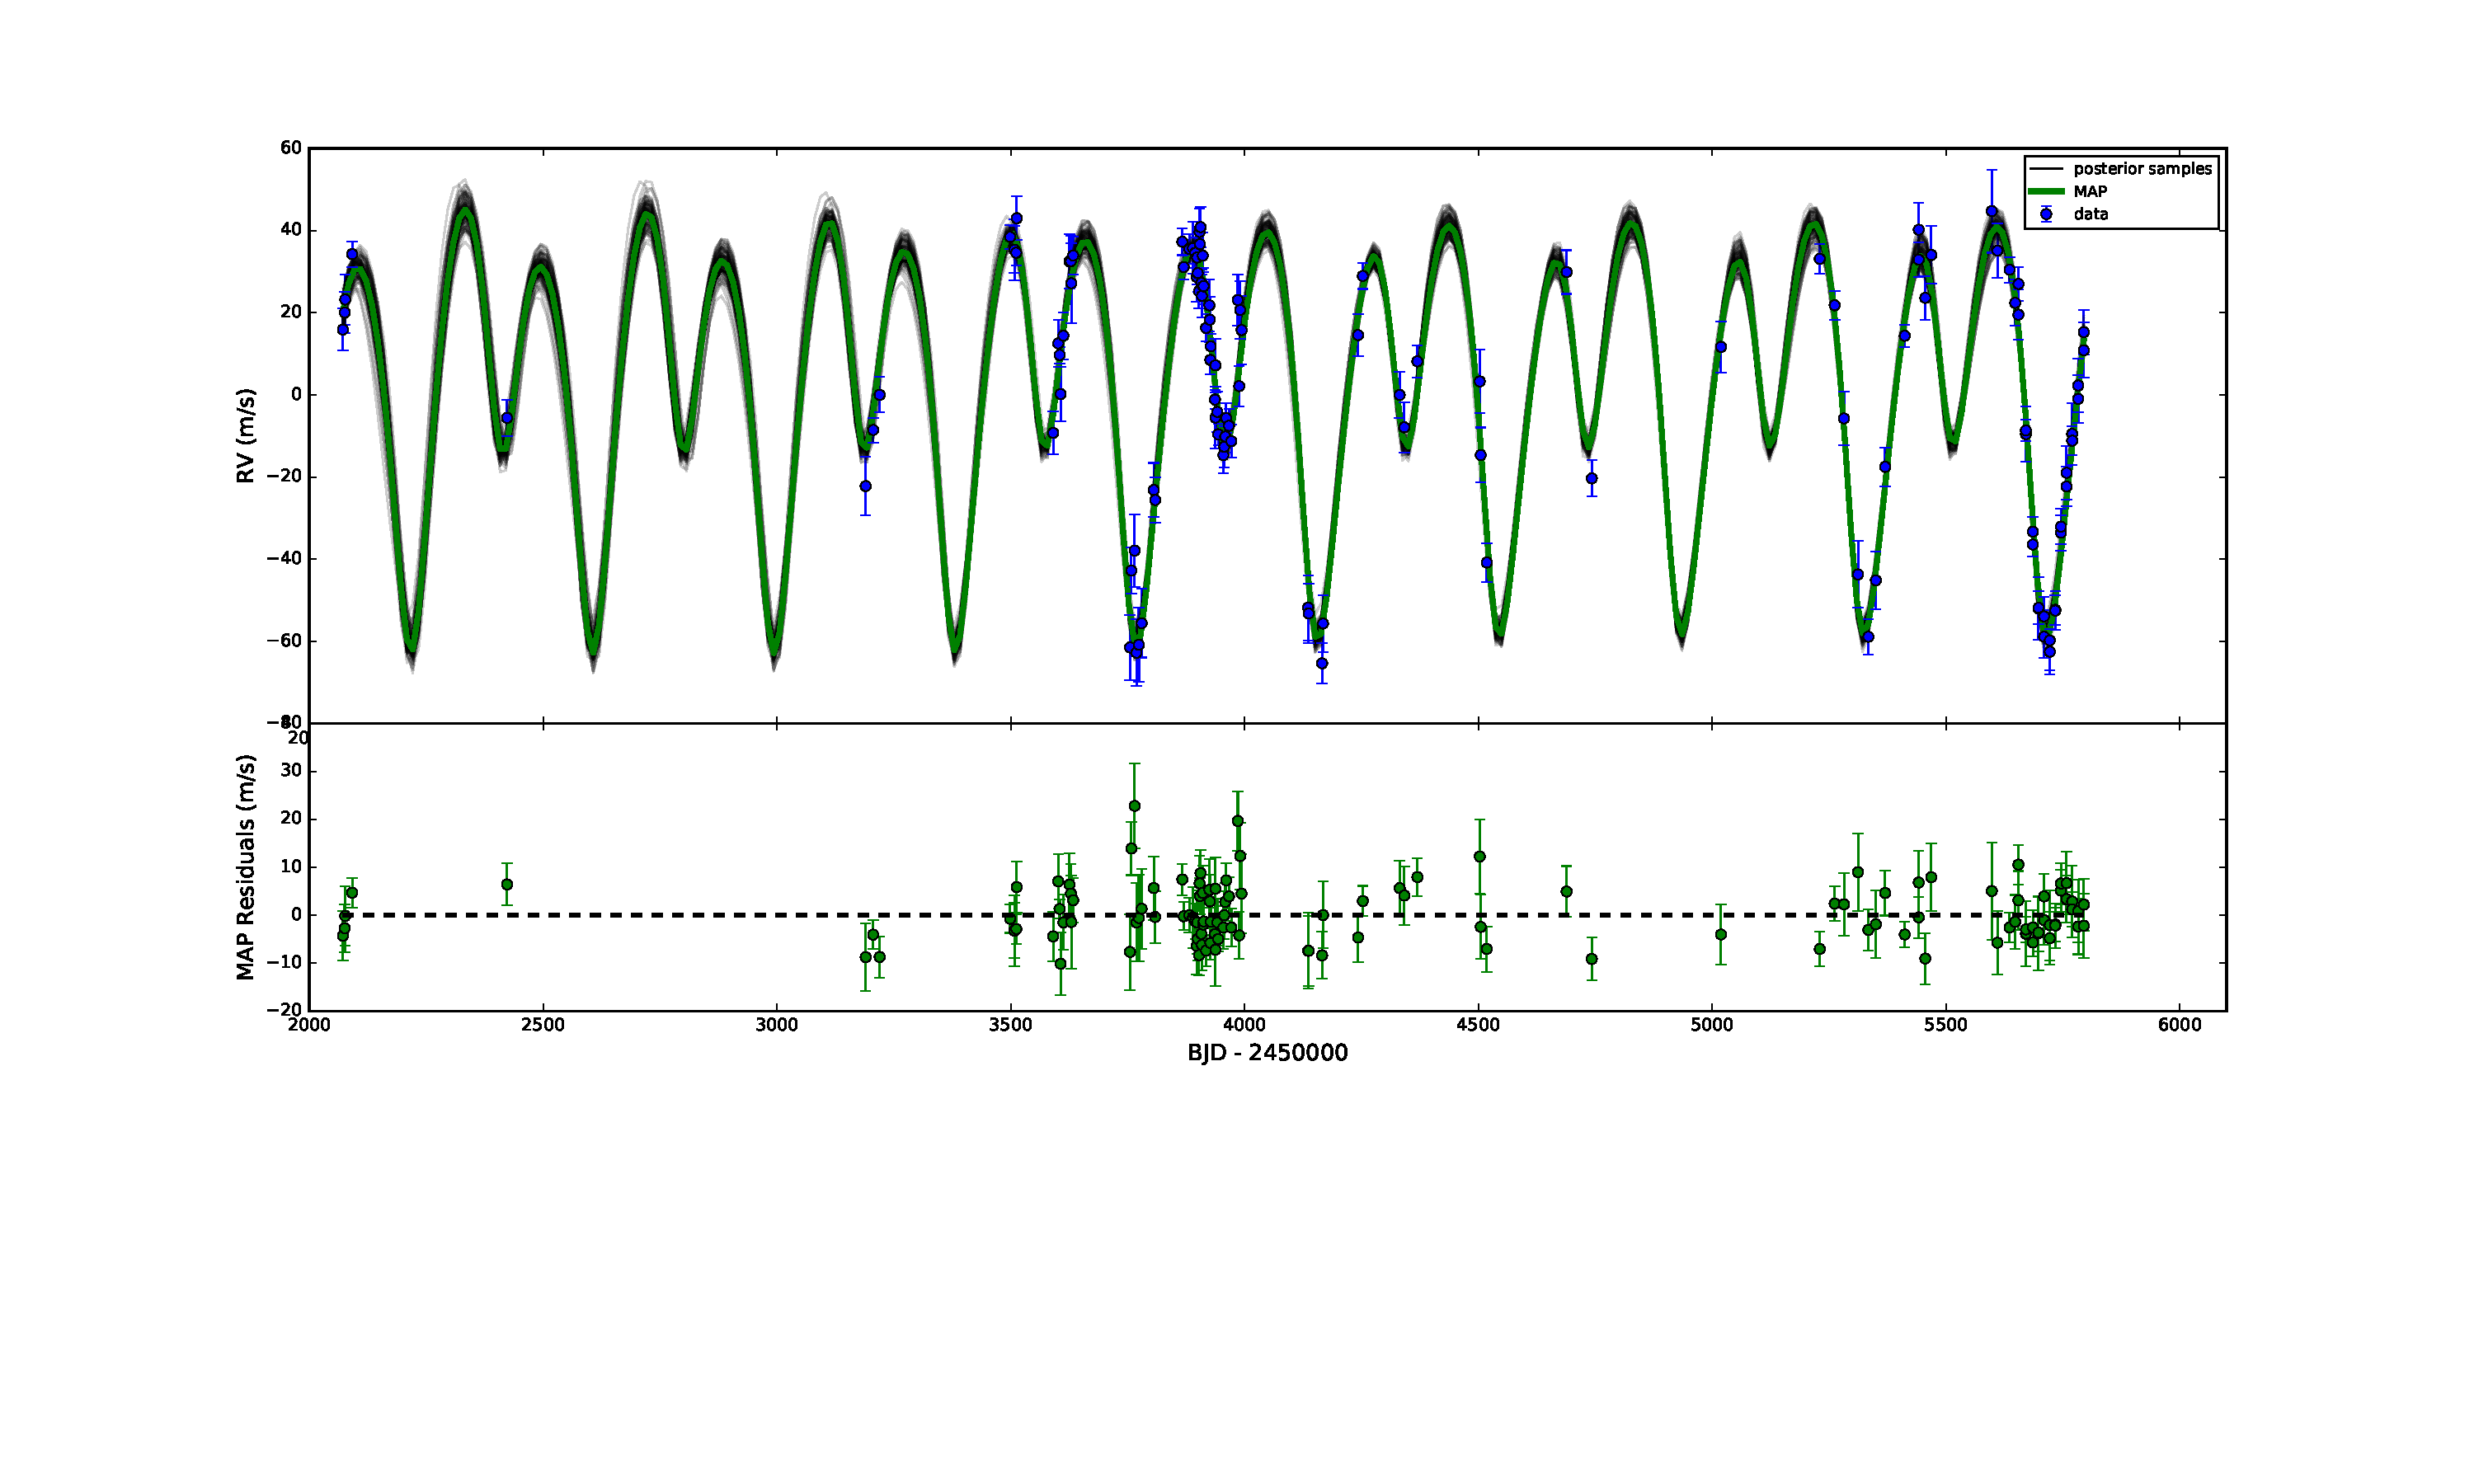
\includegraphics[trim=4.4cm 8cm 4.5cm 0cm, width=\textwidth]{chap6/images/hk_400walk_5000it_chkpt1_MAP_RV.pdf}
\caption{RV data and PPI model fit. 
Top panel shows the RV data points, MCMC MAP value (green), and 80 randomly plotted samples from the posterior (black). 
Bottom panel shows the residuals for the MAP fit to the RV data. 
 }
\label{fig:MCMC}
\end{figure*}

Our maximum a-posteriori (MAP) values for each parameter are displayed in Table~\ref{tab:MCMC}. 
For ease of comparison between our results and \R, we convert back into $e$ and $\omega$ variables from $h$ and $k$ variables.
Since we find $\sin(i)$ unconstrained in our MCMC analysis (see Figure~\ref{fig:stability}) it is not listed in Table~\ref{tab:MCMC}.
Parameters with subscript $1$ relate to the inner planet, while parameters with subscript $2$ relate to the outer planet. 
A random sample of 2000 draws from our PPI model's posterior distribution is shown in Figure~\ref{fig:stability}.

From Table~\ref{tab:MCMC} there are a few statistically significant differences between our PPI and noPPI models. 
In particular, $e_2$ is inconsistent at the $1$-$\sigma$ level, while $m_1\sin(i)$, $\omega_1$ and $M_1$ are inconsistent at the $2$-$\sigma$ level.
Furthermore, every parameter in our noPPI model is statistically consistent with \R.

\begin{table}
\begin{tabular}{llll}
\hline \hline
Parameter & PPI model & noPPI model & R2012\\ 
 \hline \hline
 $m_1\sin(i)$ ($M_J$) & $0.92 \pm 0.04$ & $0.82 \pm 0.04$ & $0.85 \pm 0.05$ \\ 
 $m_2\sin(i)$ ($M_J$) & $0.85 \pm 0.03$ & $0.87 \pm 0.03$ & $0.82 \pm 0.07$ \\ 
 $a_1$ (AU) & $0.641 \pm 0.002$ & $0.643 \pm 0.004$ & $0.64 \pm 0.01$ \\
 $a_2$ (AU) & $1.017 \pm 0.005$ & $1.015 \pm 0.007$ & $1.02 \pm 0.02$\\
 $e_1$ & $0.17 \pm 0.03$ & $0.18 \pm 0.03$ & $0.17 \pm 0.03$\\
 $e_2$ & $0.10 \pm 0.04$ & $0.20 \pm 0.05$ & $0.16 \pm 0.1$\\
 $\omega_1$ & $178^{\circ +14^{\circ}}_{\ \ -17^{\circ}}$ & $142^{\circ} \pm 13^{\circ}$ & $143^{\circ} \pm 11^{\circ}$\\
 $\omega_2$ & $241^{\circ +72^{\circ}}_{\ \ -65^{\circ}}$ & $189^{\circ +10^{\circ}}_{\ \ -16^{\circ}}$ & $180^{\circ} \pm 26^{\circ}$\\
 $M_1$ & $91^{\circ +15^{\circ}}_{\ \ -18^{\circ}}$ & $124^{\circ} \pm 15^{\circ}$ & $129^{\circ} \pm 0.7^{\circ}$\\
 $M_2$ & $178^{\circ +73^{\circ}}_{\ \ -66^{\circ}}$ & $244^{\circ +12^{\circ}}_{\ \ -17^{\circ}}$ & $233^{\circ} \pm 0.9^{\circ}$\\
 $\gamma$ (m/s) & $3.76 \pm 0.71$ & $3.70 \pm 0.70$ & --- \\
 $J$ (m/s) & $2.90^{+0.78}_{-0.64}$ & $2.92^{+0.78}_{-0.62}$ & $2.49$\\
 \hline
\end{tabular}
\caption{Best-fit model parameters from our MCMC samples. Our PPI model includes planet-planet interactions, while our noPPI model excludes planet-planet interactions. The derived parameters from \R are also listed for ease of comparison.}
\label{tab:MCMC}
\end{table}

In the top panel of Figure~\ref{fig:MCMC} we plot the MAP estimate for our PPI model, along with 100 randomly drawn samples from our posterior distribution.
In the lower panel the residuals between our MAP estimate and the RV data are shown. 
As can be seen, our PPI model represents a good fit to the data. 

We also try adding two additional parameters to our PPI model to account for mutual inclination between the planets.
For this inclination model we add $i_{x,2} = 2\textrm{sin}(i_2/2)\textrm{cos}(\Omega_2)$ and $i_{y,2} = 2\textrm{sin}(i_2/2)\textrm{sin}(\Omega_2)$, where $i_2$ is the inclination of the outer planet (with respect to the inner planet and star) and $\Omega_2$ is the longitude of ascending node of the outer planet \citep{Pal2009}. 
The mutual inclination returned by this model is $i_2 = 30^{\circ +22^{\circ}}_{\ \ -37^{\circ}}$, being consistent with 0 and ruling out large mutual inclinations. 
Comparing this inclination model to our original PPI model using a posterior odds ratio (see Section~\ref{sec:MC}) yields a value of 0.4, indicating a slight preference over the inclination model.
Since our original PPI model is simpler and the model parameters between models are similar, we choose to stick with our PPI model for the remainder of our analysis. 

%%%%%%%%%%%%%%%%%%%%%%%%%%%%%%%%%%%%%%%%%%%%%%%%%%%

\subsection{Resonance Analysis}
Using our posterior samples found in Section~\ref{sec:Results}, we can assess the likelihood that the planets orbiting HD155358 are in 2:1 MMR. 
More specifically, we can draw samples from the posterior distribution and calculate what fraction of these systems have librating resonant angles. 
The resonant angles are calculated according to:
\begin{align*}
\begin{split}
\phi_1 &= (j - 1)\lambda_1 - j\lambda_2 + \omega_1 \\
\phi_2 &= (j - 1)\lambda_1 - j\lambda_2 + \omega_2 
\end{split}
\end{align*}
where $\lambda$ is the mean longitude, $\omega$ is the argument of periapsis, and $j$ is the order of the resonance ($j=2$ for this work).
Our aim is to use the fraction of systems with librating resonant angles as a measure of how likely the system is to be in MMR. 
% We acknowledge that librating resonant angles do not guarantee that a system is in MMR \citep[e.g.][]{Delisle2012}, however, as a first order approximation this criteria is sufficient.

For each set of parameters drawn from our posterior we simulate the corresponding system for 4000 years with a timestep equal to $P_1/50$. 
Over the course of a given simulation we generate 1000 equally spaced outputs for each resonant angle, and classify a resonant angle to be librating if the difference between the maximum and minimum is less than a threshold value $\kappa$. 
We set $\kappa = 7\pi/4$ since this allows for large resonant libration amplitudes while also ensuring that misclassification of librating/non-librating systems is low. 
Our results are insensitive to nearby values of $\kappa$ (e.g. $5\pi/3$, $9\pi/5$, etc.).
We check for librations around both 0 and $\pi$.

\begin{table}
\begin{tabular}{p{2cm}p{1.8cm}p{1.8cm}}
\hline \hline
 & PPI model & noPPI model \\\hline
$\phi_1$ librating & $98\% \pm 6\%$ & $1\% \pm 6\%$ \\
$\phi_2$ librating & $5\% \pm 6\%$ & $1\% \pm 6\%$ \\
%Unstable & $0\% \pm 6\%$ & $40\% \pm 6\%$ \\
 \hline \hline
\end{tabular}
\caption{
The percent of randomly drawn samples with $\phi_1$ and $\phi_2$ librating, for our PPI and noPPI models. 
Error bars calculated from simple Poisson statistics. 
}
\label{tab:res}
\end{table}

Our results are presented in Table~\ref{tab:res} for our PPI and noPPI models, for 300 samples randomly drawn from each posterior distribution. 
The error bars are calculated from simple poisson statistics.
For our PPI model, almost every drawn sample has $\phi_1$ librating, strongly suggesting that the system is in MMR. 
In contrast, our noPPI model shows no evidence of librating resonant angles.

Given our analysis, there is a high likelihood that the HD155358 system is in MMR, and is therefore likely to have formed via planet migration, as we show in the next section.

%%%%%%%%%%%%%%%%%%%%%%%%%%%%%%%%%%%%%%%%%%%%%%%%%%%
%%%%%%%%%%%%%%%%%%%%%%%%%%%%%%%%%%%%%%%%%%%%%%%%%%%
\section{Formation via Migration}
\label{sec:form}
\subsection{Methods}
We now use the results found in the previous section to explore the formation of HD155358 via migration.
We use a simple model by which the outer planet is migrated into 2:1 MMR using a parametric model, mimicking the presence of a protoplanetary disk.
Specifically, we introduce semi-major axis and eccentricity damping timescales, $\tau_a = a/\dot{a}$ and $\tau_e = e/\dot{e}$, respectively, where the two are related by a constant $K = \tau_a / \tau_e$. 
We refer to this class of convergent-migration models as ``CM models". 

We follow the implementation by \cite{Papa2000} and add an additional acceleration on each planet according to:
\begin{align*}
\begin{split}
\textbf{a}_{\rm mig} &=  -\frac{\textbf{v}}{\tau_a} \\
\textbf{a}_{\rm damp} &= -2\frac{(\textbf{v}\cdot\textbf{r})\textbf{r}}{r^2\tau_e},
\end{split}
\end{align*}
where $\textbf{v}$ is the velocity and $\textbf{r}$ is the position of the planet relative to the star. 
The migration prescriptions of \citet{Papa2000} were designed with Type-I migration in mind, yet our planets likely lie in the Type-II migration regime.
However, since we are interested primarily in seeing whether a simple migration model can reproduce the data, this model choice will suffice. 
More accurate, 3-D hydrodynamical simulations of Type-II planetary migration are significantly more complex and beyond the scope of this chapter. 

For each simulation three parameters are independently varied -- the eccentricity damping timescale of the inner planet $\tau_{e_1}$, the eccentricity damping timescale of the outer planet, $\tau_{e_2}$, and the migration timescale of the outer planet, $\tau_{a_2}$.
The inner planet does not undergo migration by itself, i.e. $\tau_{a_1} = \infty$.
Initial values for $\tau_{a_2}$ are drawn from a uniform distribution in log-space between $10^{2.5}$ and $10^7$ years, while initial values for $K_1$ and $K_2$ are drawn between $10^{-1}$ and $10^3$.
Planet masses are drawn from our posterior distribution (Section~\ref{sec:Results}), all eccentricity and inclination values are initialized to zero, and the remaining orbital parameters are randomly drawn from uniform distributions. 

When planets migrate into MMR in the presence of a protoplanetary disk an equilibrium eccentricity $e_{eq}$ is reached, representing a stable balance between migration excitation and protoplanetary disk damping \citep[e.g.][]{Goldreich2014}. 
For each simulation we migrate the outer planet inwards for a time of $T_{\rm mig} = 5\tau_a$ years, after which $e_{eq}$ has reached a stable value. 
In cases where $T_{\rm mig} < 5000$ years we extend the simulation time to $T_{\rm mig} = 5000$ to ensure a stable solution. 
The migration parameters $\tau_{a_1}$, $\tau_{e_1}$ and $\tau_{e_2}$ are then logarithmically increased to $10^7$ years over the same amount of time ($T_{\rm mig}$), mimicking the dispersal of the protoplanetary disk. 
Simulations are independently checked to ensure that a) an equilibrium eccentricity is reached over $T_{\rm mig}$, and b) the disk dispersal is done adiabatically, ensuring that the resonance is not abruptly changed during the increase of $\tau_{a_1}$, $\tau_{e_1}$ and $\tau_{e_2}$.
Simulations that do not fulfill this criteria are discarded.

Once migration is turned off, a RV curve is generated from the simulation and fit to the original RV data using \emcee as before, but now with only five free parameters: 
$t_s$, a parameter allowing the rescaling of the orbital periods, 
$t_t$, a parameter accounting for an offset in time, 
$y_s$, a RV-stretch parameter to account for amplitude offsets (effectively rescaling the masses of both the planets and the star, while keeping the mass ratios and periods constant).
As in the original analysis, we also include  
$\gamma$, an offset parameter to account for any stellar drift along the line of sight, and 
$J$, a jitter parameter to account for underestimated measurement noise and intrinsic stellar noise in the RV data.
Each \emcee fit is run for an initial burnin phase of 200 steps with 100 walkers, after which the walkers are resampled near the best solution and run for 2000 steps. 

%%%%%%%%%%%%%%%%%%%%%%%%%%%%%%%%%%%%%%%%%%%%%%%%%%%

\subsection{Model Comparison}
\label{sec:MC}
In a Bayesian sense, each simulation represents a different model $M$ characterized by $\theta_{\rm model}$ = \{$\tau_{a_1}$, $K_1$, $K_2$\}, with each model having a unique MAP estimate for its parameters $\theta_{fit}$ = \{$t_s$, $t_t$, $y_s$, $\gamma$, $J$\}.
Note that our analysis thus incorporates the fact that many different models might explain the data equally well. 
A single model with parameters $\theta$ = $\{\tau_{a_1}$, $K_1$, $K_2$, $t_s$, $t_t$, $y_s$, $\gamma$, $J$\} on the other hand would make MCMC convergence more difficult. 

When multiple models can explain the data, the posterior odds ratio can be used to determine if there is any preference for one model over another. 
The posterior odds ratio, $P_{ij}$, is calculated according to \citep{Gregory2005}:
\begin{equation}
P_{ij} = \frac{p(M_i)}{p(M_j)} \frac{p(D|M_i)}{p(D|M_j)}, 
\label{eq:PO}
\end{equation}
where $p(M)$ is the prior odds for model $M$, and $p(D|M)$ is the marginal (or global) likelihood for model $M$.
The ratio of marginal likelihoods for two competing models is also known as Bayes' factor. 
In our case, the ratio of prior odds is unity since we have no prior model preference. 
Thus, the posterior odds ratio is equivalent to calculating Bayes' factor.

Formally, the marginal likelihood is calculated by marginalizing over the parameters $\theta$ of a model according to \citep{Gregory2005}:
\begin{equation}
p(D|M) = \int p(\theta|M)p(D|\theta,M)d\theta = \Lagr(M)
\label{eq:GL}
\end{equation}
where $p(D|\theta, M)$ is the likelihood and $p(\theta|M)$ is the prior. 
The marginal likelihood represents the probability of the data given the model. 

\begin{figure*}
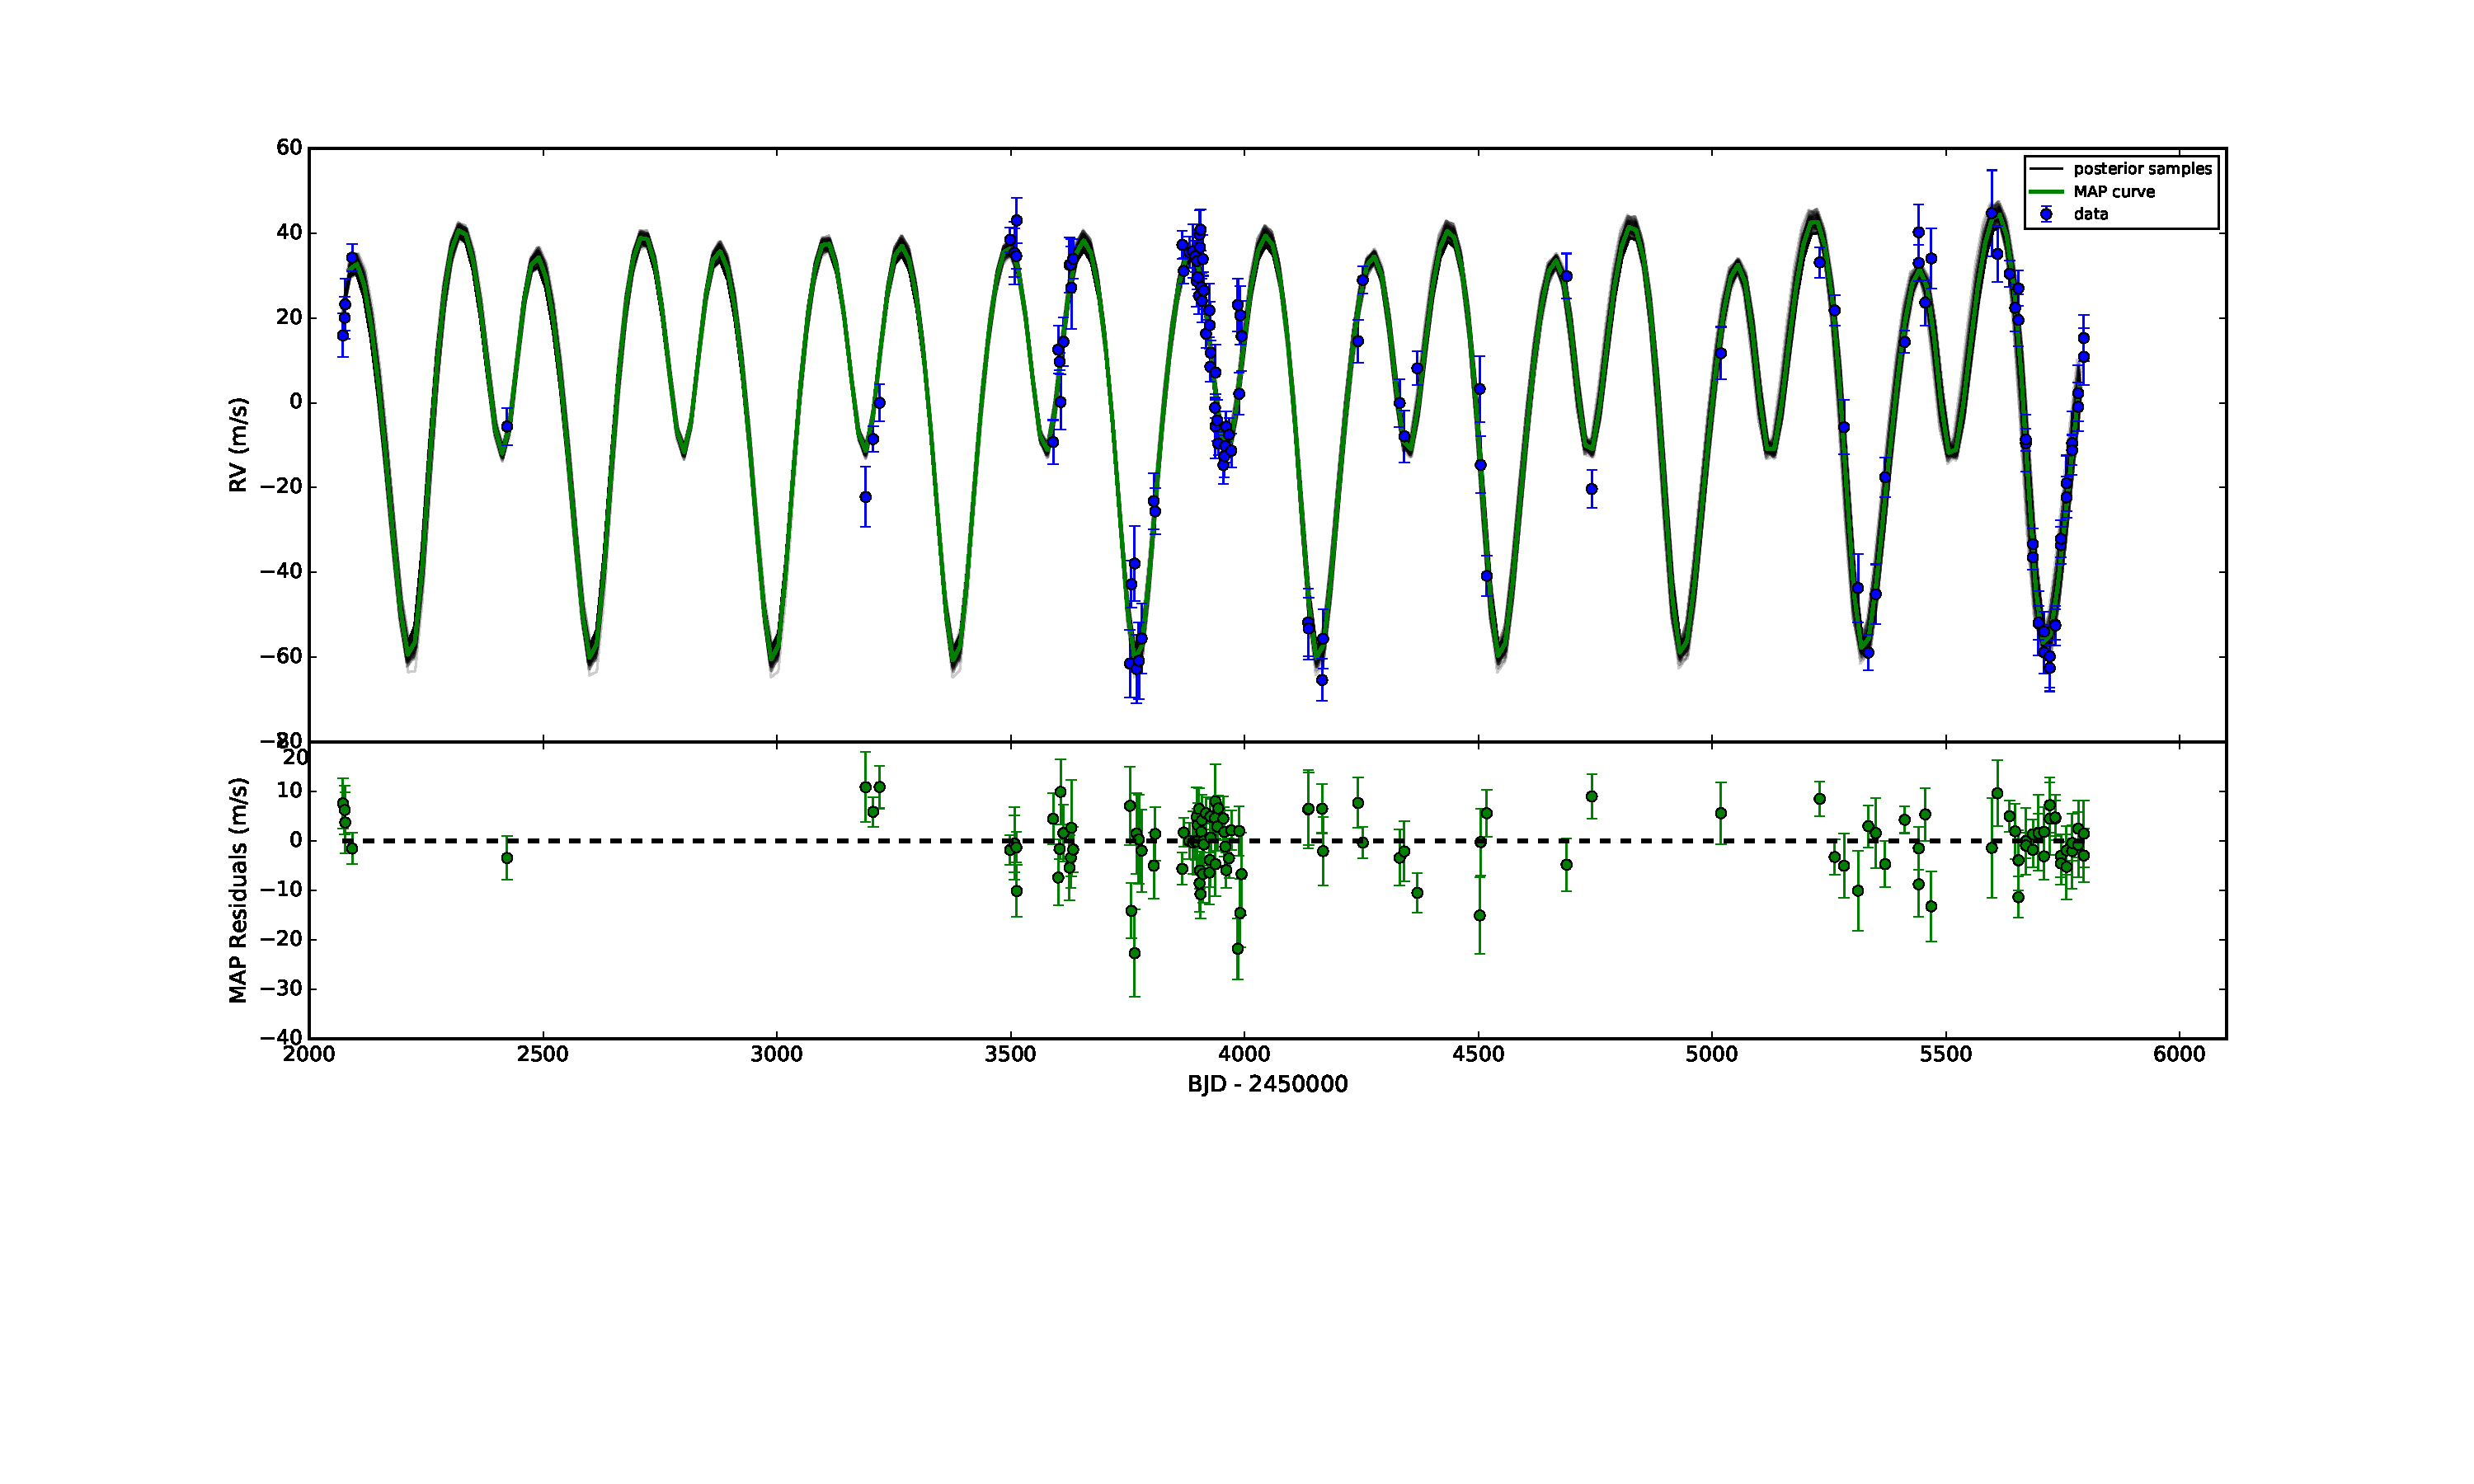
\includegraphics[trim=4.4cm 7cm 4.5cm 0cm, width=\textwidth]{chap6/images/taueinner_migrate3e+03_Kin7e+00_Kout3e+02_sd931.pdf}
\caption{RV data and $\theta_{\rm mig,best}$ fit.
Top panel shows the RV data points, MCMC MAP value (green), and 80 randomly plotted samples from the posterior (black). 
Bottom panel shows the residuals for the MAP fit to the RV data. 
 }
\label{fig:bestform}
\end{figure*}

\begin{figure}
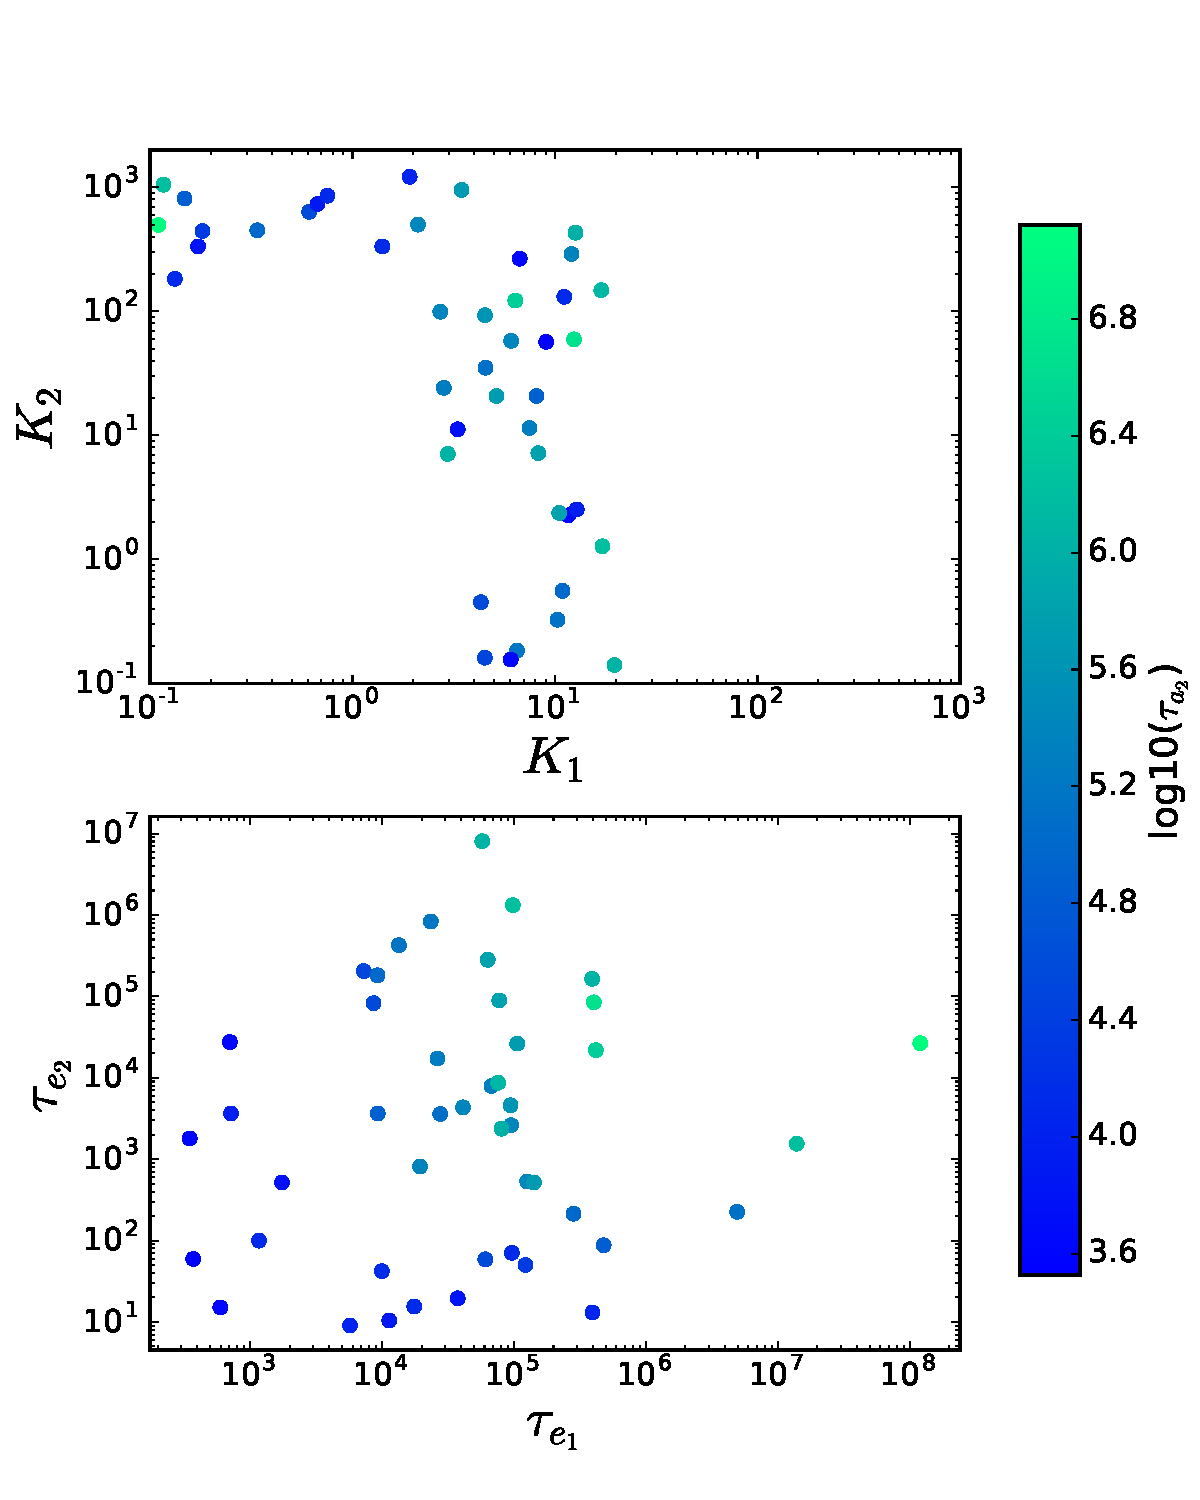
\includegraphics[width=\columnwidth]{chap6/images/plot_good_ones.pdf}
\caption{The best 45 models $\theta_{\rm model}$ = \{$\tau_{a_1}$, $K_1$, $K_2$\} with Bayes' factors less than 100 when compared against the best model in our sample of 3000 simulations. 
Top panel presents the data in ($K_1$, $K_2$) space, and the parameters from our 3000 simulations were uniformly sampled from the region displayed. 
Bottom panel displays the same data in ($\tau_{e_2}$, $\tau_{e_2}$) space. 
Colour indicates the log value of $\tau_{a_1}$.
 }
\label{fig:goodones}
\end{figure}

When the marginal likelihood is normally distributed with flat priors, Eq.~\ref{eq:GL} can be approximated as \citep{Kass1995, Gregory2005}:
\begin{equation}
\Lagr(M) \approx \Lagr(\hat{\theta}) (2\pi)^{d/2} |\Sigma|^{1/2} \Delta \theta
\label{eq:Lapprox}
\end{equation}
where $\Lagr(\hat{\theta})$ is the the maximum likelihood, $d$ is the number of parameters in model $M$, $\Sigma$ is the covariance matrix of the posterior distribution, and $\Delta \theta = \prod_i^d 1/\delta \theta_i$ is the product of prior probabilities normalized by their lengths $\delta \theta$.
Since all models have the same flat priors for each parameter, Eq.~\ref{eq:PO} becomes:
\begin{equation}
P_{ij} = \frac{\Lagr_i(\hat{\theta}) |\Sigma_i|^{1/2}}{\Lagr_j(\hat{\theta}) |\Sigma_j|^{1/2}}
\label{eq:POapprox}
\end{equation}

Since \emcee returns both the samples and log-likelihoods at each step in the MCMC chain, it is straightforward to calculate the posterior odds ratio using Eq.~\ref{eq:POapprox}. 

%%%%%%%%%%%%%%%%%%%%%%%%%%%%%%%%%%%%%%%%%%%%%%%%%%%

\subsection{Results}
\label{sec:formresults}

Our best model from a sample of 3000 simulations is plotted in Figure~\ref{fig:bestform}, corresponding to $\theta_{\rm model, best}$ = ($\tau_{a_2}$, $K_1$, $K_2$) = (4000 years, 7, 265).
In the top panel we plot the MAP estimate along with 100 randomly drawn samples from our posterior distribution.
In the lower panel the residuals between our MAP estimate and the RV data are shown. 
As can be seen, our model represents a good fit to the data. 

Following \citet{Kass1995}, a posterior odds ratio lower than 100 indicates no decisive preference for one model over another, and in Figure~\ref{fig:goodones} we plot competing models which, when compared to $\theta_{model,best}$, yield a posterior odds ratio of less than 100. 
The top panel in Figure~\ref{fig:goodones} presents the valid models in ($K_1$, $K_2$, $\tau_{a_2}$) space, while the bottom panel presents them in ($\tau_{e_1}$, $\tau_{e_2}$, $\tau_{a_2}$) space. 
Although many different migration models are able to explain the data, regions of parameter space appear to be ruled out.
In the top panel of Figure~\ref{fig:goodones}, ($K_1 < 3$, $K_2 < 100$) and $K_1 > 20$ are two regions that appear to be ruled out by the data. 
In the bottom panel, positive correlation can be seen between $\tau_{a_2}$ and $\tau_{e_1} + \tau_{e_2}$.

%%%%%%%%%%%%%%%%%%%%%%%%%%%%%%%%%%%%%%%%%%%%%%%%%%%
%%%%%%%%%%%%%%%%%%%%%%%%%%%%%%%%%%%%%%%%%%%%%%%%%%%
\section{Stability}
\label{sec:stability}
\begin{figure*}
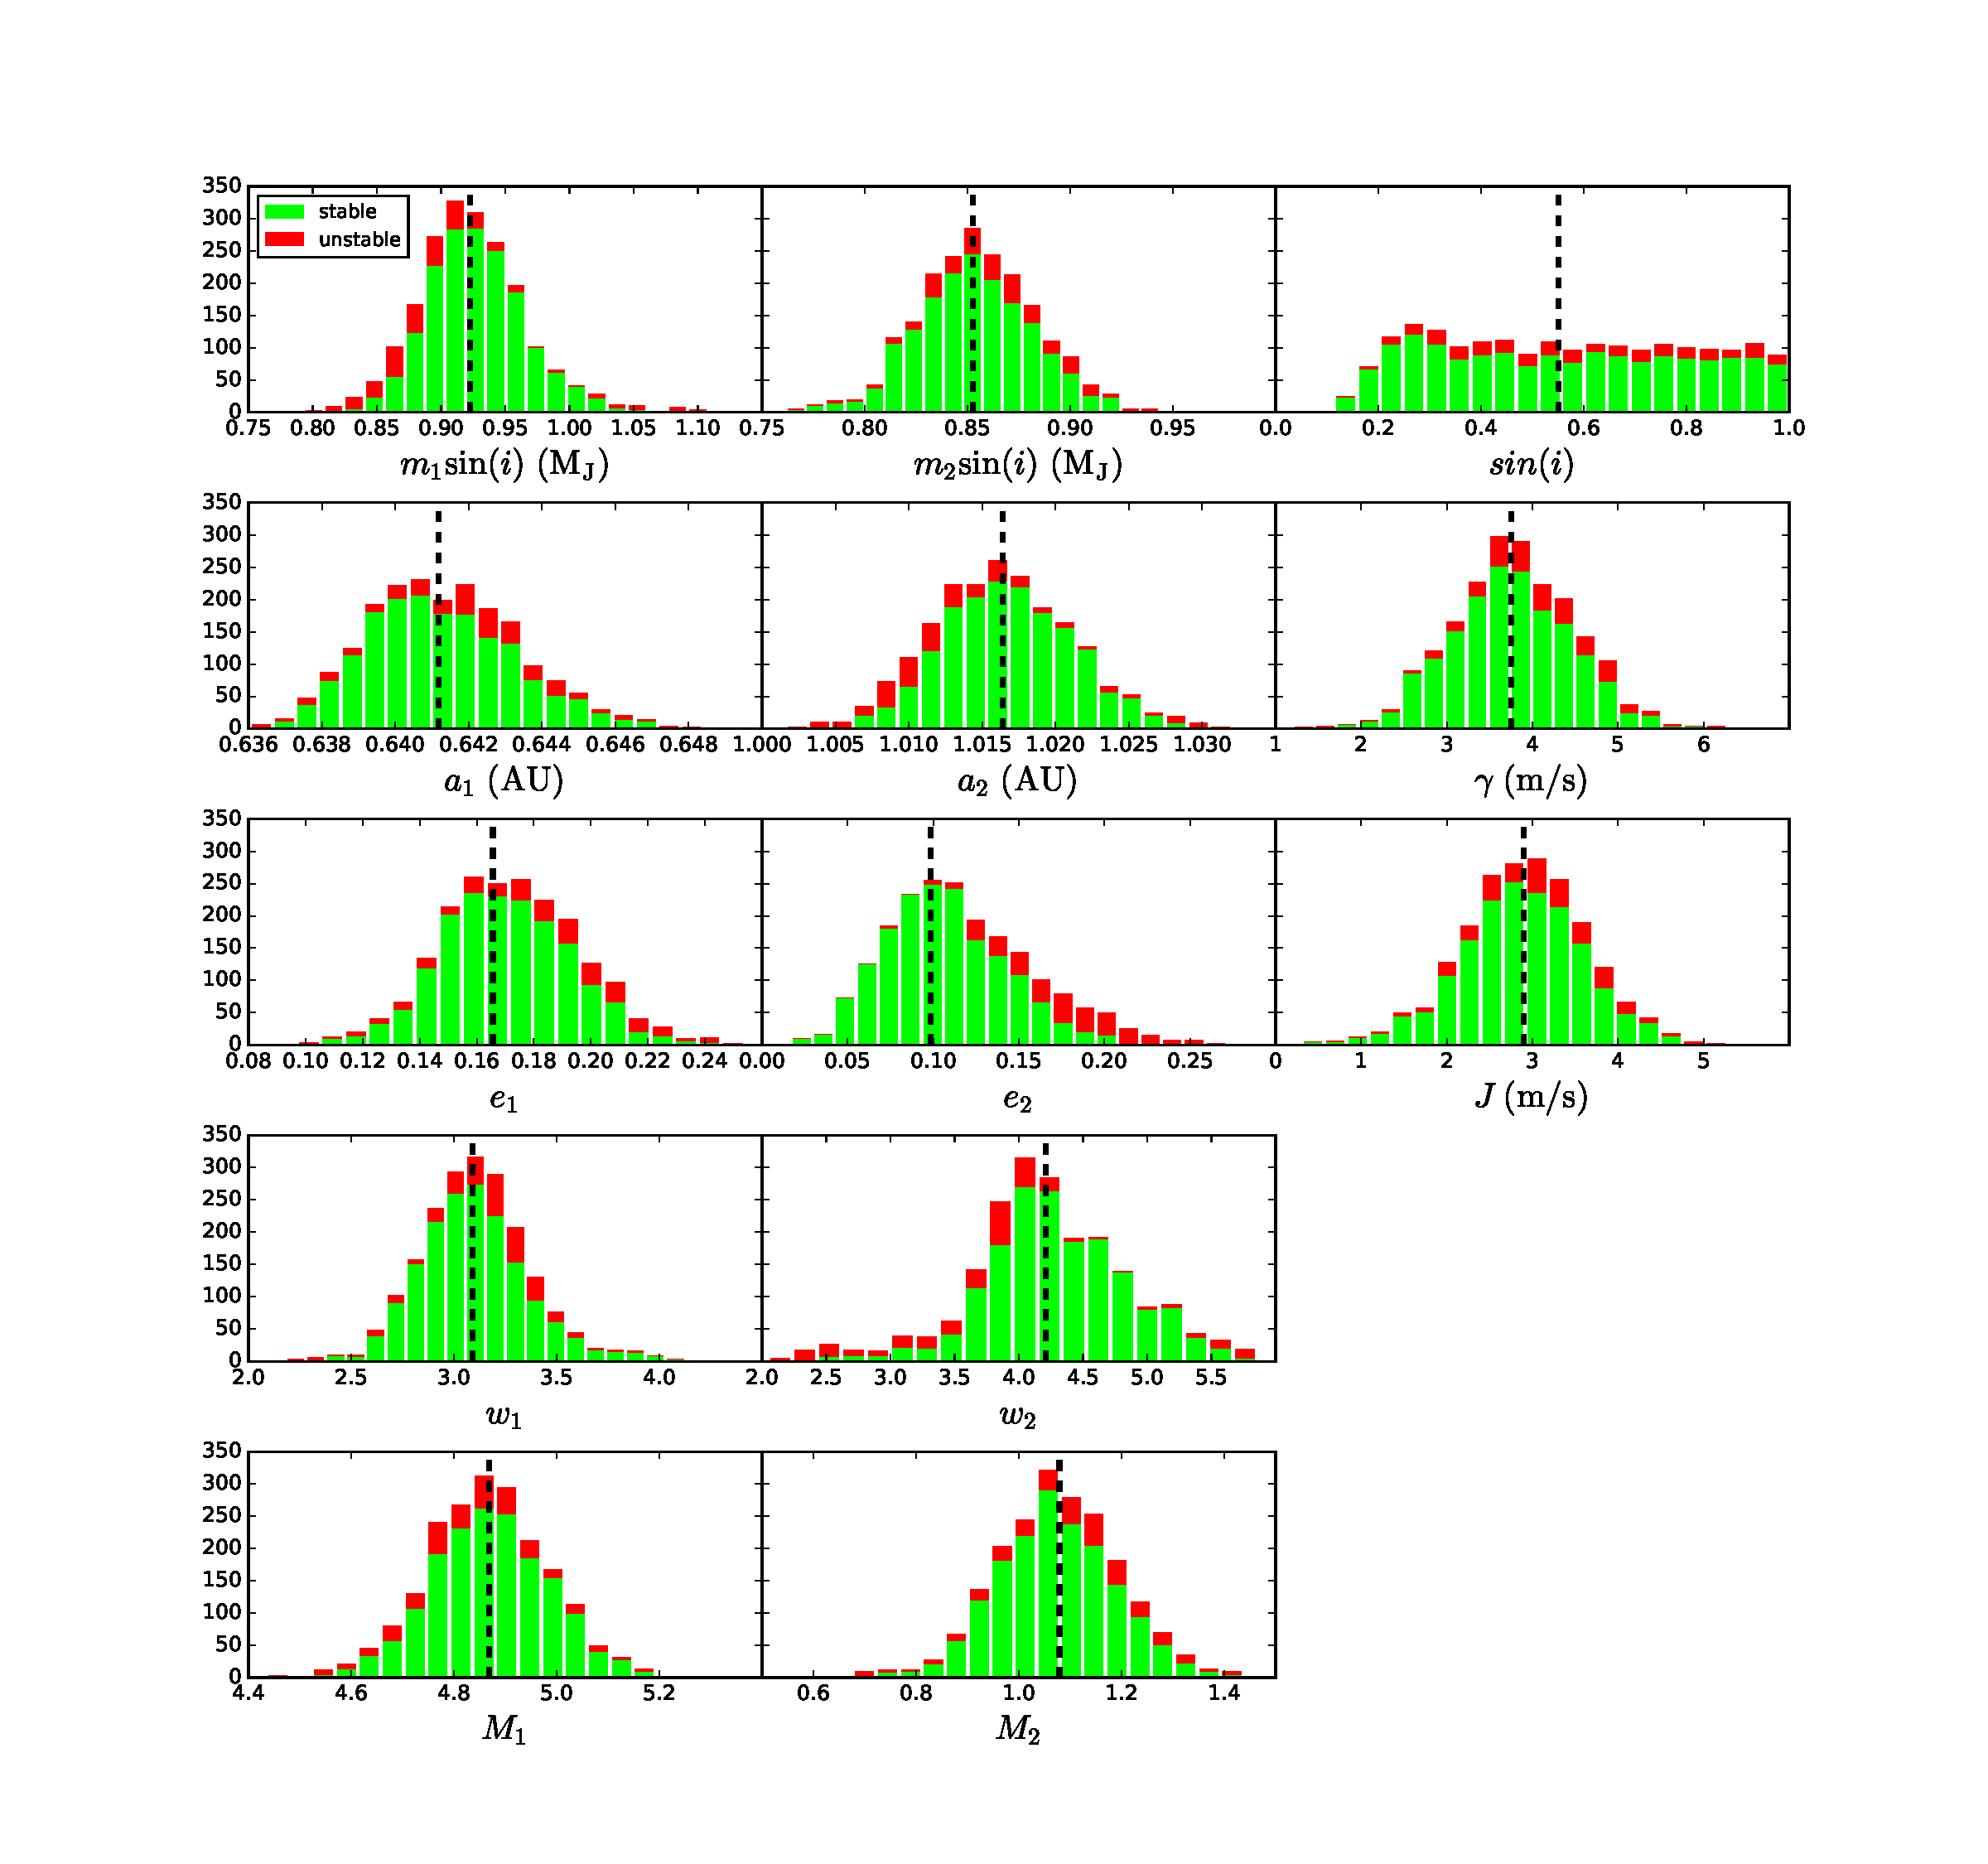
\includegraphics[trim=4.4cm 2cm 4.5cm 0cm, width=\textwidth]{chap6/images/stability_plot_histogram}
\caption{
    Histograms of each parameter showing the distribution of 2000 stable (green) and unstable (red) systems drawn from our PPI model's posterior distribution and simulated for $10^9$ years.
The black vertical dashed line in each histogram represents our MAP estimate for that parameter. 
 }
\label{fig:stability}
\end{figure*}
Following \citet{Marshall2010} and \cite{Horner2011}, \R conducted a stability analysis by holding the inner planet constant at the best-fit values and varying the outer planet's orbital parameters randomly over a 3$\sigma$ range in $a$, $e$, $\omega$ and $M$. 
However, drawing parameters in this manner does not preserve their correlations, and it is possible to draw parameter combinations that are inconsistent with the RV data. 
\R also kept the planet masses fixed at their minimum $m\sin(i)$ values, precluding the possibility of further constraining the masses from the stability analysis. 

In a Bayesian framework, we can simply draw parameters from the posterior distribution and simulate them for a desired length of time. 
Parameter correlations are naturally preserved in the posterior distribution, and a probability of longterm stability can be easily found. 

In this study we draw 2000 random samples from our PPI model's posterior distribution and simulate the subsequent evolution for $10^9$ years using \whfast with a timestep of $P_1$/200. 
We also make use of the {\tt Simulation Archive} \citep{Rein2017} for stopping, restarting and analyzing simulations. 
The relative energy error for all stable simulations remains bounded at $< 10^{-7}$.

The results are presented in Figure~\ref{fig:stability} as a histogram for each parameter.
Stable and unstable systems over $10^9$ years are marked in green and red, respectively, while our MAP values from our PPI model is shown as vertical, black, dashed lines. 
$83\% \pm 2\%$ of our samples are stable over $10^9$ years and our MAP values land in highly stable regions, indicating that our PPI model is longterm stable. 

Unstable systems appear to be clustered in certain regions of parameter space.
As can be seen in Figure~\ref{fig:stability}, $m_1\textrm{sin}(i)<0.87$, $e_2>0.15$, $a_2<1.01$ AU and $\omega_2<4$ are regions where there are a significant fraction of unstable systems.
It is therefore unlikely that the true planet parameters lie in these regions. 

These unstable regions are consistent with the results found in \R, however, unlike \R our best-fit values are centred in highly stable regions (see Figures 9 and 10 in \R for a comparison). 
Although not shown, we find no clustering of unstable systems in ($m_1$, $m_2$) space, and thus the planet masses cannot be further constrained via stability analysis.  

%%%%%%%%%%%%%%%%%%%%%%%%%%%%%%%%%%%%%%%%%%%%%%%%%%%
%%%%%%%%%%%%%%%%%%%%%%%%%%%%%%%%%%%%%%%%%%%%%%%%%%%
\section{Discussion and Conclusion}
\label{sec:conc}
In this work we used three different model types to analyze the RV curve of HD155358 -- the PPI, noPPI and CM models. 
Our PPI (planet-planet interactions) and noPPI (no planet-planet interactions) models fit the RV curve to a model parameterized by the orbital elements of each planet (Section~\ref{sec:orb}), while our CM model was parameterized by migration parameters and fit this result to the RV curve (Section~\ref{sec:form}).
The best-fit parameters from our PPI and noPPI models are shown in Table~\ref{tab:MCMC}, while Table~\ref{tab:res} shows that there is a high likelihood that the planets of HD155358 are in MMR. 

The noPPI model is an approximation to the PPI model, and we have shown in Section~\ref{sec:Results} that planet-planet interactions are strong enough in the HD155358 system to yield differing conclusions about the resonant structure. 
More specifically, our PPI model predicts a high likelihood that the planets are in MMR, while our noPPI model predicts a low likelihood that the planets are in MMR. 
Since planets in MMR are highly likely to have formed via migration, by extension the PPI and noPPI models have different formation implications. 
Quantitatively, the orbital parameters returned by our PPI and noPPI models differ by up to $2\sigma$.

Our CM model has demonstrated that formation models of this style can be used to fit RV curves and constrain the initial conditions of a given system. 
One possibility for future work is to make the CM model more sophisticated, for example by modelling the planet-disk interactions in more realistic hydrodynamic simulations \citep{Rein2010}. 
With such a model, one could place further constraints on the formation of HD155358.

From a frequentist's point of view, the reduced $\chi^2$ values for our PPI, noPPI and best CM model are 1.4, 1.6 and 0.7 respectively, indicating that all three models are capable of fitting the data well.
However, our PPI model should be considered the only valid model when it comes to determining the true values of the observed system.
We also performed a stability analysis on our PPI model, finding that $83\% \pm 2\%$ of samples drawn from our posterior are stable over $10^9$ years.
We find regions of stable and unstable parameter space similar to \R, however unlike \R our best-fit model solution is centred in a stable region. 

\chapter{Conclusions \& Future Work}
\section{Summary}
This thesis dealt with the statistics, formation and stability of exoplanetary system. 

In Chapter~\ref{chap:Stats}, I performed a general analysis of the \kep catalog using the \citet{Ramirez2014} data to calculate the occurrence rate of small planets, accounting for detection biases and radius errors. 
Here I found that Kepler planets are preferentially peaked at $2-2.8R_\oplus$, with their numbers decreasing gradually toward smaller sizes, with a roughly log-uniform period distribution.
The average number of planets per star with periods between $20$ and $200$ days and radii between $1$ and $4R_\oplus$ is $0.46 \pm 0.03$. 
Such planets have likely experienced little photoevaporation, and may reflect the "primordial" planet population. 
Upon extrapolation I obtained an occurrence rate for Earth-like planets within the "habitable zone" (as calculated by 1-D climate models) of $6.4^{+3.4}_{-1.1}\%$. 

Through my analysis of the \kep catalog in Chapter~\ref{chap:Stats}, I became interested in the statistical excess of planets wide of MMR, motivating the work in Chapter~\ref{chap:Tides}.
Here I used optimistic theoretical estimates for the minimum initial eccentricity required to explain the offset of \kep planets from MMR due to tidal forces alone, complimenting these calculations with N-body simulations.
Analyzing 27 \kep systems having planets within $6\%$ of the 2:1 MMR, I found that the initial eccentricities required to explain the observed spacings due to tides alone are unreasonable from simple dynamical arguments.
Furthermore, our numerical simulations revealed "resonant tugging", an effect which conspires against the migration of resonant planets away from the 2:1 MMR, requiring even higher initial eccentricities in order to explain the current \kep distribution. 
In summary, I found that tides alone cannot explain planets close to 2:1 MMR, and additional mechanisms are required to explain these systems. 

After my work in Chapter~\ref{chap:Tides}, I sought other mechanisms capable of transporting planets from MMR. 
Planetesimals are a promising candidate for transporting planets from MMR, motivating my work in Chapter~\ref{chap:Hermes} where I presented \hermes, a new hybrid integration scheme for long-term simulations of planetary systems undergoing close encounters or planetesimal-driven migration. 
Distant particles are integrated using \whfast, while close particles are integrated with \ias.
In addition, I created an adaptive routine for optimizing the close encounter boundary to help maintain accuracy whilst close encounters are occurring.
Since \whfast is symplectic, \ias is accurate to machine precision and both of them are unbiased, the energy error grows sub-linearly with time under the assumption that either impact parameters are randomly distributed or close encounters are rare.
I found that \hermes provides a good balance between speed and accuracy, neither achieved by the individual symplectic or non-symplectic integrators alone.

In addition to my work analyzing \kep planets, I have also been taking part in machine learning workshops held frequently at the Centre for Planetary Science. 
From these workshops, a group of us became interested in applying machine learning to the problem of planetary stability. 
In Chapter~\ref{chap:Stability} we showed that characterizing the complicated and multi-dimensional stability boundary of tightly packed systems is amenable to machine learning methods. 
In particular, training a state-of-the-art machine learning algorithm on physically motivated features yields an accurate classifier of stability in packed systems. 
On the stability timescale I investigated ($10^7$ orbits), our trained machine was 3 orders of magnitude faster than direct N-body simulations. 
Optimized machine learning classifiers for dynamical stability may thus prove useful across the discipline, e.g., to characterize the exoplanet sample discovered by the upcoming Transiting Exoplanet Survey Satellite (TESS).

Finally, my previous research experience motivated me to work on the planetary system HD155358, since it drew on a number of familiar topics like MMR, formation and stability. 
In Chapter~\ref{chap:HD155358}, I analyzed the RV data for the star HD155358, which hosts two Jovian-sized planets near 2:1 MMR. 
Using a Bayesian model parameterized by the orbital elements of each planet, I showed that excluding planet-planet interactions can yield statistically different orbital solutions, leading to different implications for formation and stability. 
Using our updated orbital solution I calculated a high likelihood that the planets are in MMR. 
In addition, I conducted a stability analysis by drawing samples from our posterior distribution and simulating them for $10^9$ years, finding that our best-fit values land firmly in a stable region of parameter space.
I also explored a series of formation models that migrate the planets into MMR and generated synthetic RV curves to fit directly to the observed data. 
I found that a number of formation models fit the RV data surprisingly well, with some migration parameters being ruled out.

%%%%%%%%%%%%%%%%%%%%%%%%%%%%%%%%
\if{false}
\section{Summary of Results}
\subsection{Occurrence Rate of \kep Planets}
In Chapter~\ref{chap:Stats} we used the \citet{Ramirez2014} \kep catalog to calculate the occurrence rate of small planets, accounting for detection biases and radius errors. 
We found that Kepler planets are preferentially peaked at $2-2.8R_\oplus$, with their numbers decreasing gradually toward smaller sizes, with a roughly log-uniform period distribution.
The average number of planets per star with periods between $20$ and $200$ days and radii between $1$ and $4R_\oplus$ is $0.46 \pm 0.03$. 
Such planets have likely experienced little photoevaporation, and may reflect the "primordial" planet population. 
Upon extrapolation we obtain an occurrence rate, for Earth-like planets within the "habitable zone" (as calculated by 1-D climate models), of $6.4^{+3.4}_{-1.1}\%$. 

\subsection{Tides Can't Explain Planets Close to MMR}
In Chapter~\ref{chap:Tides} we used an optimistic theoretical estimate for the minimum initial eccentricity required by \kep planets to explain the current observed spacing, and complimented these calculations with N-body simulations.
Analyzing 27 \kep systems having planets within $6\%$ of the 2:1 MMR, we found that the initial eccentricities required to explain the observed spacings are unreasonable from simple dynamical arguments.
Furthermore, our numerical simulations revealed "resonant tugging", an effect which conspires against the migration of resonant planets away from the 2:1 MMR, requiring even higher initial eccentricities in order to explain the current \kep distribution. 
In summary, we found that tides alone cannot explain planets close to 2:1 MMR, and additional mechanisms are required to explain these systems. 

\subsection{\hermes: A Hybrid Integrator}
Chapter~\ref{chap:Hermes} presented \hermes, a new hybrid integration scheme for long-term simulations of planetary systems undergoing close encounters or planetesimal-driven migration. 
Distant particles are integrated using \whfast, while close particles are integrated with \ias.
In addition, we created an adaptive routine for optimizing the close encounter boundary to help maintain accuracy whilst close encounters are occurring.
Since \whfast is symplectic, \ias is accurate to machine precision and both of them are unbiased, the energy error grows sub-linearly with time under the assumption that either impact parameters are randomly distributed or close encounters are rare.
We found that \hermes provides a good balance between speed and accuracy, neither achieved by the individual symplectic or non-symplectic integrators alone.

\subsection{Machine Learning and Planet Stability}
In Chapter~\ref{chap:Stability} we showed that characterizing the complicated and multi-dimensional stability boundary of tightly packed systems is amenable to machine learning methods. 
In particular, training a state-of-the-art machine learning algorithm on physically motivated features yields an accurate classifier of stability in packed systems. 
On the stability timescale we investigated ($10^7$ orbits), our trained machine was 3 orders of magnitude faster than direct N-body simulations. 
Optimized machine learning classifiers for dynamical stability may thus prove useful across the discipline, e.g., to characterize the exoplanet sample discovered by the upcoming Transiting Exoplanet Survey Satellite (TESS).

\subsection{Analyzing HD155358}
In Chapter~\ref{chap:HD155358} we analyzed the RV data for the star HD155358, which hosts two Jovian-sized planets near 2:1 MMR. 
Using a Bayesian model parameterized by the orbital elements of each planet, we showed that excluding planet-planet interactions can yield statistically different orbital solutions, leading to different implications for formation and stability. 
Using our updated orbital solution we calculate a high likelihood that the planets are in MMR. 

In addition, we conducted a stability analysis by drawing samples from our posterior distribution and simulating them for $10^9$ years, finding that our best-fit values land firmly in a stable region of parameter space.
We also explored a series of formation models that migrate the planets into MMR and generated synthetic RV curves to fit directly to the observed data. 
We found that a number of formation models fit the RV data surprisingly well, with some migration parameters being ruled out.
\fi
%%%%%%%%%%%%%%%%%%%%%%%%%%%%%%%%

\section{Future Work and Directions}
\label{sec:Future}
From Chapter~\ref{chap:Tides}, a primary reason why tides cannot transport planets from exact MMR to a few percent wide is due to "Resonant Tugging" (Section~\ref{sec:restugg}).
This effect was seen using two different tidal prescriptions, and is believed to be a real effect vs. a numerical artifact. 
However, this effect was not analytically derived and is poorly understood. 
Additional work is needed to understand the physics behind this process, as well as its range of applicability.
Since the effect was seen for moderate-to-high eccentricities, a good starting point would be to expand the Resonant Hamiltonian to include higher-order terms. 

Chapter~\ref{chap:Hermes} presented \hermes, a hybrid integrator for planetesimal migration. 
The integrator was originally designed to investigate the role of planetesimals in transporting planets from MMR, however this research was never realized during my thesis. 
Most recently, \citet{Chatterjee2015} investigated this question for two Neptune mass planets and found that $0.2m_N$ (where $m_N$ is the mass of Neptune) of nearby, dynamically cold, planetesimals was required to break the resonance. 
However, this result warrants further investigation. 
For example, given the process of planetary formation (Section~\ref{sec:PF}) is it reasonable to assume that $0.2m_N$ of nearby, dynamically cold planetesimals would be available?
In addition, how would the initial migration phase into MMR excite, eject and collide nearby planetesimals?
In summary, a self-consistent model of MMR planets embedded in a planetesimal disk has yet to be made, and \hermes is perfect for the job.

Chapter~\ref{chap:Stability} showed that a machine trained on sample N-body integrations can accurately predict the longterm stability of new systems based off their initial conditions and early evolution. 
The training set consisted of equal mass planets on circular orbits and simulated for $10^7$ orbits. 
Substantial work can still be done to make this a valuable asset to the exoplanet community.
Primarily, this work can be extended to planetary systems more representative of the \kep population, with unequal mass planets on non-circular orbits simulated for an order of magnitude longer. 
In addition, for other scientists to use this tool, an easy-to-use pipeline must be created that can input a given planetary system and output a probability of longterm stability. 

Finally, in Chapter~\ref{chap:HD155358} I used a simple formation model to fit the RV curve of HD155358 and determine the initial conditions of the system. 
This simple model could be replaced with a full 3D hydrodynamical model, further constraining the initial conditions of the system. 

\memoas{Other possible things to mention:
\begin{enumerate}
\item Improve \hermes more? The ultimate integrator would be \mercury switching scheme + WHDS as the base integrator.
\item Implement sophisticated collisions into \reb a la Leinhardt \& Stewart.
\end{enumerate}
}


%% This adds a line for the Bibliography in the Table of Contents.
\addcontentsline{toc}{chapter}{Bibliography}

%% ***   Set the bibliography style.   ***
%% (change according to your preference)
\bibliographystyle{apj}
%% ***   Set the bibliography file.   ***
%% ("thesis.bib" by default; change if needed)
\bibliography{thesis}

%% ***   NOTE   ***
%% If you don't use bibliography files, comment out the previous line
%% and use \begin{thebibliography}...\end{thebibliography}.  (In that
%% case, you should probably put the bibliography in a separate file
%% and `\include' or `\input' it here).

\appendix
\chapter{Appendix for Chapter~\ref{chap:Tides}}
%%%%%%%%%%%%%%%%%%%%%%%%%%%%%%%%%%%%%%%%%%%%%%%%%%%
%%%%%%%%%%%%%%%%%%%%%%%%%%%%%%%%%%%%%%%%%%%%%%%%%%%
%%%%%%%%%%%%%%%%%%%%%%%%%%%%%%%%%%%%%%%%%%%%%%%%%%%
\section{Calculation of Minimum Eccentricity Required for Inner Planet Given $\Delta_{obs}$ and $T$ Years}
\label{app:min_e}

Starting from Eq.~\ref{eq:LiWu}, we now derive Eq.~\ref{eq:emin}:
\begin{equation*}
\frac{\dot{a}}{a} = 2e\dot{e}
\end{equation*}
\begin{equation}
\frac{da}{a} = 2e^2\frac{\dot{e}}{e}dt
\label{eq:daa}
\end{equation}
Since $\tau_e \equiv - \dot{e}/e$ is a constant, the only quantity with a time dependence on the right hand side is $e$.  
Integrating Eq.~\ref{eq:tidee} gives us an expression for $e(t)$:
\begin{equation*}
\frac{de}{e} = -\frac{9}{2}\pi \frac{k}{Q} \frac{1}{m_p} \sqrt{\frac{GM^3}{a^3}} \left(\frac{r_p}{a} \right)^5 dt =  \frac{\dot{e}}{e} dt  = -\frac{1}{\tau_e} dt
\end{equation*}
Since (again) we assume $\tau_e \equiv - e/\dot{e}$ is a constant, the integration is straightforward to yield:
\begin{equation}
e(t) = e_i \exp\left(-\frac{1}{\tau_e} t \right)
\label{eq:et}
\end{equation}

Now that we have eccentricity as a function of time, we can plug Eq.~\ref{eq:et} into Eq.~\ref{eq:daa} and integrate to get:
\begin{equation*}
\int_{a_i}^{a_f} \frac{da}{a} = 2e_i^2 \int_{0}^{T} \frac{-1}{\tau_e} \exp\left(-2\frac{1}{\tau_e} t \right) dt
\end{equation*}
\begin{equation}
\ln(a_i/a_f) = e_i^2 \left(1 - \exp(-2\frac{1}{\tau_e}T) \right)
\label{eq:X}
\end{equation}
We rearrange Eq.~\ref{eq:X} for $e_i$ to get:
\begin{equation}
e_i = \sqrt{\frac{\ln(a_i/a_f)}{1 - \exp(-2T/\tau_e)}}
\label{eq:ei}
\end{equation}
Where all quantities refer to a single planet (e.g. the inner planet). 
To connect Eq.~\ref{eq:ei} to a 2:1 MMR pair, we plug in Eq.~\ref{eq:DeltaInitial} along with the fact that $a_{in,i} = a_{out,i}/2^{2/3}$ (for 2:1 MMR) to get:
\begin{equation*}
e_{in,i} = \sqrt{\frac{\ln(a_i/a_f)_{in}}{1 - \exp(-2T/\tau_{e,in})}}
\end{equation*}
\begin{equation*}
e_{in,i} = \sqrt{\frac{\ln[(\frac{a_{out,i}}{2^{2/3}}) (\frac{(\Delta_{obs} + 2)^{2/3}}{a_{out,f}}) ]}{1 - \exp(-2T/\tau_{e,in})}}
\end{equation*}
\begin{equation}
e_{in,i} = \sqrt{\frac{\ln[(\frac{a_i}{a_f})_{out} (\frac{\Delta_{obs} + 2}{2})^{2/3}]}{1 - \exp(-2T/\tau_{e,in})}}
\end{equation}
Which is the result displayed in Eq.~\ref{eq:emin}.

%%%%%%%%%%%%%%%%%%%%%%%%%%%%%%%%%%%%%%%%%%%%%%%%%%%
%%%%%%%%%%%%%%%%%%%%%%%%%%%%%%%%%%%%%%%%%%%%%%%%%%%
%%%%%%%%%%%%%%%%%%%%%%%%%%%%%%%%%%%%%%%%%%%%%%%%%%%
\section{Maximum Eccentricity From Dynamical Simulations}
\label{app:emax}
In constructing the blue shaded region in Figure~\ref{fig:emin}, we have performed numerical simulations of stability for each Kepler system.
We simulate each Kepler system for 2 Myr, and assign the same initial eccentricity $e_i$ to each planet in the system. 
We do not migrate these planets into resonance, but since (in general) resonance can add a destabilizing effect \citep{Chambers, Funk2010, Pu2015}, these simulations can be used as conservative upper limits for the maximum eccentricity that a system can have and remain stable.  
The results are presented in Figure~\ref{fig:emax_dyn}, and error bars are derived from Poisson statistics. 

\begin{figure}
\centerline{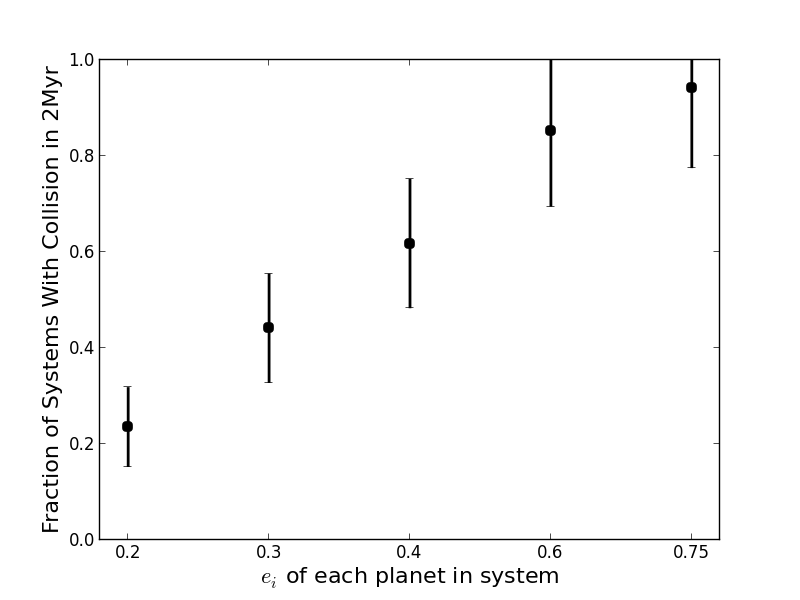
\includegraphics[trim=0cm 0cm 0.5cm 0.5cm, scale=0.48]{appendix/e_max_dyn.png}}
\caption{The fraction of \kep{} systems in our sample that go unstable within 2Myr if each planet is given an initial eccentricity of $e_i$. The error bars derived from Poisson statistics.}
\label{fig:emax_dyn}
\end{figure}

Each point in Figure~\ref{fig:emax_dyn} represents the fraction of systems in our sample having a collision within 2 Myr.
We can see that for $e_i = 0.3$, about half of the Kepler systems have had a collision. 
Thus from stability arguments, the maximum initial eccentricity that planets in our Kepler sample can have in order for $\sim 50\%$ of them to survive at least 2 Myr is $e_{max} \approx 0.3$.  

%%%%%%%%%%%%%%%%%%%%%%%%%%%%%%%%%%%%%%%%%%%%%%%%%%%
%%%%%%%%%%%%%%%%%%%%%%%%%%%%%%%%%%%%%%%%%%%%%%%%%%%
%%%%%%%%%%%%%%%%%%%%%%%%%%%%%%%%%%%%%%%%%%%%%%%%%%%
\onecolumn
\newpage
\section{Planet Sample}

\begin{center}
%\begin{longtable}{|c|c|c|c|p{2cm}|c|c|c|c|}
\begin{longtable}{rcrrrrrrr}
\caption[Portrait, single page table]{Kepler Systems Used In This Analysis} \\
 
\hline \hline \\[-0.1ex]
   \multicolumn{1}{c}{ {System}} &
   \multicolumn{1}{c}{ {Planet}} &
   \multicolumn{1}{c}{ {$P$ (days)}} &
   \multicolumn{1}{c}{ {near MMR}} &
   \multicolumn{1}{c}{ {$m_p/m_{\oplus}$}} &
   \multicolumn{1}{c}{ {$r_p/r_{\oplus}$}} &
   \multicolumn{1}{c}{ {$N_p$}}  &
   \multicolumn{1}{c}{ {$M/M_{\odot}$}} &
   \multicolumn{1}{c}{ {$R/R_{\odot}$}}  \\[0.5ex]\hline \hline \\[-2ex]
\endfirsthead

%\hline \kep{} System &  Planet Letter &  $P$ (days) & near MMR & $m_p/m_{\oplus}$ &  $r_p/r_{\oplus}$ & $N_p$ & $M/M_{\odot}$ &  $R/R_{\odot}$   \\\hline
KOI-142 & b & 10.95 & \checkmark & $8.7 \pm 2.5$ & $3.82 \pm 0.44$ & 2 & $0.96 \pm 0.04$ & $0.88 \pm 0.03$ \\  
 & c & 22.34 & \checkmark & $198.8 \pm 9.2$ & $6.82 \pm 1.09$ & & & \\  
\hline 
Kepler-120 & b & 6.31 & \checkmark & $  $ & $2.18 \pm 0.22$ & 2 & $  $ & $0.53 \pm 0.03$ \\  
 & c & 12.79 & \checkmark & $  $ & $1.53 \pm 0.11$ & & & \\  
\hline 
Kepler-127 & b & 14.44 & \checkmark & $  $ & $1.42 \pm 0.11$ & 3 & $  $ & $1.36 \pm 0.04$ \\  
 & c & 29.39 & \checkmark & $  $ & $2.62 \pm 0.11$ & & & \\  
 & d & 48.63 & & $  $ & $2.62 \pm 0.11$ & & & \\  
\hline 
Kepler-176 & b & 5.43 & & $  $ & $1.42 \pm 0.76$ & 3 & $  $ & $0.89 \pm 0.46$ \\  
 & c & 12.76 & \checkmark & $  $ & $2.62 \pm 1.31$ & & & \\  
 & d & 25.75 & \checkmark & $  $ & $2.51 \pm 1.31$ & & & \\  
\hline 
Kepler-183 & b & 5.69 & \checkmark & $  $ & $2.07 \pm 0.87$ & 2 & $  $ & $0.96 \pm 0.41$ \\  
 & c & 11.64 & \checkmark & $  $ & $2.29 \pm 0.98$ & & & \\  
\hline 
Kepler-221 & b & 2.8 & \checkmark & $  $ & $1.75 \pm 0.22$ & 4 & $0.72 \pm 0.05$ & $0.82 \pm 0.07$ \\  
 & c & 5.69 & \checkmark & $  $ & $2.95 \pm 0.33$ & & & \\  
 & d & 10.04 & & $  $ & $2.73 \pm 0.22$ & & & \\  
 & e & 18.37 & & $  $ & $2.62 \pm 0.22$ & & & \\  
\hline 
Kepler-244 & b & 4.31 & & $  $ & $2.73 \pm 1.2$ & 3 & $  $ & $0.8 \pm 0.34$ \\  
 & c & 9.77 & \checkmark & $  $ & $2.07 \pm 0.87$ & & & \\  
 & d & 20.05 & \checkmark & $  $ & $2.29 \pm 0.98$ & & & \\  
\hline 
Kepler-25 & b & 6.24 & \checkmark & $9.0 \pm 2.4$ & $2.62 \pm 0.0$ & 3 & $1.19 \pm 0.06$ & $1.31 \pm 0.02$ \\  
 & c & 12.72 & \checkmark & $14.3 \pm 2.7$ & $4.48 \pm 0.0$ & & & \\  
 & d & 123.0 && $89.9 \pm 13.7$ & $5.46 \pm 0.0$ & & & \\  
\hline 
Kepler-267 & b & 3.35 & \checkmark & $  $ & $1.97 \pm 0.11$ & 3 & $0.56 \pm 0.05$ & $0.56 \pm 0.02$ \\  
 & c & 6.88 & \checkmark & $  $ & $2.07 \pm 0.11$ & & & \\  
 & d & 28.46 & & $  $ & $2.29 \pm 0.11$ & & & \\  
\hline 
Kepler-27 & b & 15.33 & \checkmark & $41.8 \pm 5.0$ & $4.04 \pm 0.0$ & 2 & $0.65 \pm 0.16$ & $0.59 \pm 0.15$ \\  
 & c & 31.33 & \checkmark & $21.2 \pm 3.2$ & $4.91 \pm 0.0$ & & & \\  
\hline 
Kepler-272 & b & 2.97 & \checkmark & $  $ & $1.42 \pm 0.76$ & 3 & $0.79 \pm 0.05$ & $0.93 \pm 0.5$ \\  
 & c & 6.06 & \checkmark & $  $ & $1.75 \pm 0.98$ & & & \\  
 & d & 10.94 & & $  $ & $2.29 \pm 1.2$ & & & \\  
\hline 
Kepler-30 & b & 29.33 & \checkmark & $11.3 \pm 1.4$ & $3.93 \pm 0.22$ & 3 & $0.99 \pm 0.08$ & $0.95 \pm 0.12$ \\  
 & c & 60.32 & \checkmark & $640.0 \pm 50.0$ & $12.34 \pm 0.44$ & & & \\  
 & d & 143.34 & & $23.1 \pm 2.7$ & $8.84 \pm 0.55$ & & & \\  
\hline 
Kepler-305 & b & 5.49 & & $10.5 \pm 2.6$ & $3.6 \pm 0.87$ & 3 & $0.76 \pm 0.13$ & $0.79 \pm 0.05$ \\  
 & c & 8.29 & \checkmark & $6.0 \pm 2.4$ & $3.28 \pm 0.76$ & & & \\  
 & d & 16.74 & \checkmark & $  $ & $2.73 \pm 0.44$ & & & \\  
\hline 
Kepler-32 & f & 0.74 & & $  $ & $0.76 \pm 0.11$ & 5 & $0.54 \pm 0.02$ & $0.53 \pm 0.02$ \\  
 & e & 2.9 & \checkmark & $  $ & $1.53 \pm 0.11$ & & & \\  
 & b & 5.9 & \checkmark & $9.4 \pm 3.6$ & $2.18 \pm 0.22$ & & & \\  
 & c & 8.75 & & $7.7 \pm 5.0$ & $1.97 \pm 0.22$ & & & \\  
 & d & 22.78 & & $  $ & $2.73 \pm 0.11$ & & & \\  
\hline 
Kepler-326 & b & 2.25 & \checkmark & $  $ & $1.53 \pm 0.22$ & 3 & $0.98 \pm 0.05$ & $0.8 \pm 0.05$ \\  
 & c & 4.58 & \checkmark & $  $ & $1.42 \pm 0.11$ & & & \\  
 & d & 6.77 & & $  $ & $1.2 \pm 0.11$ & & & \\  
\hline 
Kepler-327 & b & 2.55 & \checkmark & $  $ & $1.09 \pm 0.11$ & 3 & $0.55 \pm 0.05$ & $0.49 \pm 0.02$ \\  
 & c & 5.21 & \checkmark & $  $ & $0.98 \pm 0.11$ & & & \\  
 & d & 13.97 & & $  $ & $1.75 \pm 0.11$ & & & \\  
\hline 
Kepler-328 & b & 34.92 & \checkmark & $28.5 \pm 12.9$ & $2.29 \pm 0.98$ & 2 & $1.15 \pm 0.22$ & $1.06 \pm 0.44$ \\  
 & c & 71.31 & \checkmark & $39.4 \pm 13.6$ & $5.46 \pm 2.29$ & & & \\  
\hline 
Kepler-384 & b & 22.6 & \checkmark & $  $ & $1.09 \pm 0.33$ & 2 & $0.76 \pm 0.05$ & $0.88 \pm 0.25$ \\  
 & c & 45.35 & \checkmark & $  $ & $1.09 \pm 0.33$ & & & \\  
\hline 
Kepler-386 & b & 12.31 & \checkmark & $  $ & $1.42 \pm 0.76$ & 2 & $0.74 \pm 0.05$ & $0.77 \pm 0.43$ \\  
 & c & 25.19 & \checkmark & $  $ & $1.64 \pm 0.87$ & & & \\  
\hline 
Kepler-396 & b & 42.99 & \checkmark & $75.5 \pm 11.8$ & $3.49 \pm 1.31$ & 2 & $0.85 \pm 0.13$ & $1.06 \pm 0.39$ \\  
 & c & 88.5 & \checkmark & $17.9 \pm 2.8$ & $5.35 \pm 1.97$ & & & \\  
\hline 
Kepler-48 & b & 4.78 & \checkmark & $14.3 \pm 4.3$ & $2.18 \pm 0.0$ & 3 & $0.88 \pm 0.06$ & $0.89 \pm 0.05$ \\  
 & c & 9.67 & \checkmark & $9.8 \pm 3.3$ & $3.17 \pm 0.0$ & & & \\  
 & d & 42.9 & & $7.93 \pm 4.6$ & $2.07 \pm 0.11$ & & & \\  
\hline 
Kepler-56 & b & 10.5 & \checkmark & $22.1 \pm 3.9$ & $6.55 \pm 0.33$ & 2 & $1.32 \pm 0.13$ & $4.23 \pm 0.15$ \\  
 & c & 21.4 & \checkmark & $181.0 \pm 21.0$ & $9.83 \pm 0.44$ & & & \\  
\hline 
Kepler-57 & b & 5.73 & \checkmark & $118.1 \pm 24.1$ & $2.18 \pm 0.0$ & 2 & $0.83 \pm 0.05$ & $0.73 \pm 0.0$ \\  
 & c & 11.61 & \checkmark & $7.4 \pm 9.4$ & $1.53 \pm 0.0$ & & & \\  
\hline 
Kepler-79 & b & 13.48 & \checkmark & $  $ & $2.62 \pm 0.76$ & 4 & $1.1 \pm 1.63$ & $1.4 \pm 0.25$ \\  
 & c & 27.4 & \checkmark & $  $ & $2.73 \pm 0.87$ & & & \\  
 & d & 52.09 & & $  $ & $7.64 \pm 1.42$ & & & \\  
 & e & 81.07 & & $  $ & $3.38 \pm 0.66$ & & & \\  
\hline 
Kepler-81 & b & 5.96 & \checkmark & $  $ & $2.4 \pm 0.44$ & 3 & $0.64 \pm 0.38$ & $0.59 \pm 0.03$ \\  
 & c & 12.04 & \checkmark & $  $ & $2.4 \pm 0.33$ & & & \\  
 & d & 20.84 & & $  $ & $1.2 \pm 0.33$ & & & \\  
\hline 
Kepler-83 & d & 5.17 & & $  $ & $1.97 \pm 0.11$ & 3 & $0.66 \pm 0.41$ & $0.59 \pm 0.03$ \\  
 & b & 9.77 & \checkmark & $  $ & $2.84 \pm 0.44$ & & & \\  
 & c & 20.09 & \checkmark & $  $ & $2.4 \pm 0.33$ & & & \\  
\hline 
Kepler-9 & d & 1.59 & & $  $ & $1.64 \pm 0.22$ & 3 & $1.07 \pm 0.05$ & $1.02 \pm 0.05$ \\  
 & b & 19.24 & \checkmark & $80.09 \pm 4.13$ & $9.5 \pm 0.76$ & & & \\  
 & c & 38.91 & \checkmark & $54.35 \pm 4.13$ & $9.28 \pm 0.76$ & & & \\ 
\hline 

\label{tab:kepsys}
\end{longtable}
\end{center}
\twocolumn

\end{document}


\end{document}

%%%%%%%%%%%%%%%%%%%%%%%%%%%%%%%%%%%%%%%%%%%%%%%%%%%%%%%%%%%%%%%%%%%%%%
%%  End of UT-THESIS.TEX
%%%%%%%%%%%%%%%%%%%%%%%%%%%%%%%%%%%%%%%%%%%%%%%%%%%%%%%%%%%%%%%%%%%%%%
